\documentclass[a4paper,12pt]{article}

% PACKAGES
\usepackage[T1]{fontenc}
\usepackage[utf8]{inputenc}
\usepackage[french]{babel}
\usepackage{csquotes}
\usepackage[notes,backend=biber]{biblatex-chicago}
\bibliography{biblio/mabiblio.bib}
\usepackage{amsmath}
\usepackage{amssymb}
\usepackage{amsthm}
\usepackage{amscd}
\usepackage{lmodern} % OBLIGATOIRE
\usepackage{textcomp}
\usepackage{graphicx}
\usepackage{hyperref}
\usepackage{sectsty}

% MISE EN PAGE
\setlength{\voffset}{-3.75cm}
\setlength{\hoffset}{-2.6cm}
\setlength{\oddsidemargin}{2.5cm} % OBLIGATOIRE
\setlength{\evensidemargin}{2.5cm} % OBLIGATOIRE
\setlength{\topmargin}{3.1cm} % OBLIGATOIRE
\setlength{\headheight}{0in}
\setlength{\headsep}{0in}
\setlength{\topskip}{0in}
\setlength{\parindent}{0pt}
\setlength{\parskip}{1ex plus0.4ex minus0.2ex}
\setlength{\textwidth}{16cm} % OBLIGATOIRE
\setlength{\textheight}{24.7cm} % OBLIGATOIRE
\renewcommand{\baselinestretch}{1.5} % OBLIGATOIRE
\flushbottom
\setcounter{page}{1}
\setcounter{tocdepth}{3}
\usepackage{helvet} % OBLIGATOIRE
\renewcommand{\familydefault}{\sfdefault} % OBLIGATOIRE

% PERSO
\newcommand{\guill}[1]{«~#1~»}
\newcommand{\guilldeux}[1]{“#1”}
\newcommand{\eme}[0]{$^\text{e}$}
\newcommand{\Ier}[0]{I$^\text{er}$} \newcommand{\IIe}[0]{II\eme} \newcommand{\IIIe}[0]{III\eme} \newcommand{\IVe}[0]{IV\eme} \newcommand{\Ve}[0]{V\eme} \newcommand{\VIe}[0]{VI\eme} \newcommand{\VIIe}[0]{VII\eme} \newcommand{\VIIIe}[0]{VIII\eme} \newcommand{\IXe}[0]{IX\eme} \newcommand{\Xe}[0]{X\eme} \newcommand{\XIe}[0]{XI\eme} \newcommand{\XIIe}[0]{XII\eme} \newcommand{\XIIIe}[0]{XIII\eme} \newcommand{\XIVe}[0]{XIV\eme} \newcommand{\XVe}[0]{XV\eme} \newcommand{\XVIe}[0]{XVI\eme} \newcommand{\XVIIe}[0]{XVII\eme} \newcommand{\XVIIIe}[0]{XVIII\eme} \newcommand{\XIXe}[0]{XIX\eme} \newcommand{\XXe}[0]{XX\eme} \newcommand{\XXIe}[0]{XXI\eme}
\newcommand{\bigO}[1]{\mathcal O\left( #1 \right)}
\newcommand{\bigOmega}[1]{\Omega\left( #1 \right)}
\newcommand{\bigTheta}[1]{\Theta\left( #1 \right)}
\newcommand{\zitat}[2]{\#Citation(#2)\#}
\newcommand{\maze}[0]{\emph{m\symbol{64}ze\textdegree2}}
\newcommand{\tpp}[0]{[\dots]}
\newcommand{\module}[1]{\texttt{\textsc{#1}}}
\newcommand{\patch}[1]{[\texttt{#1}]}
\newcommand{\cicite}[1]{{\footnotesize[#1]}}








\title{\Large Internship report \\ \LARGE Computational analysis of jazz chord sequences}
\author{\normalsize Romain \textsc{Versaevel}, M1 Informatique Fondamentale, ENS de Lyon\\
\normalsize Tutored by David \textsc{Meredith}, Associate Professor, Aalborg University,\\
\normalsize leader of the Music Informatics and Cognition group\\}
\date{\today}

\begin{document}

%\maketitle
%\newpage

\tableofcontents

\newpage

\section{Introduction}

Dans la deuxième moitié du \XXe~siècle, l'informatique moderne, qui était née dans les sphères militaire et académique, a progressivement conquis et révolutionné de nombreux autres domaines d'application. À la fois science centrée sur le calcul et la logique, et technologie dont les principaux représentants sont l'ordinateur et le réseau, elle est aujourd'hui entrée dans les mœurs, conduisant à l'apparition d'une \guill{culture numérique} mondiale. Si bien que, comme le souligne l'historien Philippe Breton, \guill{la question qui est aujourd’hui d'actualité en matières d'informatique est celle de la maîtrise des enjeux que soulève son insertion dans la vie quotidienne}\footnote{Pour un exemple d'étude approfondie et récente du rôle joué par l'informatique dans divers secteurs, voir \cicite{Cortada,~2004}.} \cicite{Breton,~1987,~avant-propos}. Le champ artistique, qui a toujours exploité les ressources de la technologie, ne fait pas exception dans le processus d'assimilation de l'informatique. L'ordinateur a bouleversé les formes et les disciplines --- réalité augmentée, dispositifs multimédias, œuvres interactives\dots~---, conduisant au développement de l'\emph{art numérique}.

L'objet de ce document est d'étudier cet investissement de l'art contemporain par l'informatique, à travers le cas du compositeur contemporain autrichien Karlheinz Essl. Dans son œuvre, Essl a en effet assimilé les technologies numériques et se les est appropriées en leur donnant une place de premier plan, ce qui fait de lui un exemple particulièrement intéressant d'interface entre art et technique informatique. Il s'est ainsi spécialisé dans la musique algorithmique, c'est-à-dire le recours à des méthodes formelles, généralement appliquées par un programme informatique, pour la composition. Puis, grâce aux progrès technologiques entraînant la diminution des temps de calcul, Essl a conjugué ces méthodes de composition informatiquement automatisée avec des dispositif de production de son en temps réel, élaborant ainsi la notion de \guill{\emph{composition en temps réel}}.

Notre démarche sera de faire l'étude historique de ce compositeur et de sa pratique. Le code des programmes écrits par Essl est la principale source sur laquelle reposent nos analyses. À travers ces programmes, nous montrerons que les innovations conceptuelles réalisées par Essl, qui représentent de véritables apports qualitatifs sur le plan artistique, l'ont été dès le moment où le progrès technologique incrémental les a rendues possibles.

Essl a fait l'objet de plusieurs travaux biographiques\footnote{En particulier \cicite{Ehrler,~1999}, \cicite{Felber,~2007}, \cicite{Essl~et~Kühnelt,~2006/2007}, \cicite{Dobretsberger,~2006}, \cicite{Sinkovicz,~2005}, \cicite{Klein,~2013}.}, et ses œuvres sont régulièrement décrites, commentées et analysées\footnote{Par exemple dans \cicite{Collins,~2010,~chap.~8} ou \cicite{Rowe,~2004,~p.~306-308}.}. Cependant aucun de ces travaux n'a l'ampleur de celui-ci. En outre, ils se concentrent sur les aspects artistique et esthétique. L'originalité du présent document est d'approcher Essl comme un acteur historique de la révolution numérique, et sa production comme source au-delà de sa qualité artistique.

%\zitat{Le dessinateur, le peintre, le musicien, le cinéaste ou le vidéaste, l'architecte, le designer, ne travaillent plus avec des crayons, des gommes, des règles, des pigments, des pinceaux, du marbre ou du fer, des éclairages et des caméras, le laser ou le téléphone, mais avec des symboles : ceux qui constituent le langage des programmes informatiques. Les matériaux et les outils numériques sont essentiellement d'ordre symbolique et langagier.}
%{L'art numérique, p. 25}
%ANNONCER LES CONCLUSIONS ?

%\zitat{Toutes ces relations entre l'art et la science au cours de \XIXe~et \XXe~siècles s'établissent sur un mode \guill{métaphorique}. La science fournit à l'art des représentations ou des modèles abstraits du monde que celui-ci transfigure en images sensibles ; l'art opère par substitution analogique, transfert et déplacement de sens. La science donne des idées, propose des conceptions du monde, de la réalité, inspire, suggère, travaille l'art par-dessous. Les artistes y trouvent souvent la confirmation de certaines intuitions ou une stimulation pour l'imagination. Elle se différencie en cela de la technique. Car les techniques sont, outre des processus pour transformer et produire le monde, des manières de le percevoir. La technique n'agit pas en proposant des idées, des visions abstraites, elle agit sur la perception. Directement quand elle procure aux artistes des moyens de figuration, telle la photographie, dont les répercussions sur la peinture furent très importantes, mais aussi indirectement, en modifiant l'\emph{habitus} perceptif des sociétés dans lequel s'enracine une bonne partie des pratiques artistiques et culturelles.}
%{L'art numérique, p. 33}

Une première partie décrit le parcours du compositeur, en montrant le parallèle avec l'expansion du rôle de l'informatique dans la société, et la construction des notions importantes de son œuvre. La seconde partie, grâce à l'étude en détail des programmes d'Essl ---~sa bibliothèque \emph{Realtime Composition Library} (1993-) et sa pièce la plus renommée, la \emph{Lexikon-Sonate} (1992-2007) --- interroge ces notions, et montre en quoi l'ordinateur est un outil dans son processus créatif.

\section{Parcours de Karlheinz Essl}

Nous distinguons quatre parties dans le parcours de Karlheinz Essl, dont un portrait est visible sur la figure \ref{portrait}. D'abord ses premiers pas de musiciens et ses études, qui voient la formation des influences qui marqueront tout son œuvre. Ensuite, l'assimilation de la \emph{musique algorithmique} qui coïncide avec ses premières utilisations de l'ordinateur, puis le bouleversement de cette démarche provoqué par la rencontre avec le \emph{temps réel}. Enfin, le mouvement du compositeur vers le performeur, marqué par le recours à l'improvisation et aux pratiques artistiques collaboratives.

\begin{figure}[!h]
\begin{center}
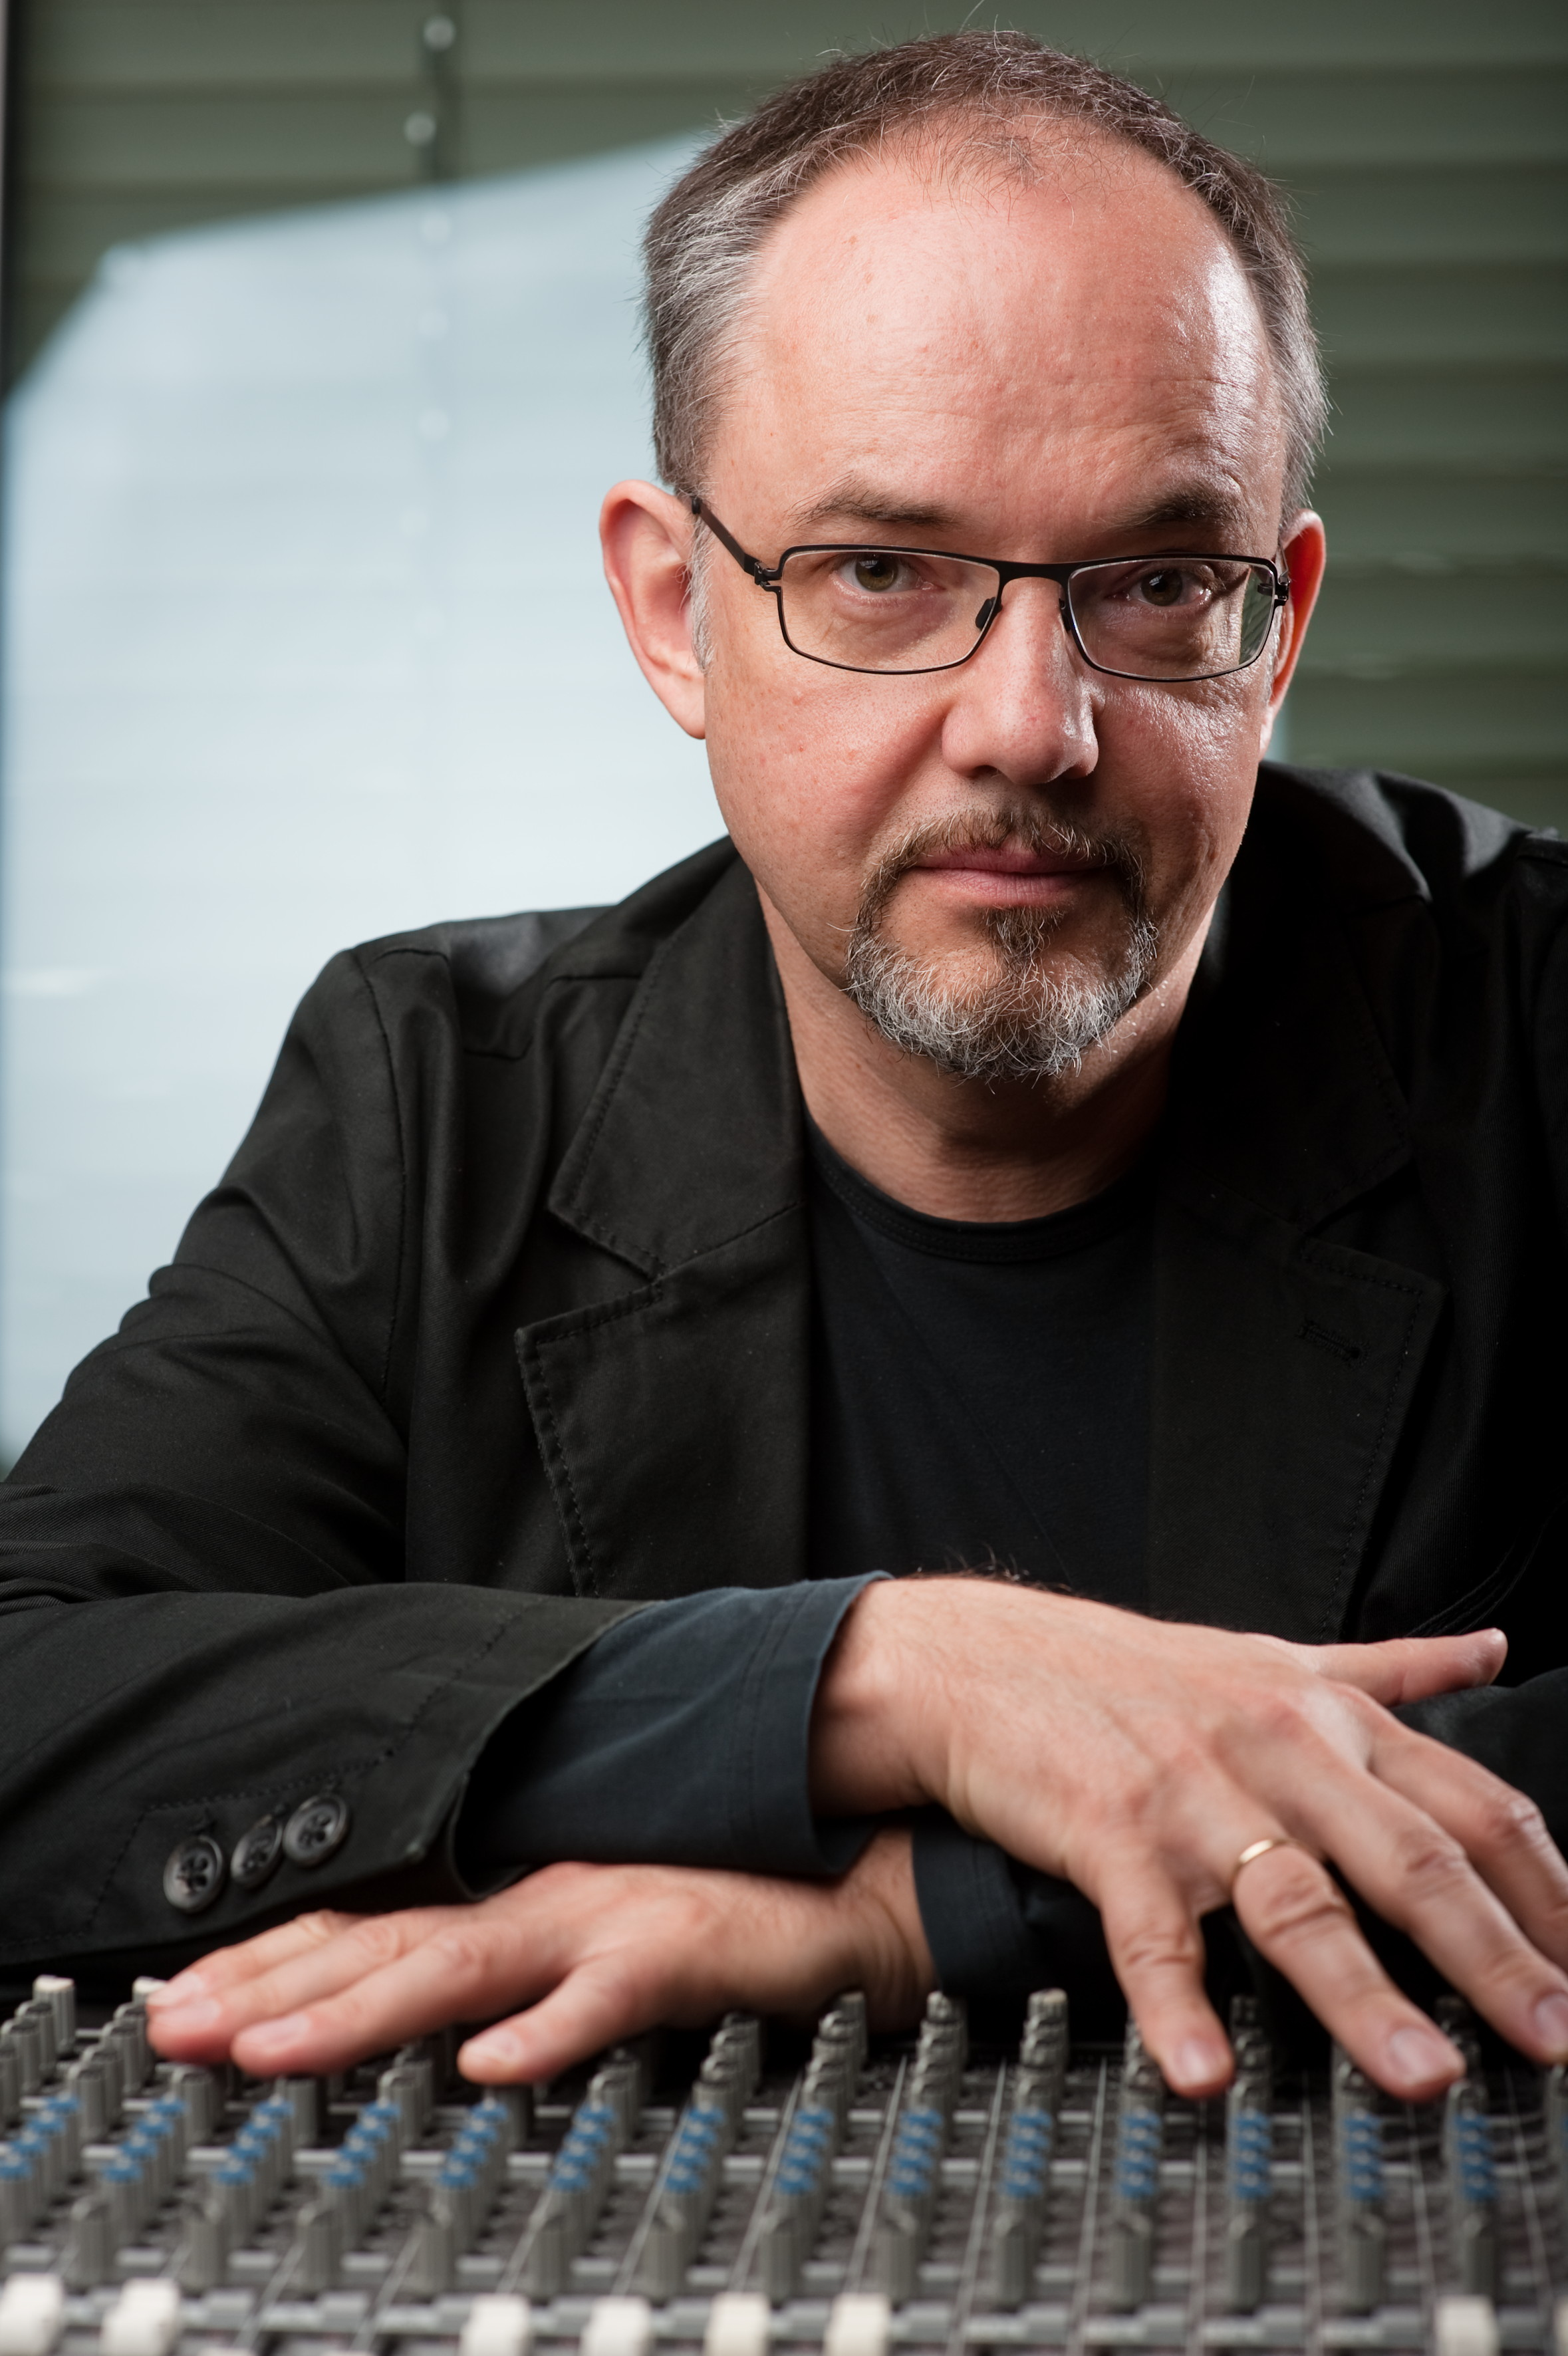
\includegraphics[width=5cm]{images/essl.jpg}
\caption{\footnotesize Portrait de Karlheinz Essl en 2009. Photo \copyright~Johannes Tichy}
\label{portrait}
\end{center}
\end{figure}

\subsection{Formation : entre rock et éducation classique}

Né le 15 août 1960 à Vienne, Karlheinz Essl est issu d'un milieu aisé et cultivé. Son père, Karlheinz Essl senior, est un entrepreneur, qui a fait fortune en fondant la chaîne de magasins de bricolages bauMax\footnote{Entreprise dissoute en 2015, suite aux conséquences de la crise financière de 2007.}. Il est aussi connu comme collectionneur d'art, ayant acquis avec sa femme Agnes de nombreuses œuvres contemporaines à partir des années 1970, collection qui l'a conduit à faire construire son propre musée, le \emph{Essl Museum}, dans la ville de Klosterneuburg située sur le Danube à quelques kilomètres au nord de Vienne.

Karlheinz junior est ainsi au contact d'un environnement culturel savant\footnote{On parle de \guill{musique savante} pour désigner la tradition musicale occidentale fortement structurée et théorisée, qui est généralement opposée aux musiques traditionnelle et populaire. Dans la suite de ce document on préférera ce terme à celui de \guill{musique classique}, fréquemment employé mais prêtant à confusion (cette musique \guill{classique} n'étant pas limitée à la période classique (1750-1820)).} dès son plus jeune âge. Il étudie le piano à partir de l'âge de sept ans. Il explique cependant que cette expérience lui a déplu et qu'il n'a vraiment apprécié la musique que lorsque, adolescent, il s'est intéressé à la musique rock \cicite{Ehrler,~1999}. Il prend alors part à plusieurs groupes et s'initie, en autodidacte, à la guitare électrique puis à la contrebasse. Néanmoins, ce n'est pas le rock \guill{grand public} qui attire Essl, qui cite plus volontiers des groupes avant-gardistes ou expérimentaux comme \emph{Gentle Giant} ou \emph{Can}. C'est à travers ce dernier qu'Essl découvre la musique du compositeur allemand Karlheinz Stockhausen (1928-2007) (deux membres de \emph{Can}, le bassiste Holger Czukay et le claviériste Irmin Schmidt ont tous deux été ses élèves). Âgé de 15 ans, il achète un vinyle de Stockhausen, décrivant la découverte comme un véritable \guill{choc}\footnote{\guill{À la maison, j'ai mis mon casque et écouté le vinyle. J'étais complètement sous le choc. À l'époque, je trouvais cette musique atroce, qui pourtant m'a emballé.} \cicite{Essl~et~Hötzenecker,~2016}.}. Cet engouement naissant pour la musique électronique le conduira même à construire un petit synthétiseur \cicite{Essl~et~Kühnelt,~2006/2007}.

Lorsqu'il arrive dans les études supérieures, Essl, bien qu'ayant suivi une formation en chimie\footnote{\emph{Oberstufe Gymnasium}, parcours du système scolaire allemand et autrichien équivalent au lycée (\emph{Gymnasium}), mais plus long d'un an, ce qui permet d'approfondir une discipline de spécialité.} décide de se consacrer à la musique. Cette décision est prise à l'encontre de ses parents, qui le destinaient à prendre la succession de la direction de l'entreprise familiale (ce que fera finalement son frère cadet, Martin Essl). Reçu à la prestigieuse Académie de musique et des arts du spectacle de Vienne (\emph{Universität für Musik und darstellende Kunst Wien}), il y étudie l'harmonie et le contrepoint avec Alfred Uhl (1909-1992), la contrebasse avec Heinrich Schneikart (1929-2008), et la composition auprès de Friedrich Cerha (1926-). Progressivement il va abandonner la contrebasse pour se consacrer exclusivement à l'analyse musicale et à la composition, suivant en outre des cours de Dieter Kaufmann sur la musique électro-acoustique. 	Ce parcours académique le conduit à rédiger une thèse sur la \guill{pensée-synthèse} chez Anton Webern sous la direction du musicologue Hans Schneider, achevée en 1991 \cicite{Essl,~1991}. L'influence de la musique de Webern, et plus généralement de la musique sérielle (voir ci-après), traverse l'ensemble de l'œuvre d'Essl. Il a notamment rendu hommage à Webern à l'occasion du soixantième anniversaire de sa mort, à travers un morceau et un programme (\emph{WebernSpielWerk} et \emph{WebernUhrWerk}, 2005).

Au cours de ses études, Essl fait deux rencontres décisives. D'abord, en 1985, il rend visite à son ami Gerhard Eckel en stage à l'Institut de Sonologie (\emph{Instituut voor Sonologie}) de La Haye (Pays-Bas), l'un des premiers centres de recherche en musique électronique et musique informatique. C'est à cette occasion qu'il fait la connaissance, en partie par hasard, de Gottfried Michael Koenig (1926-), compositeur allemand pionnier de la musique algorithmique, qui dirige l'Institut depuis 1964. Essl trouve la partition d'un quatuor écrit par Koenig (\emph{Streichquartett 1959}, 1959) et, ayant des difficultés à l'analyser, contacte celui-ci, qui lui apprend qu'il a utilisé des opérations de hasard dans sa composition. Les deux compositeurs correspondent et collaborent depuis, Essl ayant même été invité à contribuer à l'élaboration de \emph{Projekt 3}, projet resté inachevé faisant suite aux \emph{Projekt 1} (1964) et \emph{Projekt 2} (1966), premiers programmes pour la Composition Assistée par Ordinateur (CAO). Puis, en 1988, Essl rencontre John Cage (1912-1992), compositeur américain emblématique du \XXe~siècle. Il connaît déjà son œuvre mais peut l'approcher en personne lors d'un concert donné en son honneur à Vienne . L'œuvre de Cage marque profondément celle d'Essl, qui lui rend d'ailleurs hommage dans deux de ses créations : \emph{In The Cage} (1987) et \emph{FontanaMixer} (2004).

Cette période de formation, qui s'achève avec jusqu'à la soutenance de thèse en 1991, voit se former le style d'Essl. On peut y identifier ses principales influences théoriques. \\
D'abord, il y a le \textbf{sérialisme}, auquel l'a initié son professeur Friedrich Cerha\footnote{Dans \cicite{Essl~et~Pagano,~2009}, Essl précise qu'avant de commencer sa formation auprès de Cerha ses goûts le portaient plutôt vers des mouvances opposées comme le néo-classicisme.}. Ce mouvement, fondé à Vienne au début du \XXe~siècle par la seconde école de Vienne (Arnold Schönberg, Alban Berg et Anton Webern), élabore à l'origine des techniques d'inspiration arithmétique pour éradiquer systématiquement la tonalité, le langage musical utilisé dans toute la musique savante occidentale depuis le \XVIIIe~siècle, qui limite le matériau employé dans chaque composition (par exemple, la tonalité de do majeur n'utilise que les touches blanches du piano). L'objet central du sérialisme est la \emph{série}, qui est un ordonnancement exhaustif du matériau disponible. La série dodécaphonique fait ainsi se succéder les douze hauteurs de la gamme chromatique sans en répéter aucun, évitant ainsi toute ressemblance avec une tonalité identifiable ; des séries peuvent aussi être utilisées pour contrôler les volumes, les rythmes, etc.\footnote{La présente étude ne nécessite pas une connaissance pointue du sérialisme sur le plan esthétique. Il faut essentiellement en retenir la volonté de contrôler la musique par des procédés mathématiques. Le lecteur qui souhaiterait en savoir plus est invité à consulter par exemple \cicite{Wodon,~2014}.} De très nombreux compositeurs du \XXe~siècle se réclament du sérialisme et l'ont développé, parmi lesquels Stockhausen et Koenig, mais aussi Pierre Boulez (1925-2016), Luigi Nono (1924-1990), Luciano Berio (1925-2003)\dots~Sur le plan esthétique, l'école sérielle va de pair avec la philosophie d'Adorno, lui-même compositeur, qui promeut la \textbf{Nouvelle Musique} (\emph{Neue Musik}), marquée par l'injonction avant-gardiste. Cette théorie esthétique, présente dans toutes les disciplines de l'art contemporain, exige des artistes une innovation radicale permanente pour mériter ce statut\footnote{\guill{Le paradigme adornien d'une négativité en acte dans l'œuvre d'art se lit comme une injonction pour l'art moderne, et en partie pour l'art contemporain, d'avoir à intégrer l'action impérative de l'avant-garde. L'art se doit d'être critique --- traduisons : avant-gardiste --- et cet impératif s'ajoute à ceux déjà institués par les fondations précédentes.} \cicite{Cauquelin,~2010, p. 59}. Pour plus de détails sur la philosophie esthétique d'Adorno, voir \cicite{Adorno,~1949} et \cicite{Adorno,~1970}.}. Elle se manifeste dans l'intérêt qu'Essl portera à l'ordinateur et sa participation à l'avant-garde. \\
Les autres influences notables sont celles des trois compositeurs déjà cités : \textbf{Stockhausen}, \textbf{Koenig} et \textbf{Cage}. Tous trois ont été parmi les premiers musiciens à explorer les possibilités de l'\emph{œuvre ouverte}\footnote{Telle que définie par Umberto Eco dans \emph{L'Œuvre ouverte} \cicite{Eco,~1962}. Cette notion est décrite plus en détail dans la section \ref{lsanalyse}.} et du hasard, problématiques très présentes dans l'œuvre d'Essl. Koenig a même affirmé même que \guill{la maîtrise du hasard par le compositeur est un problème centrale de la musique actuelle} \cicite{Koenig,~1962,~p.~813}. Le hasard joue plus généralement un rôle essentiel dans l'art du \XXe~siècle, qui cherche notamment à s'approprier les notions issues de la théorie du chaos et de la physique quantique. De Stockhausen, on retrouve l'intérêt porté au son et en particulier au son de synthèse, avec l'intégration de la musique électronique dans la musique savante. De Koenig, une paternité technique directe, puisqu'il a initié Essl à la musique algorithmique. De Cage, la recherche de formes radicalement nouvelles, en particulier l'événement, la performance. Le compositeur Andrew Gerzso résume ainsi le terreau dans lequel Essl a pu développer son œuvre : \guill{Schönberg a porté un coup terrible à la tonalité et Cage à ce qui fait l'essence d'une œuvre --- ouvrant la voie à la notion de \emph{work-in-progress} ou encore d'\emph{œuvre ouverte}} \cicite{Assayag~et~al.,~2009,~p.~1}. \\
Enfin, la dernière influence notable d'Essl est d'ordre philosophique ; il s'agit du \emph{constructivisme radical}, auquel le compositeur a même dédié un essai en 1992 \cicite{Essl,~1992}. Cette épistémologie repose sur l'idée que la \guill{connaissance} est une construction de l'esprit par rapport au monde, qui peut de fait varier d'un individu à l'autre, sans qu'il soit possible de parler de \guill{vérité}. Essl résume ainsi l'application de ce courant de pensée à sa pratique artistique : \guill{La musique ne se produit donc pas seulement dans la salle de concert, mais principalement dans la tête de l'auditeur. Savoir que le monde est construit par les perceptions individuelles plutôt que la simple illustration d'une réalité extérieure est lourd de conséquences pour la composition musicale. Cela fait en effet de l'auditeur un co-créateur.} \cicite{Essl,~2008}

Bien que le rock ait joué un rôle décisif, à la fois en étant la source de la passion qui a décidé Essl à faire des études de musique, et en l'amenant à Stockhausen et à la musique électronique, la formation du compositeur est avant tout classique, académique, savante. Elle est l'occasion pour lui de forger ses premières influences importantes, qui le suivront toute sa carrière, et de manifester une inclination favorable pour la musique algorithmique.

\subsection{Vers la musique algorithmique}
\label{parcoursalgo}

On l'a vu, la rencontre avec Gottfried Michael Koenig a amené Essl à s'intéresser à la musique algorithmique. Cet intérêt d'abord théorique connaît par la suite de nombreux développements sur le plan pratique, qui se construisent parallèlement à la relation entre Essl et l'ordinateur.

Ici, il convient de préciser ce que signifie ce terme de \guill{musique algorithmique}, et, pour commencer, ce qu'est un algorithme. Le mot \guill{algorithme}, forgé à partir du nom du mathématicien perse du \IXe~siècle Muhammad al-Khuw\=arizm\=\i, est défini\footnote{Pour une caractérisation plus poussée, qui n'est pas nécessaire ici, se reporter à \cicite{Knuth,~1998}.} par le comme un \guill{ensemble de règles opératoires dont l'application permet de résoudre un problème énoncé au moyen d'un nombre fini d'opérations} \cicite{Larousse~2016}. Dans ce sens, une recette de cuisine aussi bien que la méthode pour poser une multiplication sont des algorithmes. La composition algorithmique est alors simplement \guill{la création d'algorithmes dont le produit a des conséquences musicales notables et utiles au compositeur, allant de la production et de l'exploration de matériaux musicaux à la génération d'œuvres complètes} \cicite{Collins,~2010,~p.~299}. \\
Au sens large, la musique algorithmique possède donc une histoire séculaire\footnote{Cette remarque n'est pas seulement anecdotique : elle montre que l'histoire de la musique est imprégnée d'une culture algorithmique, qui explique que l'informatique ait trouvé un écho important dans cette discipline}. Tous les traités mettant en place des systèmes de règles pour l'organisation d'une composition en participent, dont le plus ancien connu, intitulé \emph{Musica enchiriadis} (d'auteur inconnu), remonte au \IXe~siècle. Le contrepoint rigoureux illustré par exemple dans \emph{L'art de la fugue BWV 1080} (1750) de Johann Sebastian Bach a une essence algorithmique, de même que, de manière totalement explicite, les jeux musicaux comme le \emph{müsikalisches Würfelspiel K.294d} (jeu de dé musical, 1792) de Mozart ou le jeu de \guill{cartes musiciennes} de la figure \ref{cartesajouer}. \\
Mais l'essor de la notion d'algorithme se fait conjointement avec l'avènement de l'informatique. Les ordinateurs sont en effet des machines capables d'appliquer des algorithmes de traitement de données et d'information ; ce sont en outre des machines \emph{programmables}, autrement dit non-spécialisées, auxquelles leur utilisateur peut confier \emph{n'importe quelle} tâche algorithmique, pourvu qu'il la formule dans un langage de programmation. Dans le domaine artistique, l'informatique musicale (\emph{computer music}) a exploré très tôt les possibilités offertes par les algorithmes, à la fois pour la composition et l'analyse musicologique de morceaux existants. Dans les années 1960 et 1970, ces deux axes contribuent à la formation de l'informatique musicale (\emph{computer music}) comme une discipline à part entière, avec l'ouverture de nombreux instituts dédiés à travers le monde et d'organes de communication scientifique : \emph{International Computer Music Conference} à partir de 1974, \emph{Computer Music Journal} à partir de 1977. Le traitement informatique du signal sonore (transformation et synthèse) n'est arrivé que plus tard\footnote{On peut tout de même citer les premières expériences pour faire jouer de la musique par ordinateur, sur le CSIRAC de l'université de Melbourne et le Ferranti Mark I de l'université de Manchester, toutes deux en 1951. Dans les deux cas, un synthétiseur simple jouait des mélodies populaires (\emph{God Save The King}, \emph{Baa Baa Black Sheep}, \emph{Colonel Boggey March}\dots) fournies à l'ordinateur.}. Cela s'explique par le fait que les données audio sont beaucoup plus volumineuses que les données symboliques nécessaires à la composition (des nombres pour représenter les hauteurs, durées\dots~des notes), et nécessitent des interfaces de conversion complexes (carte son). La musique électronique possède en outre une avance considérable dans ce domaine, qu'elle explore depuis le début du siècle ---~le premier instrument électronique de synthèse musicale, le Telharmonium, est construit en 1906. Dans les années 1980, quand Essl entre véritablement en contact avec les ordinateurs, l'informatique commence à rattraper ce retard ; elle permet de réaliser des synthèses et transformations inédites, impossibles avec la seule électronique, mais les calculs nécessitent encore un temps important. \\
La première partition générée par un ordinateur est l'\emph{Illiac Suite}\footnote{Voir \cicite{Hiller~et~Isaacson,~1979}.}, qui paraît en 1957. Elle est réalisée grâce à un programme conçu par Lejaren Hiller et Leonard Issacson, sur le superordinateur ILLIAC I, construit à l'université de l'Illinois en 1952. Les travaux se multiplient rapidement par la suite, tant en musique que dans les autres arts, si bien que l'on parle de \guill{révolution algorithmique}. Toujours en 1957, Iannis Xenakis (1922-2001) a recours à un ordinateur qui l'assiste dans des calculs pour un enregistrement de sa pièce \emph{Diamorphoses} ; et en 1964, c'est \emph{Projekt 1} de Koenig qui voit le jour. L'ordinateur permet d'assouvir deux quêtes de l'art de la deuxième moitié du \XXe~siècle, le recours au hasard qui désacralise la figure de l'auteur, et les recherches formelles, qui s'expriment dans les algorithmes\footnote{En littérature, ces deux tendances sont par exemple illustrées respectivement par le mouvement surréaliste et par l'OuLiPo.}. Dans une synthèse sur le sujet rédigée en 2007 \cicite{Essl,~2007}, Essl décrit plusieurs chemins d'appropriation de l'ordinateur par les initiateurs de la musique algorithmique : musique générative (dont sa propre démarche s'inspire, voir ci-dessous), automatisation de procédés d'écriture comme ceux du sérialisme, et investigation du hasard (comme les \guill{principes aléatoires} de Koenig ou la \guill{musique stochastique} de Xenakis).

\begin{figure}[!h]
\begin{center}
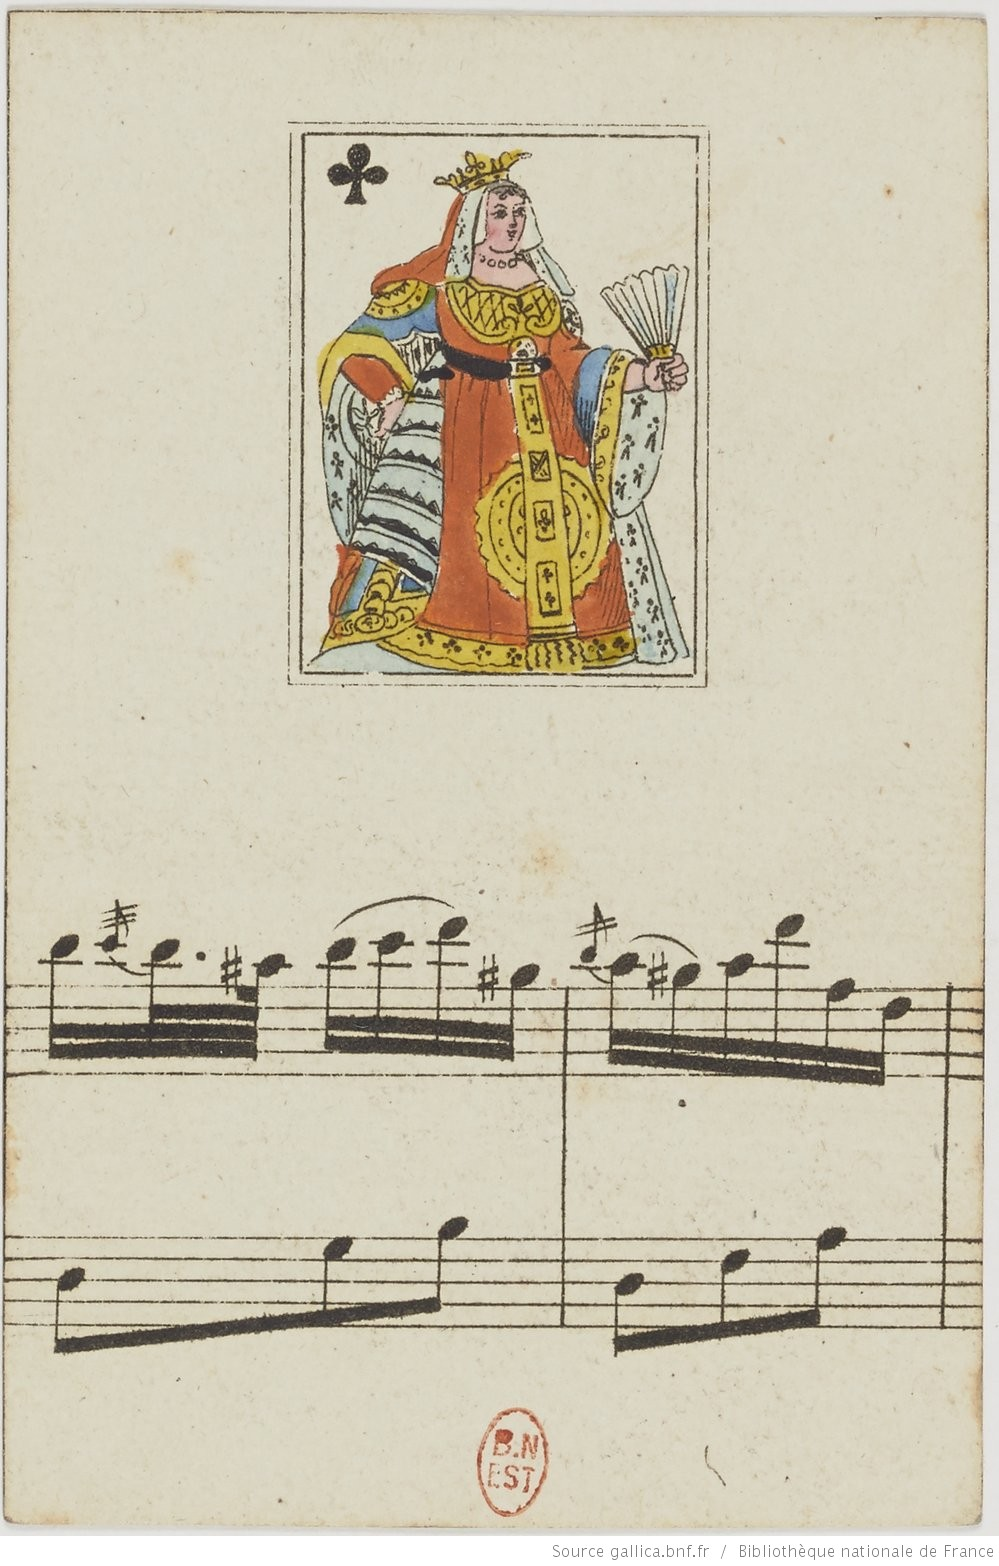
\includegraphics[height=5cm]{images/carte1.jpg}~~
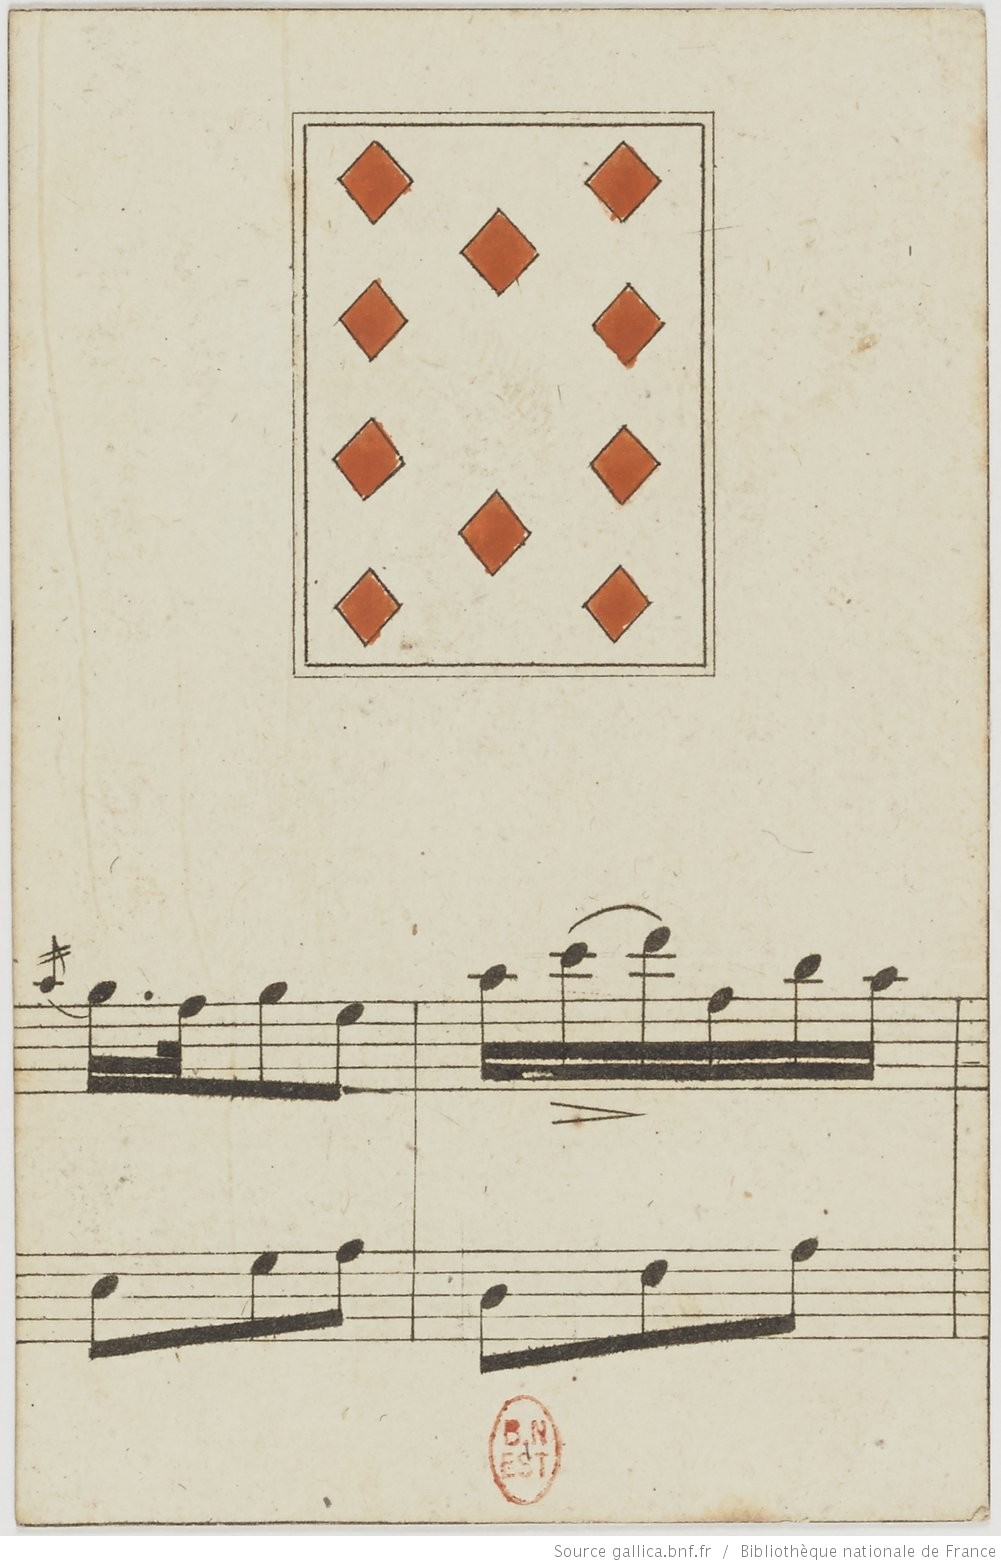
\includegraphics[height=5cm]{images/carte2.jpg}
\caption{\footnotesize Deux cartes d'un jeu de \guill{cartes musiciennes} de 1830, conservé à la Bibliothèque Nationale de France (auteur inconnu). Les mesures indiquées en-dessous des cartes sont conçues de manière à ce que le morceau formé par la juxtaposition de n'importe quelle suite ordonnée de cartes (As, Roi, Dame, etc., quelles que soient les couleurs choisies) soit une valse cohérente. Ce jeu forme ainsi un système de règles et a donc une nature algorithmique.}
\label{cartesajouer}
\end{center}
\end{figure}

C'est en 1984, qu'Essl utilise un ordinateur pour la première fois, par l'intermédiaire d'un ami, testeur pour un journal. L'année suivante, il investit dans un micro-ordinateur Atari ST, à sa sortie. Les années 1970 et 1980 correspondent à un changement radical dans les pratiques informatiques, qu'illustre cet achat. Alors qu'auparavant la logique de conception d'ordinateurs tendait vers des machines centralisées de plus en plus puissantes, apparaissent les \emph{micro-ordinateurs}, à usage individuels, qui vont progressivement s'imposer au détriment des premières. Le tableau \ref{micropc} montre quelques modèles emblématiques de cette tendance\footnote{D'après \cicite{Reimer,~2005} et \href{http://www.oldcomputers.net/}{http://www.oldcomputers.net/} (consulté le \today).}, caractérisée par une explosion à la fois des ventes et du nombre de modèles. Quant au tableau \ref{prixpc}\footnote{D'après \\ \href{https://web.archive.org/web/20091026193531/http://www.geocities.com/SiliconValley/Vista/3015/16bit.html}{https://web.archive.org/web/20091026193531/http://www.geocities.com/SiliconValley/Vista/3015/16bit.html} (consulté le \today).}, il montre que l'Atari ST était significativement moins cher que la plupart de ses concurrents, ce qui est l'un des facteurs de son succès. Il a aussi été particulièrement populaire parmi les pionniers de la musique informatique du fait de son interface MIDI (norme définie deux ans plus tôt, pour un format de représentation informatique des données musicales) intégrée. L'acquisition de ce micro-ordinateur par Essl s'inscrit donc pleinement dans la tendance historique de cette période. Comme nous le verrons dans les parties suivantes (\ref{ircam} et \ref{liberte}), l'idéal de liberté associée à cette individualisation de l'ordinateur jouera aussi un rôle important dans la suite du parcours d'Essl. Philippe Breton la décrit ainsi : \guill{L'invention du micro-ordinateur \tpp~avait pour objectif explicite de battre en brèche la centralisation et la possession des précieuses \guill{informations} par quelques privilégiés. La \guill{guérilla} micro-informatique \tpp~a été en grande partie à l'origine de la \guill{culture informatique}, partagée dans un large public et facteur de démocratisation de la vie sociale et du savoir.} ; il ajoute que \guill{Pour les générations nées dans les années soixante, informatique et liberté sont désormais synonymes.} \cicite{Breton,~1987,~p.~206}.

\begin{figure}[!h]
\begin{center}
\begin{tabular}{|c|c|c|}
\hline
\textbf{Modèle} & \textbf{Année de lancement} & \textbf{Nombre d'exemplaires vendus} \\
\hline
Programma 101 & 1965 & 35.000 à 40.000 \\
\hline
%Intel MCS-4 & 1971 & §§§ \\
%\hline
Altair 8800 & 1975 & Quelque milliers \\
\hline
Apple II & 1977 & $\sim$ 2.000.000 \\
\hline
IBM PC & 1981 & Plusieurs millions \\
\hline
Macintosh & 1984 & $\sim$ 2.000.000 \\
\hline
%Amiga 1000 & 1985 & §§§ \\
%\hline
Atari ST & 1985 & $\sim$ 6.000.000 \\
\hline
Commodore 64 & 1982 & 17.000.000 à 25.000.000 \\
\hline
\end{tabular}
\caption{\footnotesize Quelques modèles de la naissance de la micro-informatique.}
\label{micropc}
\end{center}
\end{figure}

\begin{figure}[!h]
\begin{center}
\begin{tabular}{|c|c|c|c|c|c|}
\hline
\textbf{Modèle} & Commodore 64 & Atari 1040 ST & Commodore& Apple& IBM PC AT \\
&&& Amiga & Macintosh Plus & \\
\hline
\textbf{Prix} & 595\$ & 999\$ (mono) ou & 1795\$ & 2195\$ & 4675\$ \\
& & 1199\$ (couleur) & & & \\
\hline
\end{tabular}
\caption{\footnotesize Prix des micro-ordinateurs les plus répandus en 1985}
\label{prixpc}
\end{center}
\end{figure}

Sur son Atari ST, Essl programme d'abord en BASIC (\emph{Beginner's All-purpose Symbolic Instruction Code}), un langage de programmation impératif généraliste conçu pour sa simplicité d'utilisation. Il se tourne ensuite vers un langage beaucoup moins répandu, le LOGO\footnote{Plus précisément le xLOGO, l'une des nombreuses implémentations du langage original. Pour plus d'informations sur le LOGO, voir \cicite{Harvey,~1985}.}. Celui-ci a été développé à partir de la fin des années 1960, à l'origine par deux chercheurs du MIT, Seymour Papert et Marvin Minsky. Les programmes écrits en LOGO dirigent le déplacement d'un curseur représentant une tortue ; leur résultat est un dessin, celui de la trajectoire de la tortue. Cette apparence ludique est due au fait que le LOGO, conçu en s'appuyant sur les théories de Jean Piaget, était destiné à permettre à des enfants de se familiariser avec la programmation ; il s'agit cependant d'un langage très complet qui permet par exemple de manipuler des fichiers ou des structures de listes. C'est principalement cette dernière fonctionnalité qui retient l'attention d'Essl, lequel implémente des procédures issues du sérialisme. Essl développe en LOGO une bibliothèque, intitulée \emph{COMPOSE} (1988-), c'est-à-dire un ensemble de fonctions qu'il peut utiliser dans la composition de diverses pièces.

La pensée algorithmique devient prépondérante dans les œuvres du jeune compositeur. Sa première pièce ayant nécessité un programme informatique, \emph{BWV 1007a} paraît en 1986 (en collaboration avec son ami Eckel). Le programme était conçu pour réaliser une analyse statistique de la \emph{Première suite pour violoncelle} de Jean-Sébastien Bach (BWV 1007, 1720), afin de la découper et recombiner ensuite, de sorte que cette recombinaison soit mélodiquement cohérente. Précisons que cette expression peut être trompeuse : lorsque l'on parle de programmes et d'algorithmes, il est facile de laisser imaginer une \guill{volonté} ou une forme de conscience de l'ordinateur. Il n'en est évidemment rien, le programme d'Essl ne fait en réalité qu'exécuter des instructions prévues par lui. Une recombinaison \guill{mélodiquement cohérente} signifie ainsi simplement une recombinaison respectant des règles définies par Essl dans le but d'éviter des combinaisons sonores qu'il juge incohérentes. En cela, \emph{BWV 1007a} est un bon exemple de ce qu'est --- et donc de ce que n'est pas --- un algorithme : Essl aurait théoriquement pu appliquer lui-même sa méthode, découper et recombiner la pièce de Bach, en s'assurant de respecter les règles mélodiques qu'il a prévues ; mais cette tâche aurait été particulièrement fastidieuse ; l'ordinateur permet de l'automatiser et de la réaliser plus rapidement. La même année, Essl compose l'une de ses premières œuvres majeures, le quatuor à corde \emph{Helix 1.0}, qui lui vaut deux prix en 1987, au concours international de quatuors à cordes de Budapest et au concours    de quatuors à cordes du Konzerthaus de Vienne. Cette pièce construite sur des structures élaborées représentant des mouvements en hélice (comme combinaison de deux mouvements, l'un circulaire, l'autre rectiligne) reflète une véritable pensée algorithmique\footnote{Encore une fois, il y a deux causes à cette présente structurante forte des algorithmes : l'influence de la programmation informatique qui occupe Essl à cette période, mais aussi l'omniprésence de procédés d'ordre algorithmique dans la tradition musicale.}. Les algorithmes impliqués ont cependant été réalisés sans l'aide de l'ordinateur.

Il faut noter que l'attirance pour la musique algorithmique est totalement emblématique de cette période. Tous les compositeurs ne s'intéressent pas à l'informatique ---~l'une des caractéristiques de l'art depuis le \XXe~siècle est le nombre et la pluralité des écoles concurrentes --- mais c'est une tendance forte dans le milieu musical. Tendance marquée par le développement d'\emph{environnements informatiques de composition}, des logiciels, dont certains offrent les fonctionnalités de langages de programmation graphiques, qui simplifient la tâche de conception algorithmique des compositeurs. Ces environnements se multiplient à partir du milieu des années 1980 ---~et leur amélioration ainsi que le développement de nouveaux environnements se poursuit jusqu'à aujourd'hui --- : \emph{Autobusk} en 1986, \emph{Music Box} en 1986, \emph{HMSL} (\emph{Hierarchichal Music Spectification Language}) et \emph{Voyager} en 1987, \emph{Finale} en 1988, \emph{Cubase} et \emph{Common} en 1989\dots

Pour un compositeur qui a accordé aux aspects algorithmiques de la composition une place prépondérante dans son œuvre, Essl a une relation inhabituelle aux algorithmes. Sa position est résumée par cet échange dans une interview de 2015 : \guill{Magdalena Halay : Qu'est-ce qui pour vous fait qu'une composition sonne algorithmique ? --- Karlheinz Essl : Oh, le but n'est pas que mes compositions sonnent algorithmiques ! \tpp~Le but est qu'elles ne sonnent pas algorithmiques.} \cicite{Essl~et~Halay,~2015}.
Les méthodes formelles impliquées dans le processus de composition d'Essl sont \emph{théorisées}, \emph{décrites} (dans des articles, des programmes accompagnant les performances ou leurs enregistrements, les cours et les interviews donnés par Essl\dots) ; mais elles ne sont pas \emph{audibles}, ou du moins de sont pas mises au premier plan lors de l'écoute. Cette attitude s'oppose à celle de beaucoup d'artistes contemporains ayant recours à des algorithmes, qui au contraire en font la monstration à travers leurs œuvres\footnote{On peut trouver de nombreux exemples dans \cicite{Wilson,~2012}, en particulier au chapitre 7 intitulé \guill{\emph{Algorithms}}, p.~160-179.}. Elle opère ainsi une sorte de synthèse entre l'esthétique de la virtuosité (du compositeur) et celle qui met les moyens de composition au service de l'expérience de l'auditeur.

%\zitat{Deshalb glaube ich, dass das Wissen darum für den Hörer nicht unbedingt nötig ist. Die Stücke sollten deshalb sinnlich, also ganz im Bereich des Klanglichen, rezipiert werden. In beiden Fällen gehe ich jedoch vom Hören aus: die Strukturgeneratoren (ob sie nun die Lexikon-Sonate, Amazing Maze oder Champ d'Action betreffen) gehen immer von Wahrnehmungsphänomenen aus, niemals von abstrakten oder gar mathematischen Prämissen. Deshalb meine ich auch, dass sich meine Musik am besten durch offenes, bereitwilliges und vorbehaltloses Hören erschließt, in einem aktiven Wahrnehmungsprozess, in dem sich der Hörer aufgrund seiner jeweiligen persönlichen Voraussetzungen sozusagen seine eigene Fassung der Komposition mitkomponiert. Hören wird hier nicht zum bloßen Abbilden und Entziffern einer vorgegebenen Wirklichkeit, sondern zu einer schöpferischen Konstruktion.}
%{Karlheinz Essl / Bernhard Günther - Realtime Composition - Musik diesseits der Schrift} §§§

% Berlioz l'opposition §§§ : \guill{L'accent expressif d'une composition musicale n'est ni plus puissant, ni plus vrai, parce qu'elle est écrite en canon perpétuel, par exemple ; et il n'importe à la beauté et à la vérité de l'expression que le compositeur ait vaincu une difficulté étrangère à leur recherche}. Mémoires http://maxencecaron.fr/wp-content/uploads/2010/11/Memoires_Berlioz.pdf

Ainsi, les dernières années d'études d'Essl, qui sont aussi ses premières années en tant que compositeur, marquent ainsi l'apparition et le développement dans sa pensée artistique de pratiques algorithmiques. Ce phénomène va de pair avec celui de l'avènement de la micro-informatique, qui permet à Essl d'expérimenter avec sa propre machine. Il élabore alors une articulation relativement originale entre le procédé algorithmique et son résultat esthétique. Comme nous allons le voir dans la partie suivante, les progrès technologiques vont lui permettre d'enrichir encore grandement cette originalité.

\subsection{IRCAM et Composition en temps réel}
\label{ircam}

Un tournant décisif dans l'histoire de la musique informatisée et dans la carrière d'Essl a lieu à la fin des années 1980 et au début des années 1990. Il s'agit de l'apparition de dispositifs en \guill{temps réel}\footnote{Ce que recouvre exactement la notion de temps réel en musique est discuté plus précisément dans la partie \ref{tempsreel}.}. Ceux-ci offrent pour la première fois la possibilité d'une interaction immédiate entre l'utilisateur et une machine \emph{informatique}\footnote{La nouveauté réside dans le fait que c'est avec un ordinateur, une \emph{machine à calculer}, que le temps réel est obtenu : en musique électronique, les synthétiseurs permettaient ce temps réel depuis plusieurs décennies\dots~et les instruments de musique traditionnels, depuis toujours.} qui convertit le résultat de ses calculs en événements musicaux significatifs, typiquement sous forme de sortie MIDI (ce qui permet de produire du son avec des instruments comme le Yamaha Disklavier\footnote{Piano mécanisé créé en 1987 ; la norme MIDI a quant a elle été établie en 1983.}) ou directement dans un format audio (écouté \emph{via} des haut-parleurs).

\begin{figure}[!h]
\begin{center}
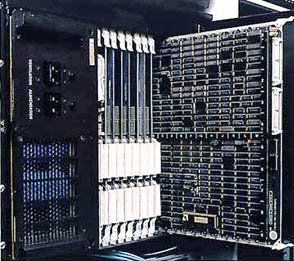
\includegraphics[height=5cm]{images/sim1.jpg}~~
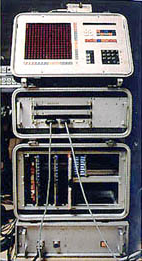
\includegraphics[height=5cm]{images/sim2.jpg}~~
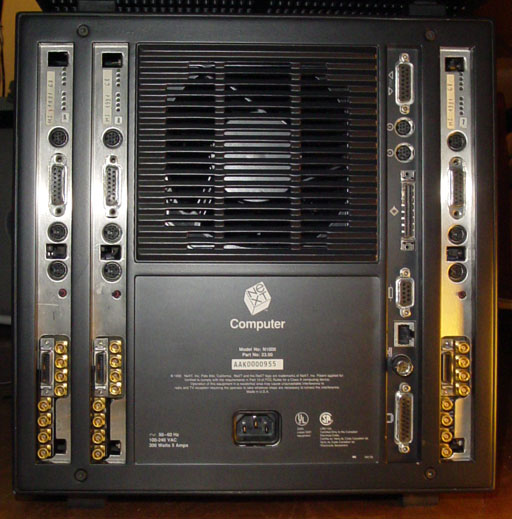
\includegraphics[height=5cm]{images/sim3.jpg}
\caption{\footnotesize Trois photographies de composants de la \emph{Station d'informatique musicale} de l'IRCAM. Il s'agissait d'un dispositif reliant plusieurs machines (ordinateurs, cartes son, claviers, interfaces) qui occupait une pièce entière. \copyright~Jean-Bernard Emond.}
\label{simphoto}
\end{center}
\end{figure}

Essl est confronté avec ces dispositifs en temps réel pour la première fois en 1992. Il est alors invité à l'Institut de recherche et coordination acoustique/musique (IRCAM) à Paris, institut public de création musicale et de recherche appliquée à la musique, qui lui passe commande d'une pièce pour ensemble et sa toute récente \emph{Station d'informatique musicale} (SIM)\footnote{Voir \cicite{Lippe~et~al.,~1991} pour une description détaillée de la station.}, visible sur la figure \ref{simphoto}. Cette machine succède à plusieurs autres prototypes développés par l'ingénieur et physicien italien Giuseppe di Giugno depuis 1975, intitulés 4A, 4B, 4C et 4X. Essl non seulement compose la pièce qui lui a été commandée (\emph{Entsagung}, 1991-1993), mais s'initie aussi au langage de programmation MAX avec lequel fonctionne la SIM, tirant profit de sa familiarité avec la programmation acquise au contact du LOGO pour réaliser des expériences de composition. Le \guill{temps réel} de l'IRCAM entraîne naturellement un gain de temps considérable, à travers deux ruptures. D'une part, les calculs sont exécutés plus rapidement : alors que les résultats des algorithmes de la bibliothèque \emph{COMPOSE} nécessitaient parfois une nuit entière de calcul, la SIM les calcule immédiatement. D'autre part, ces résultats sont audibles, c'est-à-dire dans un format directement intelligible ; lorsqu'il programmait en LOGO, Essl n'obtenait que des résultats sous forme symbolique (par exemple des nombres représentant des hauteurs de notes et leurs durées), qu'il devait ensuite traduire en partition et interpréter sur un instrument traditionnel.

La découverte des machines en \guill{temps réel} et de MAX est déterminante pour Essl, qui adopte les immédiatement comme des outils de travail de premier plan. Il transporte dans ce nouveau langage les algorithmes de \emph{COMPOSE} dans une bibliothèque intitulée \emph{Realtime Composition Library} (\emph{RTC-lib}), qu'il continue à enrichir et à optimiser. Il compose plusieurs pièces interactives en temps réel, parmi lesquelles son œuvre la plus célèbre, la \emph{Lexikon-Sonate}. La \emph{RTC-lib} et la \emph{Lexikon-Sonate} font l'objet respectivement des sections \ref{rtclib} et \ref{lalexikonsonate}.

L'interaction musicale en temps réel n'était cependant possible au début des années 1990 qu'avec les machines prototypiques conçues par des centres de recherche comme l'IRCAM, qui n'existaient donc qu'en nombre très limité. L'accès y était de fait difficile et concurrentiel ; en outre, Essl souhaitait composer en étant autonome de telles institutions. Il lui a fallu pour cela attendre 1998 et la sortie du premier iMac, suffisamment puissant pour obtenir des performances similaires à celle de la Station d'informatique musicale. Comme le montre la figure \ref{productivite}, cela coïncide avec un forte augmentation de sa productivité (en tant que nombre d'œuvres publiées).

\begin{figure}[!h]
\begin{center}
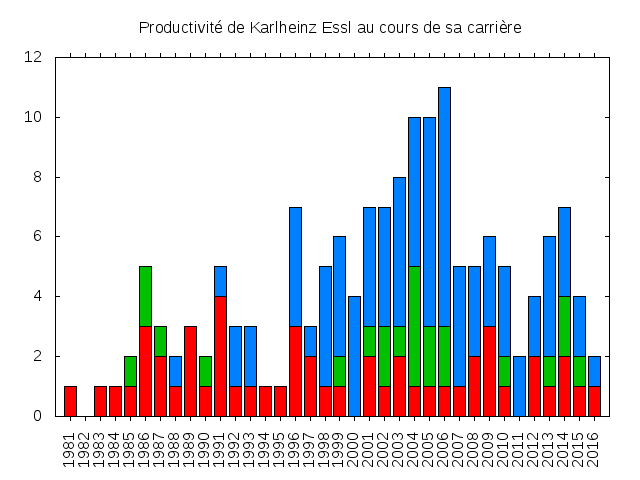
\includegraphics[width=12cm]{../Divers/plots/ComputerMusic3.png}
\caption{\footnotesize Graphique présentant le nombre de pièces produites par Karlheinz Essl par année. Les œuvres reportées en rouge sont des morceaux \guill{classiques}, celles en vert utilisent de la musique électronique mais seulement sous forme enregistrée, celles en bleu ont recours à la l'informatique pour leur exécution.}
\label{productivite}
\end{center}
\end{figure}

Ces œuvres d'une forme inédite sont le volet pratique du développement d'Essl, qui formule aussi de nouvelles notions sur le plan théorique, le conduisant à son rapport actuel à la musique algorithmique. Il élabore en particulier deux notions étroitement liées : celle de \guill{composition en temps réel} (\emph{Echtzeit Komposition}) et celle de \guill{\emph{Strukturgenerator}}\footnote{Littéralement, \guill{générateur de structure} ; dans ce qui suit nous conserverons le mot original.}. \\
Voici, pour les appréhender, deux définitions qu'Essl donne aujourd'hui des algorithmes : \guill{[Les algorithmes] sont le fondement de ma pensée musicale, qui consiste à ne pas voir la musique seulement comme une expérience sensible, mais comme quelque chose qui comporte une multitude de structures plus profondes que l'on peut exprimer sous forme de modèles.} \cicite{Essl~et~Hötzenecker,~2016}, et : \guill{Il y a la définition classique, qui provient plutôt des sciences de l'ingénieur, selon laquelle un algorithme est une sorte de recette de cuisine pour résoudre rapidement un problème. C'est une approche possible, mais il y en a une autre que je trouve plus intéressante. Elle consiste à envisager l'algorithme comme la définition d'un méta-modèle, duquel on peut obtenir différents résultats en modifiant les paramètres du système. C'est en ce sens que j'utilise le terme d'algorithme, et c'est ainsi que je le comprends dans les travaux de Gottfried Michael Koenig et Karlheinz Stockhausen.} (cité par \cicite{Förster,~2011}). \\
Essl fait aussi plusieurs fois référence à la notion d'\emph{Urpflanze} de Goethe, une plante originaire imaginaire dont on pourrait dériver toutes les espèces de plantes \cicite{Goethe~et~al.,~1993}. Le mot de \emph{modèle} est crucial dans l'idée de \emph{Strukturgenerator} \cicite{Essl,~1996}. Essl conçoit des algorithmes dont le produit peut varier selon les paramètres fournis en entrée et le hasard\footnote{Le rôle du hasard dans la composition en temps réel fait l'objet de la partie \ref{aspectsmateriels}.} interne des opérations exécutées par l'ordinateur, mais tout en respectant une structure imposée commune. Le module \emph{Triller} de la \emph{Lexikon-Sonate}, étudié dans la partie \ref{lsmodules}, est un exemple simple de \emph{Strukturgenerator}. Tout ce que produit ce programme a une \emph{structure} de trille : un ensemble de quelques notes répétées à grande vitesse ; mais les trilles générées par différentes utilisations varient par le nombre de notes différentes jouées, leurs hauteurs, la vitesse, la durée du trille\dots~L'idée de définir des éléments musicaux comme des représentants d'un ensemble des possibles gouverné par une structure, sous la forme d'un système de règles, n'est toutefois ni nouvelle ni originale. Les règles strictes gouvernant le contrepoint classique relèvent exactement de ce cas de figure ; la seule nouveauté dans les \emph{Strukturgeneratoren} d'Essl est qu'ils sont \emph{actifs}, l'ordinateur permettant de créer la musique à la demande une fois le système de règles explicité et traduit en code informatique. On retrouve des procédés similaires dans nombre de musiques algorithmiques où le temps réel n'est pas nécessaire, et beaucoup de domaines usent de tels schémas, par exemple dans les jeux vidéos où il est aujourd'hui monnaie courante de générer ainsi les décors. \\
En revanche, l'originalité d'Essl réside dans la manière d'utiliser ces \emph{Strukturgeneratoren} : ce qu'il nomme la \guill{composition en temps réel}. Celle-ci peut être décrite comme la conjugaison de la composition algorithmique avec le temps réel. Les pièces de l'œuvre d'Essl répondant à cette appellation peuvent être réparties entre deux catégories : les \emph{installations} et les \emph{méta-instruments}. Les installations sont des programmes qui génèrent de la musique sans intervention humaine, généralement utilisées dans un lieu précis comme à l'intérieur d'un musée. À la différence d'un simple enregistrement, le son émis par un programme de type installation est élaboré au fur et à mesure de sa diffusion. Ses caractéristiques notables sont en particulier l'absence de répétition, mais aussi de début et de fin en tant que tels. Les \emph{méta-instruments} sont des programmes offrant une interaction limitée (avec un \emph{instrumentiste}), mais dont le produit est du même type que celui d'une installation ; ce sont en quelque sorte des installations interactives dont un petit nombre de paramètres internes peut être modifié en temps réel. Un instrument traditionnel comme le violon laisse une liberté à celui qui en joue (hauteur, durée, volume des notes\dots), mais impose aussi certains paramètres du son (timbre, ambitus, nombre de notes pouvant être jouées simultanément\dots). C'est ce qui justifie cette appellation de méta-instrument, la principale différence étant que les instruments traditionnels sont déterministes (le même geste produira systématiquement le même son) mais généralement pas les méta-instruments programmés par Essl. Comme nous le verrons par exemple à travers l'étude détaillée de la \emph{Lexikon-Sonate}, c'est en combinant et associant des \emph{Strukturgeneratoren} qu'Essl réalise de tels programmes.

La spécificité de la composition en temps réel réside dans cette rencontre à la fois de la composition algorithmique et du temps réel, et représente une rupture qualitative par rapport à l'une et à l'autre. En effet, l'utilisation d'algorithmes n'était auparavant possible qu'en amont du moment de réalisation de la pièce. Quant aux technologies en temps réel, celles qui existaient déjà en musique électronique ne pouvaient être utilisées qu'en tant qu'instruments, pour produire et transformer du son. Les œuvres créées avec les prototypes d'ordinateurs en temps réel s'inscrivaient dans cette continuité, en utilisant la puissance de calcul pour élaborer de nouvelles transformations du son (par exemple \emph{Répons} (1981-1984) de Pierre Boulez ou \emph{Antara} (1985-1987) de George Benjamin). Essl a été l'un des premiers à mettre ces machines à calculer au service d'algorithmes de composition, et sans doute celui parmi ces pionniers qui a le plus approfondi cette notion. Par la suite, avec la démocratisation de l'informatique (tant matérielle que logicielle), les pratiques similaires se sont multipliées, avec par exemple l'apparition au début du \XXIe~siècle du \emph{live coding} (utilisation d'environnements de programmation interactifs pour \guill{improviser} des codes, écrivant ainsi devant une audience le code informatique générant la pièce entendue en même temps).

%\zitat{Le grand avantage du temps réel, ce n'est pas un gain de temps pour le compositeur --- au contraire cela représente une difficulté supplémentaire à maîtriser --- mais c'est qu'il intègre l'interprétation dans la musique électronique ; auparavant ces deux domaines restaient étrangers l'un à l'autre.}
%{La musique du temps réel, p. 44-45} §§§

%\zitat{Weil man sich beim Improvisieren nicht (wie beim Komponieren) "out of time" befindet, sondern mitten im Zeitablauf steckt, entstehen aus dieser Verantwortung und aus diesem Zwang heraus Situationen, die man als Komponist am Schreibtisch nicht planen kann.}
%{Improvisation über "Improvisation" - Karlheinz Essl \& Jack Hauser} §§§

%\zitat{+ description du processus de composition} §§§
%{Composing in a Changing Society - How does a composition come into existence ?}

Cette période est donc celle de la maturité pour Essl, celle où il affirme son style et définit son originalité. En découvrant le traitement informatique de la musique \guill{en temps réel}, et en s'en servant pour élargir la portée de ses travaux algorithmiques plutôt que de se concentrer sur le traitement du signal, il met au point la notion de \emph{composition en temps réel} qui sera sa marque de fabrique. C'est aussi la période où il prend totalement place dans le monde de la musique contemporaine. Ses études finies, il est invité à enseigner aux prestigieux \emph{Darmstädter Ferienkurse für Neue Musik} (cours d'été de Darmstadt pour la Nouvelle Musique) de 1990 à 1994, auxquels ont participé beaucoup des grands compositeurs du \XXe~siècle, en particulier germanophones (Adorno, Boulez, Cage, Stockhausen, Xenakis, mais aussi Luciano Berio (1925-2003), György Ligeti (1923-2006), Olivier Messiaen (1908-1992), Edgar Varèse (1883-1965)\dots) ; il devient ensuite professeur à l'université Anton Bruckner de Linz et donne des conférences dans de nombreuses universités à travers le monde.


\subsection{Descente de la tour d'ivoire}
\label{liberte}

Le dernier événement décisif dans le parcours d'Essl a lieu en 1997, lorsqu'il est invité au festival de Salzbourg (\emph{Salzburger Festspiele}) et présenté parmi les \guill{compositeurs de la nouvelle génération}. Le festival de Salzbourg, dédié à l'opéra, au théâtre et à la musique classique, est un événement de premier plan dans ces domaines. Il est de plus davantage tourné vers la musique historique (en particulier celle de Mozart, né à Salzbourg) que vers la création contemporaine ; l'invitation faite à Essl marque donc un sommet de sa notoriété de compositeur.

Cet aboutissement est cependant un coup d'arrêt pour Essl, que ces honneurs conduisent à prendre du recul et à interroger son parcours. Il décide alors de changer radicalement sa posture de compositeur, en quittant la \guill{tour d'ivoire} dans laquelle il travaillait jusqu'alors. Au lieu de seulement composer seul des morceaux (ou des programmes) et d'en confier l'exécution à des interprètes (ou des machines), il souhaite s'ouvrir vers le public et le reste du milieu artistique. Cela le conduit d'une part à devenir \emph{compositeur-performeur}, d'autre part à chercher à collaborer avec d'autres artistes pour ses créations futures.

Pour être à nouveau confronté au public, Essl devient donc \guill{\emph{performeur}}. La performance est une pratique artistique présente dans toutes les disciplines de l'art contemporain, supposant des actions éphémères à caractère unique\footnote{Au sens large, la musique générée par les programmes de composition en temps réel aurait donc un aspect performatif, au même titre que tout art de l'improvisation ; ce goût pour l'éphémère fait sans doute partie des motivations d'Essl à se tourner vers cette pratique et à la désigner ainsi.}, dont par exemple John Cage ou Yoko Ono (1933-) font partie des initiateurs. La désignation est cependant exagérée : les \guill{performances} d'Essl sont avant tout des improvisations. L'improvisation fait partie des terrains de jeu privilégiés de la création musicale contemporaine, comme en témoigne par exemple le compositeur américain George Lewis : \guill{[L'improvisation] se porte bien un peu partout. Beaucoup de monde essaie d'apprendre à improviser, parce que cela a toujours été un moyen formidable pour découvrir comment faire de la musique. Il y a une ébullition très intéressante parmi les improvisateurs --- de nouvelles manières de structurer, des idées élaborées pour intégrer des partitions à l'intérieur de l'improvisation, de nouveaux sons, un élargissement des notions d'\emph{instrument}, de \emph{virtuose}, et du rôle du performeur.} \cicite{Appleton~et~al.,~1986,~p.~81}.

La volonté d'Essl de jouer devant un public comme il l'avait fait avec les groupes de rock de sa jeunesse se heurte toutefois à un problème conséquent : il n'a aucun instrument dont il pourrait jouer. Bien qu'il ait comme nous l'avons vu joué du piano, de la guitare électrique et de la contrebasse, il n'a en 1997 plus aucune pratique instrumentale de haut niveau, et ne peut donc pas prétendre être ou devenir un instrumentiste de premier ordre. Là encore, il trouve la solution en capitalisant sur son savoir-faire informatique : \guill{Il serait difficile d'imaginer mon travail sans les ordinateurs, même lorsque je fais de la musique instrumentale ; c'est grâce à l'ordinateur que j'ai pu quitter ma tour d'ivoire} \cicite{Essl~et~Pagano,~2009}. Essl conçoit ainsi son propre \guill{instrument}, qu'il nomme \maze~(\emph{Modular Algorithmic Zound Environment}, 1999-). Programmer son propre instrument est une pratique commune dans la musique contemporaine. Le compositeur américain Curtis Roads témoigne ainsi : \guill{Beaucoup d'instruments digitaux peuvent être associés aux micro-ordinateurs de faible coût. La prolifération d'ordinateurs bon marché donne accès aux instruments intelligents à virtuellement n'importe quel musicien qui les souhaite.} \cicite{Appleton~et~al.,~1986,~p.~xviii}.

\begin{figure}[!h]
\begin{center}
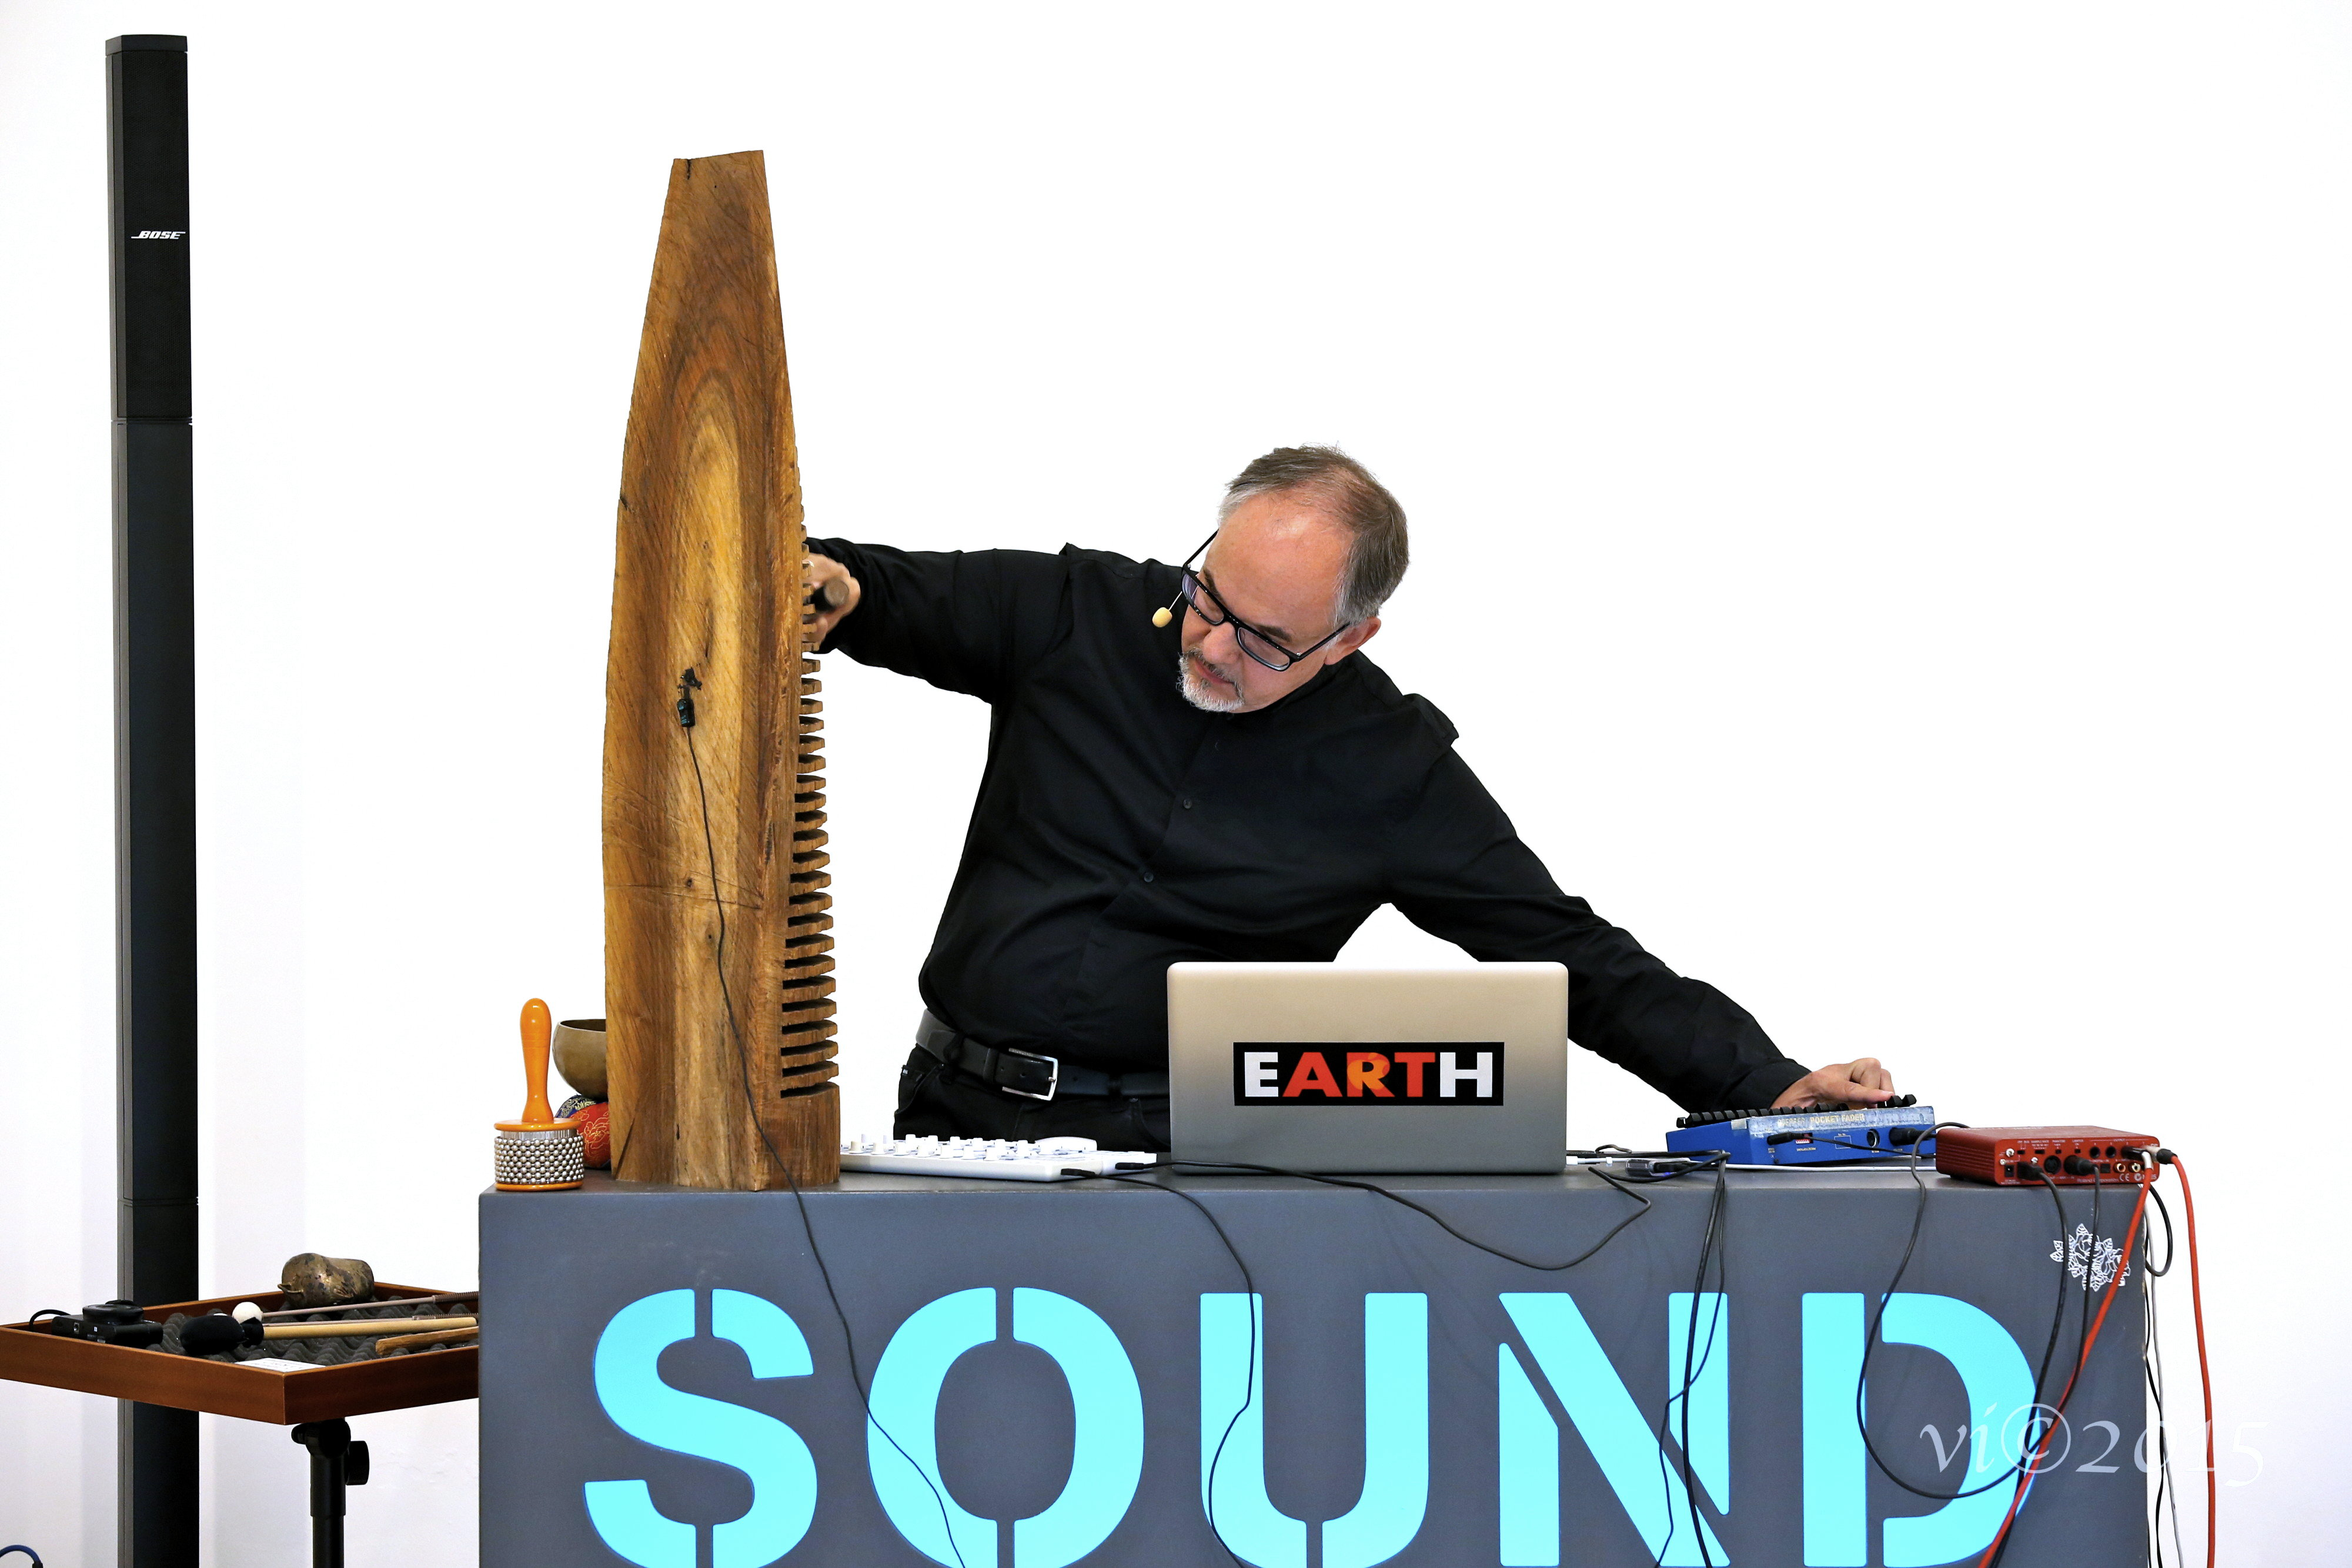
\includegraphics[width=10cm]{images/performance.jpg}
\caption{\footnotesize Karlheinz Essl réalisant une performance avec \maze~--- Photo \copyright~Viktor Br\'azdil}
\label{performancephoto}
\end{center}
\end{figure}

Comme on peut le voir sur la photographie \ref{performancephoto}, \maze~combine à la fois du matériel de musique électronique (pédales, micros, console MIDI\dots) et une interface logicielle. La partie physique, tactile, permet à Essl de mettre au point une sorte de \emph{geste} instrumental. Quant à l'interface logcielle, visible plus précisément sur la figure \ref{mazephoto}, elle incorpore des algorithmes de traitement du son et des \emph{Strukturgeneratoren} pour la composition en temps réel, manipulant ainsi des données sonores aussi bien que symboliques. Le \maze~est donc un méta-instrument dans le sens employé ci-dessus. On peut même parler de \guill{super-instrument}. Essl l'a en effet constamment développé et amélioré depuis sa création en 1998, y incorporant la plupart de ses créations logicielles. Le mot \guill{\emph{Modular}} dans son nom reflète le fait que le \maze~ne possède pas de structure contraignante ---~mais donc pas non plus d'unité --- comme un instrument au usuel (qu'il soit matériel ou logiciel). Il s'agit plutôt d'une collection de sous-programmes qui peuvent être exécutés séquentiellement ou en parallèle. Dans \emph{Machine Musicianship}, le compositeur contemporain Robert Rowe identifie \guill{trois classes d'algorithmes qui se prêtent particulièrement à l'interaction : le séquençage, la transformation et la génération. Le séquençage implique l'utilisation d'un matériau pré-enregistré qui est joué plus ou moins tel quel, mais où l'on contrôle les points d'entrée et de sortie, les boucles, la vitesse de lecture, etc. \tpp~Les techniques de transformation \tpp~prennent une source externe, lui appliquent une ou plusieurs transformations, et jouent ce matériau transformé en contrepoint de l'original. Les techniques de génération extraient un matériau de base d'un jeu de données fixe et lui applique des processus pour l'adapter, le prolonger ou l'embellir} \cicite{Rowe,~2004,~p.~203}. Ces trois classes sont présentes chez Essl. On voit en bas à droite de l'interface du logiciel (figure \ref{mazephoto}) que des extraits sonores pré-enregistrés sont présents, l'un d'entre eux étant entièrement représenté (en bleu), qui peuvent être séquencés grâce notamment au logiciel incorporé \emph{REplay PLAYer} (2000-2001), programmé d'abord indépendamment par Essl. La transformation est illustrée par la figure \ref{performancephoto}, où l'on voit qu'Essl se sert du \maze~pour augmenter\footnote{On parle en général d'\emph{instrument augmenté} lorsqu'un musicien ajoute des fonctionnalités électroniques à son propre instrument. La guitare électrique est un instrument augmenté.} des instruments traditionnels. Enfin, les \emph{Strukturgeneratoren} permettent la génération, dans le sens défini par Essl, plus large que celui de Rowe. Les modules de la \emph{Lexikon-Sonate}, dont deux sont étudiés dans la partie \ref{lsmodules}, sont par exemple intégrés dans le \maze. Cet instrument, qui rassemble la plupart des travaux du compositeur au cours de sa carrière, peut en somme être décrit comme une version condensée et ergonomique de sa table de travail, et destinée à l'improvisation.

On peut noter qu'en utilisant des \emph{Strukturgeneratoren} algorithmiques pour l'improvisation, Essl réalise là encore une synthèse dans une opposition classique, décrite par exemple dans \emph{Composers and the Computer} : \guill{[Tristan] Perich me dit que ses compositions émergent de l'improvisation, de l'esprit à l'œuvre --- en général le piano, qui est son instrument de prédilection. Il oppose ceci à d'autres compositeurs qui utilisent des algorithmes, ce qui entraîne des complications. \guilldeux{Il y a une différence entre un processus qui fait partie de l'inspiration ou de votre ensemble d'outils, et un processus qui fait office de déterminant.} Il préfère le premier.} \cicite{Appleton~et~al.,~1986,~p.~264}. Il y a bien, dans l'utilisation du \maze~pour l'improvisation, une composante \guill{hors du temps}, puisque les \emph{Strukturgeneratoren} du programme ont été conçus en amont de la performance (il ne s'agit pas de \emph{live coding}). Ce qui fait que la musique créée avec le \maze~reste improvisée, c'est que les algorithmes ne sont utilisés que localement, à la demande et sous le contrôle du performeur, et non pour décider de la structure générale de la musique.

\begin{figure}[!h]
\begin{center}
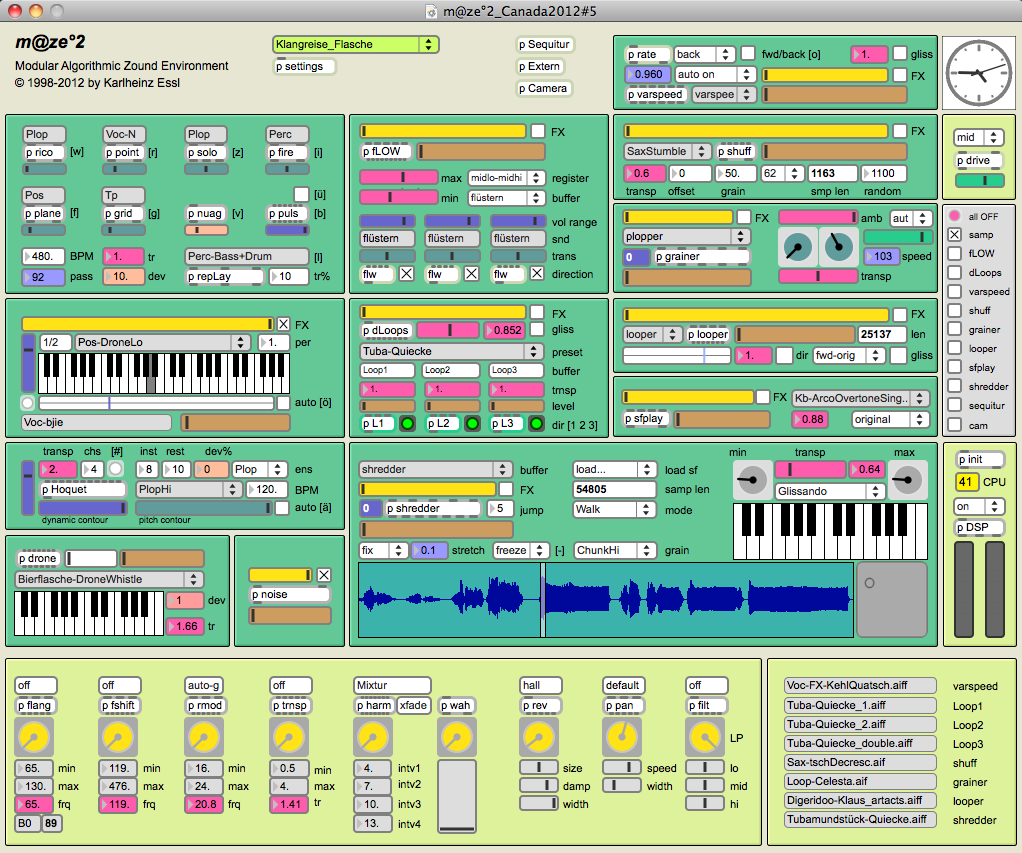
\includegraphics[width=9cm]{images/maze.png}
\caption{\footnotesize L'interface graphique du logiciel \maze~--- Photo \copyright~Karlheinz Essl}
\label{mazephoto}
\end{center}
\end{figure}

L'ouverture voulue par Essl passe aussi par la collaboration avec d'autres artistes, musiciens (instrumentistes et compositeurs) ou non. Cela l'amène à composer de nouvelles formes et pour de nouveaux cadres, comme l'écrit Julieanne Klein : \guill{La production musicale d'Essl couvre tous les media possibles : orchestre, musique de chambre, théâtre musical, performance, musique électronique \emph{live}, musique informatique et électronique, méta-compositions et compositions en temps réel, méta-instruments, installations et paysages sonores, musique de film, visuels, compositions textuelles et pièces pour instruments solo. Cherchant constamment à étendre sa production créative, Essl collabore fréquemment avec des artistes d'autres disciplines, y compris des chorégraphes, des danseurs, des plasticiens, des vidéastes, des architectes, des poètes, des écrivains, et des graffeurs.} \cicite{Klein,~2013}. L'abolition des barrières entre disciplines artistiques, et en particulier la sonification des supports visuels, est une tendance importante du champ artistique à partir de la fin des années 1980. C'est l'avènement du \emph{multimédia}, conséquence de la révolution numérique.

La concrétisation de cette nouvelle volonté d'ouverture passe par un projet d'envergure intitulé \emph{fLOW}. Il s'agit d'une entreprise polymorphe autour d'un programme homonyme générant un paysage sonore ; elle donne lieu à dix installations et vingt-deux performances (principalement en 1999 et 2000, mais les dernières ont lieu en 2007). Toutes incorporent le \maze, et chaque performance fait appel à des improvisateurs différents, jouant des instruments variés et issus de traditions musicales diverses (Nouvelle Musique, jazz expérimental, improvisation \emph{live}, musique électronique).

Enfin, un autre événement important se produit en 1999 : l'ouverture du Essl Museum. Elle apporte deux explications supplémentaires à la nouvelle orientation de la carrière d'Essl. D'abord, elle s'inscrit dans la même ligne idéologique : Karlheinz Essl senior a fait construire ce musée pour mettre sa collection personnelle d'art contemporain à la disposition du public\footnote{La motivation de ce projet n'est naturellement probablement pas seulement philanthropique --- sa vocation est en particulier sûrement aussi une entreprise de communication --- ; elle n'est du moins certainement pas économique, la construction du musée par l'architecte Heinz Tesar et son entretien étant assurés par le patrimoine de la famille Essl, sans aide publique. La mise à mal de ce patrimoine par la crise financière de 2007 à même conduit à un changement d'actionnaire majoritaire et à la fermeture du musée en juin 2016.}. Et sur le plan matériel, elle offre une plus grande autonomie à Karlheinz Essl junior. Celui-ci dispose en effet d'un studio à l'intérieur du bâtiment, et d'un poste de conservateur chargé de la programmation musicale, grâce auquel il peut mettre ses productions en scène à l'intérieur des expositions, et nouer des relations en organisant des concerts.

Cette dernière période est donc celle d'un changement de la pratique d'Essl, plus que dans son esthétique ou dans ses méthode de composition. À nouveau, ce tournant peut être mis en relation avec le contexte historique. Les progrès en informatique générale ont amené la musique numérique au grand public (les premiers baladeurs MP3 apparaissent ainsi en 1998), rendant obsolètes les travaux matériel en informatique musicale. Les institutions, dont le principal avantage outre la transmission de compétences entre compositeurs et musicologues était de rassembler les moyens pour le développement de ces prototypes, perdent en rayonnement. Les progrès en informatique musicale ne sont désormais presque plus qu'exclusivement logiciels.

\subsection{Conclusion}

Essl apparaît emblématique d'une génération. Les précédentes avaient connu la naissance de l'ordinateur, les débuts de la science informatique et les promesses de la cybernétique, la suivante est née dans un monde déjà informatisé ; celle d'Essl a vu les ordinateurs quitter les institutions pour conquérir la sphère privée, et s'imposer dans de nombreux champs de la société. L'informatique représente ainsi à la fois une réalité concrète, et un nouvel horizon à explorer, dont les progrès tangibles se font à de courtes échelles de temps. Elle a accompagné Essl tout au long de sa carrière de compositeur, qui lui a accordé une place de plus en plus importante dans son travail. Véritable moteur de son évolution, elle a guidé ses choix et permis de les réaliser, ainsi que de développer son originalité.

%\zitat{... with complete autonomy since without public funding
%... the famous names of 20th-century music with a clear inclination towards the composers that happily pursued the spirit of modernism even through the post-modern era. Hardly a coincidence, since kHz considers himself as belonging to that ilk.}
%{An Extended Composer’s Desk - Composer Karlheinz Essl as the music curator of the Essl Museum}



\section{Le rôle de l'informatique à travers ses programmes}

\subsection{Introduction}

Cette partie se propose d'analyser la manière dont Essl a recours à l'ordinateur dans sa pratique artistique. Cette analyse partira du code même des programmes qu'il a conçus, selon l'approche du séminaire \emph{Codes Sources}\footnote{Voir \href{http://codesource.hypotheses.org/}{http://codesource.hypotheses.org/} (consulté le \today).}, ainsi décrite par Baptiste Mélès, chercheur en philosophie spécialisé dans l'informatique : \guill{À celui seul qui prend la peine de les lire effectivement, les codes sources révèlent leur richesse. On y découvre que l’élégance d’un algorithme réside parfois hors de sa complexité, dans l’usage virtuose des idiomes du langage de programmation ou dans la connaissance fine de la machine à laquelle il est destiné. Bien souvent des codes sources comportent davantage de lignes de commentaires que de code. Tous ces trésors de pensée informatique fondent à la compilation comme neige au soleil. \tpp~Le but du séminaire est de décrire ces œuvres de l’esprit comme des textes à part entière.}

Nous commencerons donc par étudier les codes sources de deux créations majeures d'Essl : la bibliothèque \emph{Realtime Composition Library}, collection de fonctions écrites dans le langage MAX/MSP qu'il utilise dans la plupart de ses compositions informatisées depuis 1992, et la \emph{Lexikon-Sonate}, l'une des premières pièces écrites à partir de cette bibliothèque et le plus diffusé des programmes d'Essl. Cela conduira à discuter les notions, dont on verra qu'elles sont essentielles dans les travaux d'Essl, de \guill{hasard} et surtout de \guill{composition en temps réel}. Nous aborderons ensuite l'usage que le compositeur fait du réseau Internet. Pour finir, nous montrerons que les conclusions de ces différentes approches décrivent un rapport à l'ordinateur avant tout comme outil.


\subsection{La \emph{Realtime Composition Library}}
\label{rtclib}

La \emph{Realtime Composition Library} (\emph{RTC-lib}) est une bibliothèque, c'est-à-dire un ensemble de fonctions réutilisables dans des programmes, développée par Karlheinz Essl dans le langage MAX/MSP. Son développement commence dès 1992, c'est-à-dire dès le moment où Essl a été mis en contact avec ce langage développé un an plus tôt par Miller Puckette \footnote{Pour plus d'informations sur MAX, voir \cicite{Puckette,~1991} ; une brève description du langage est faite ci-après.}, lors de son stage à l'IRCAM. Son origine remonte même à 1988, si l'on considère qu'Essl a commencé par implémenter dans ce nouveau langage les algorithmes de composition qu'il avait déjà développés en xLOGO, rassemblés dans la bibliothèque \emph{COMPOSE}.

Cette bibliothèque est le socle de la plupart des œuvres réalisées par Essl impliquant la programmation. Il en recense 56 à ce jour : partitions, programmes, installations, \emph{works-in-progress}\dots, parmi lesquels certaines de ses créations majeures comme les \emph{Sequitur} (série de pièces pour divers instruments solo avec électronique \emph{live}, 2008-2010), \emph{fLOW} ou encore la \emph{Lexikon-Sonate}, étudiée dans la partie \ref{lalexikonsonate}. C'est aussi à partir d'elle qu'il a conçu l'\guill{instrument} qu'il utilise lors de ses performances, le \maze. Elle est distribuée sous licence libre : disponible en téléchargement, elle peut être utilisée et modifiée gratuitement, à la seule condition d'en citer les auteurs.

Dans ce qui suit, nous proposons, après une présentation générale du langage MAX/MSP, une description détaillée de cette bibliothèque, avec une classification de ses fonctions en deux catégories : les \emph{fonctions ergonomiques} et les \emph{fonctions compositionnelles}. On trouvera ensuite une analyse technique de ces fonctions mettant l'accent sur leur complexité, le type de pensée qu'elles révèlent ou encore la façon dont elles sont documentées, ce qui amène à dégager le projet esthétique qu'elles servent.

\subsubsection{Description}

\begin{figure}[!h]
\centering
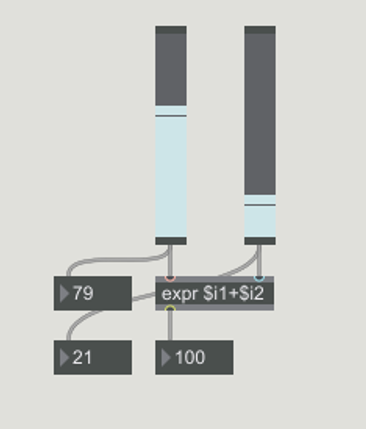
\includegraphics[width=5.5cm]{images/MAXbase.png}
\caption{\footnotesize Un programme basique en MAX/MSP : l'affichage et l'addition de deux entiers déterminés par des \emph{sliders}.}
\label{maxmsp}
\end{figure}

MAX/MSP est un \emph{langage de programmation graphique}, c'est-à-dire un langage de programmation dans lequel les programmes ne sont pas écrits en texte mais construits à partir d'éléments graphiques. Dans le cas de MAX, ces éléments sont des boîtes ou \guill{\emph{patches}} possédant des entrées et des sorties, et des liens qui permettent à ses fonctions d'interagir --- typiquement : relier une sortie d'un \emph{patch} à l'entrée d'un autre. La figure \ref{maxmsp} montre un exemple de programme simple. Ce type de représentation des programmes comme un assemblage de \emph{patches} reliés entre eux est la plus commune parmi les langages de programmation graphique, et on la retrouve dans d'autres environnements de CAO comme \emph{OpenMusic}. Il existe deux modes d'édition distincts, l'un pour construire le \guill{circuit} du programme, l'autre permettant de l'exécuter et de modifier les paramètres (valeurs numériques, impulsions ou \guill{\emph{bangs}}, curseurs, etc.). MAX ayant été développé expressément pour la musique assistée par ordinateur, il contient de nombreux \emph{objets} (fonctions) dédiés comme des entrées et sorties MIDI, ou consacrés au traitement du son\footnote{En réalité, MAX ne permettait à l'origine que la manipulation de données au format MIDI ; c'est la bibliothèque MSP, ajoutée en 1997, qui permet le traitement de signal audio (\emph{Digital Signal Processing}, ou DSP). Une autre bibliothèque d'importance nommée Jitter a été ajoutée en 2002, dédiée à la synthèse et à la manipulation graphiques.}.

\begin{figure}[!h]
\begin{center}
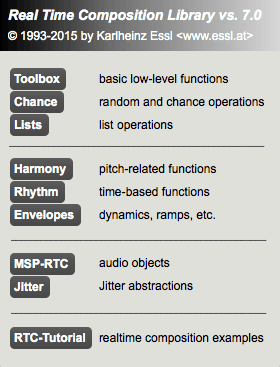
\includegraphics[width=4cm]{images/rtcmenu.png}
\caption{\footnotesize Le menu et les huit rubriques de la \emph{RTC-lib}. Photo \copyright~Karlheinz Essl}
\label{rtcmenu}
\end{center}
\end{figure}

La \emph{RTC-lib} compte à ce jour 177 objets en tout. 140 sont écrits par Essl, les autres en collaboration avec ou d'après d'autres compositeurs ou chercheurs\footnote{R. Albert Falesch, Charles Baker, Frank Barknecht, John Chowing, Chris Dobrian, Richard Dudas, Gerhard Eckel, Peter Elsea, Philippe Gruchet, Gary Lee Nelson, Serge Lemouton, James McCartney, Iain Mott, Eric Singer, Les Stuck et David Zicarelli.}. Elle est divisée en huit rubriques, qu'illustre en outre un tutoriel (voir figure \ref{rtcmenu}). Les trois premières rubriques, \emph{Toolbox} (outils divers), \emph{Chance} (opération aléatoires) et \emph{Lists} (traitement de listes), contiennent des objets \guill{basiques}. Les trois suivantes, \emph{Harmony} (gestion de hauteurs de notes), \emph{Rhythm} (gestion du rythme) et \emph{Envelopes} (gestion du volume), des objets \guill{de composition}, et les deux dernières, \emph{MSP} et \emph{Jitter}, regroupent les fonctions directement liées aux entrées et sorties son et vidéo. L'analyse qui suit propose un découpage différent. Les fonctions des rubriques \emph{Toolbox}, \emph{Lists}, \emph{MSP} et \emph{Jitter} seront appelées \emph{fonctions ergonomiques}. Elles répondent en effet au besoin de simplifier la tâche du programmeur en rendant plus rapides\footnote{Rapidité au moment de la création du code, pas de son exécution.} ou plus intuitives des procédures d'usage courant, qui pourraient aussi servir à la réalisation de programmes en-dehors de l'informatique musicale. Les autres rubriques regroupent les \emph{fonctions compositionnelles}, c'est-à-dire les fonctions qui résolvent des problèmes spécifiquement artistiques et musicaux. Aux trois rubriques qu'Essl fait entrer dans cette catégorie s'ajoute donc la rubrique \emph{Chance}.

\textbf{Les fonctions ergonomiques} \\
La plupart de ces fonctions sont très simples, en particulier dans la rubrique \emph{Toolbox}. On y trouve ainsi des fonctions réalisant les calculs de l'inverse d'un nombre, de son opposé, un accumulateur (fonction qui fournit la somme de toutes les valeurs qu'elle a reçues au cours de l'exécution du programme, ou le nombre de fois qu'elle a été appelée)\dots~D'autres corrigent ou améliorent des fonctions pré-existantes, comme la division euclidienne (qui ne fonctionne à l'origine que si le numérateur positif) ou l'arrondi (rendu paramétrable par Essl : au lieu de calculer seulement l'entier le plus proche de la valeur d'entrée, on peut arrondir à $x$ près).

C'est aussi le cas de la rubrique \emph{Lists}, dont la plupart des fonctions proposent simplement une forme plus ergonomique de fonctions pré-existantes. 14 d'entre elles se résument même à un renommage de fonctions contenues dans un objet nommé \emph{zl}. Celui-ci fournit de nombreuses procédures de manipulation de listes, mais aux noms peu explicites. \emph{Dans la RTC-lib}, \texttt{zl~rev} devient ainsi \texttt{reverse}, \texttt{zl~rot}, \texttt{rotate}, ou encore \texttt{zl~lookup} est légèrement modifiée pour devenir \texttt{nth}, qui renvoie le $n$-ième élément d'une liste fournie en entrée. La rubrique \emph{Lists} contient ainsi principalement des opérations simples et classiques sur les listes : calcul de la longueur d'une liste, de l'intersection de deux listes, scission d'une liste\dots~On en trouve d'autres qui résument en une seule fonction des opérations simples mais utiles et donc amenées à être utilisées souvent. Par exemple la fonction \texttt{butfirst} (respectivement \texttt{butlast}) cache simplement, en lui donnant une signification explicite, la scission d'une liste après son premier (respectivement avant son dernier) élément.

Enfin, les dernières fonctions essentiellement ergonomiques que contient la \emph{RTC-lib} sont des conversions, présentes dans chaque rubrique. Elles permettent au compositeur de manipuler les différents outils de la bibliothèque sans se soucier de leur compatibilité de type, qui peut être immédiatement gérée par ces convertisseurs. Cela va de transformations de \emph{pitch} (hauteur de note) en note au format MIDI ou en fréquence à celles entre différentes sorties sons, ou encore à celles entre durées relatives et absolues.

\textbf{Les fonctions compositionnelles} \\
Nous incluons la rubrique \emph{Chance} dans cette catégorie, parce c'est à notre sens dans celle-ci que réside le cœur de la partie véritablement compositionnelle de la \emph{RTC-lib}. En effet, les fonctions que que nous avons qualifiées d'\emph{ergonomiques}, bien qu'elles aient leurs spécificités et reflètent des partis-pris (comme l'importance accordée à la structure de liste), sont généralistes et répondent à des besoins d'abord \emph{techniques}. La rubrique \emph{Chance}, dédiée à la gestion de l'aléatoire\footnote{Ce que recouvre précisément la notion de \guill{hasard} en informatique est discutée dans la partie \ref{hasard}.}, rassemble comme elles des outils basiques et des fonctions simples utilisables dans d'autres contextes ; mais les utilisations possibles du hasard sont si nombreuses que les choix faits dans cette rubrique ont nécessairement une portée esthétique, sur laquelle s'appuient les modules \emph{Harmony}, \emph{Rhythm} et \emph{Envelopes}.

Plus précisément, elle rassemble principalement des générateurs aléatoires dont la variété rend possible une grande liberté dans le développement d'algorithmes musicaux. Là encore, l'ergonomie est une préoccupation centrale. Tous les générateurs sont ainsi déclinés en deux fonctions, selon qu'ils fournissent leurs résultats séquentiellement, ou directement sous la forme d'une liste. Là encore, toutes les fonctions ont un code relativement simple, parfois largement fondé sur des fonctions standard de MAX, comme la génération sérielle, présente nativement dans la fonction \texttt{xrandom} et rebaptisée \texttt{series}.

Les générateurs aléatoires présents dans la \emph{RTC-lib} implémentent des lois de probabilités classiques. On retrouve ainsi la probabilité uniforme (chaque événement possible a la même probabilité, comme sur un dé équilibré), sérialisme (la probabilité qu'un événement qui a déjà eu lieu se reproduise est nulle jusqu'à ce que tous les autres événements se soient produits chacun une fois), chaînes de Markov (déplacement sur un graphe donné, ou les probabilités de passage d'un état à un autre sont fixées à l'avance), mouvement brownien (aussi appelé \guill{marche aléatoire}, déplacement au hasard dans un espace donné tel que deux positions successives soient \guill{proches}). Certains de ces générateurs sont déclinés en plusieurs variantes intégrant des paramètres supplémentaires comme des pondérations ou des interdictions de répétition. On remarque aussi la présence moins commune de plusieurs générateurs reposant sur des échelles logarithmiques, ainsi que l'absence de générateurs reposant sur des distributions de probabilité comme les lois de Gauss ou de Poisson. D'une manière générale, on trouve presque exclusivement --- c'est-à-dire à l'exception du générateur de mouvement brownien, \emph{brownian} --- des générateurs \emph{discrets} et non \emph{continus}\footnote{Des générateurs dont les productions appartiennent à des ensembles prédéterminés et explicitement finis, par exemple les entiers entre $1$ et $12$, et non (théoriquement, l'ordinateur ne pouvant en réalité manipuler qu'un nombre très grand mais fini de données) infinis, par exemple l'ensemble des nombres réels $\mathbb{R}$.}. Les \guill{principes de sélection} de Gottfried Michael Koenig, dont la \emph{RTC-lib} et cette rubrique en particulier peuvent être considérées comme un développement, partagent avec elle cette particularité.

Dans les rubriques qu'Essl qualifie lui-même de compositionnelles, on peut distinguer trois sortes de fonctions : celles qui implémentent directement des méthodes classiques de composition, celles qui adaptent les générateurs aléatoires à cette fin, et les \guill{super-fonctions}. \\
Les premières fonctions sont ainsi spécifiques à la composition et au son, elles implémentent des comportements, des outils, des gestes classiques. Par exemple, la fonction $\texttt{neutral-harmony}(n,i)$ génère séquentiellement des notes à partir de $n$ par déplacement d'un intervalle $i$ puis de son complémentaire ; la fonction \texttt{metro-dev\%} modélise un instrumentiste humain en introduisant des approximations dans un battement parfaitement régulier ; la fonction \texttt{panning} calcule la distribution stéréophonique des volumes pour simuler le déplacement d'une source sonore. Parmi cette première sorte de fonctions, une sous-section entière de \emph{Harmony} (16 fonctions) est dédiée aux manipulations dodécaphoniques usuelles (génération de séries, calcul de l'inverse ou de la rétrograde d'une série, etc.). \\
La deuxième sorte de fonctions est une application des différents générateurs aléatoires (et de certaines opérations de listes) à chaque rubrique. Par exemple, la fonction \texttt{brown-melody} génère séquentiellement des notes dont l'enchaînement suit un mouvement brownien, sans répétition d'octaves. Sur le plan purement technique, ce sont à peu de choses près des convertisseurs qui transforment les résultats de ces générateurs en données représentant des hauteurs de notes (entiers représentant des \emph{pitches} ou \emph{pitch-classes}\footnote{Le terme \emph{pitch} renvoie à une hauteur de note au sens large, dans tout l'intervalle des fréquences audibles ; une \emph{pitch-class} est l'une des douze hauteurs de la gamme. Un \emph{pitch} correspond ainsi à l'association d'une \emph{pitch-class} et d'un \emph{registre}, qui indique dans quelle octave celle-ci se situe.}), des rythmes (émission de \emph{bangs}, ou entiers correspondant à des \emph{entry delays} (ED)\footnote{L'\emph{entry delay} d'un événement est le moment de son exécution dans la pièce, ou plus généralement la durée entre un point de départ global (comme le début du morceau ou d'une section) et le début de cette exécution.}), et des volumes (entiers entre $0$ et $127$). Néanmoins cette description est réductrice, en ce que ces fonctions, considérées de l'extérieur, possèdent un véritable contenu sémantique et dépassent de ce fait la simple conversion de données. \\
Enfin, les \guill{super-fonctions} combinent les précédentes. Elles n'apportent pas de possibilités créatives supplémentaires mais une interface pour choisir et alterner facilement entre les différents générateurs à disposition, en regroupant de plus de nombreux paramètres en entrée. C'est typiquement le cas du très complet \texttt{super-rythm}, visible sur la figure \ref{superrhythm}.

\begin{figure}[!h]
\begin{center}
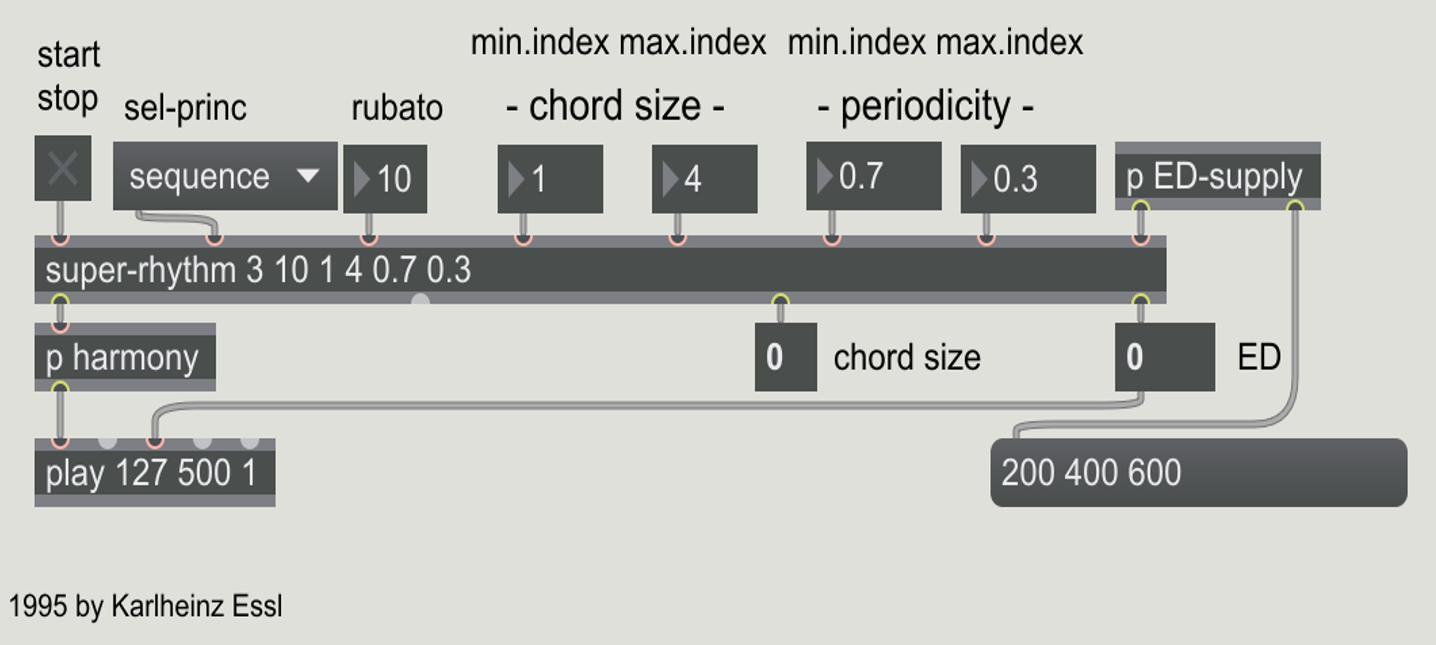
\includegraphics[width=\textwidth]{images/superrhythm.png}
\caption{\footnotesize La \guill{super-fonction} \texttt{super-rhythm}, qui génère un rythme de manière largement paramétrable. Les ED générés sont sélectionnés parmi une liste fournie en entrée (\emph{ED-supply}), selon un principe de sélectionau choix (\emph{sel-princ}, permet de sélectionner différents générateurs aléatoires). Une déviation aléatoire de ces valeurs d'origine peut être opérée (mesure par \emph{rubato}). Enfin il est possible de régler la taille des accords (\emph{chord size}, ou nombre de notes pouvant être jouées au même moment, donc au même ED) et la \guill{périodicité} (\emph{periodicity}), qui correspond à l'espérance mathématique du nombre de répétitions d'un ED immédiatement après avoir été sélectionné une première fois.}
\label{superrhythm}
\end{center}
\end{figure}


\subsubsection{Analyse}

L'analyse faite dans cette partie porte sur les aspects techniques et esthétiques de la \emph{RTC-lib}. L'analyse technique étudie les choix directement liés à la programmation et leurs conséquences, ainsi que le \guill{style} de conception de code. L'analyse esthétique montre le projet et les parti-pris artistiques que révèlent et servent ces choix techniques. Rappelons que les informations obtenues par ces analyses disparaissent à la compilation, c'est-à-dire lorsque le code source est transformé en programme exécutable. Les choix d'implémentation faits par Essl n'ont pas d'influence sur le produit de ses algorithmes, et \emph{a fortiori} sur la musique qu'ils génèrent ; ce sont sa pratique et sa pensée de programmeur qu'ils révèlent.

\textbf{Analyse technique} \\
Comme nous l'avons vu, la plupart des algorithmes présents dans la bibliothèque sont plutôt simples, mais il faut préciser ce que \guill{simple} signifie. La manière théorique de quantifier la complexité d'un programme informatique est d'évaluer sa \emph{complexité algorithmique}, qui correspond à l'ordre de grandeur du nombre maximal d'opérations élémentaires réalisées par une exécution en fonction de la taille de l'entrée\footnote{Pour plus de détails sur cette notion centrale de l'informatique théorique, se reporter à \cicite{Knuth,~1998}.}. Dans le cas de la \emph{RTC-lib}, tous les algorithmes ont une complexité \emph{constante} ou \emph{linéaire}\footnote{Exception faite de la fonction \texttt{sort}, réécriture de la fonction \texttt{zl sort}, qui trie une liste. Le tri est un problème algorithmique extrêmement classique, et les algorithmes qui le réalisent ont généralement une complexité de l'ordre de grandeur de $(n\cdot\log n)$ étapes pour une trier une liste de longueur $n$.}, ce qui est effectivement faible. À titre de comparaison, de nombreux algorithmes courants comme le calcul du plus court chemin entre deux points d'un graphe ont une complexité algorithmique strictement supérieure. Les algorithmes de complexité constante s'exécutent en un nombre constant d'étapes, quelle que soit la taille de l'entrée (ou alors la taille des entrées est bornée). Les algorithmes de complexité linéaire nécessitent un nombre d'opérations élémentaires du même ordre de grandeur que la taille de l'entrée. En outre, les portions complexes (linéaires, donc) des fonctions de la \emph{RTC-lib} ne sont jamais apparentes dans les \emph{patches} établis par Essl ; si c'était le cas, elles apparaîtraient sous forme de boucles ou de récursivité (une fonction récursive peut s'appeler elle-même avant de terminer son calcul), totalement absentes : les calculs sont effectués de manière directe, sans retour en arrière\footnote{Les seules traces de récursion apparaissent lorsqu'il faut interdire certaines valeurs en sortie d'une fonction (répétition, octaves). Dans ce cas un élément fait office de \guill{filtre}, teste si le résultat est valide et, s'il ne l'est pas, lance une nouvelle exécution du reste de la fonction jusqu'à finir sur une valeur autorisée. Ceci ne change pas significativement la complexité des fonctions concernées car la probabilité que les filtres doivent demander une nouvelle exécution est faible.}. Ainsi les seules sources de complexité sont cachées dans les sous-programmes (des fonctions natives) utilisés à l'intérieur des fonctions de la \emph{RTC-lib}, principalement les manipulations de listes et les objets de type \texttt{metronome}.

La pensée algorithmique que révèle la \emph{RTC-lib} est avant tout fonctionnelle. Cela signifie que le paradigme avec lequel Essl approche la programmation lui fait voir les algorithmes comme des fonctions qui \emph{calculent} (pensée fonctionnelle) plutôt que par exemple comme des listes d'instructions à exécuter (pensée impérative). La fonction \texttt{remove} de la rubrique \emph{Lists} illustre cette orientation : pour supprimer le $n$-ième élément d'une liste $L$, Essl calcule les sous-listes $L1$ et $L2$ séparées au niveau de cet élément, puis la liste $L1'$ comme $L1$ privée de son dernier élément, et enfin le résultat comme la jonction de $L1'$ et $L2$. Une pensée impérative aurait plutôt fait reculer d'un rang chaque élément à partir du $n+1$-ième. Que la pensée soit fonctionnelle n'a rien de surprenant car c'est la manière de programmer naturellement induite par le langage MAX, et associée avec l'utilisation de listes, omniprésentes dans la \emph{RTC-lib}\footnote{La structure de données équivalente, en programmation impérative, étant le tableau.}. Il est cependant intéressant de noter qu'Essl, qui a commencé à programmer avec des langages impératifs (Basic, LOGO\footnote{LOGO permet la création de fonctions, implémente la récursivité, utilise des listes, et repose sur un langage fonctionnel, le LISP ; sa philosophie générale est cependant plutôt impérative.}) maîtrise parfaitement les codes du paradigme de programmation le mieux adapté dans ce contexte --- malgré l'absence de récursivité, autre caractéristique essentielle de la pensée fonctionnelle.

Par ailleurs, les algorithmes sont généralement codés de manière directe, concise, et très claire. On peut même remarquer parfois le choix, augmentant cette concision, d'étapes \emph{hard-coded} : au lieu de faire calculer une sous-fonction de manière procédurale, l'ensemble de ses valeurs est intégralement décrit en donnée\footnote{Comme si par exemple une fonction calculant le carré de son entrée $x$, au lieu de calculer $x\times x$, retournait la valeur de la $x$-ième case d'une liste fournie au départ de la forme $1,4,9,16,25,\cdots)$. Dans la \emph{RTC-lib} ce \emph{hard-coding} est bien sûr utilisé pour simplifier des problèmes plus élaborés que cet exemple, par exemple pour calculer la distribution panoramique des volumes en fonction de la position supposée de la source sonore.}. Enfin, la documentation est très bien réalisée, avec des explications complètes mais claires de chaque fonction, l'organisation en rubriques, et la présence d'exemples ainsi que d'un tutoriel. Cette documentation, nécessaire à l'entretien du code à son appropriation par d'autre utilisateurs, tient à la volonté d'Essl de mettre effectivement cette bibliothèque à l'usage de tous.

L'analyse de la \emph{RTC-lib} montre ainsi qu'Essl programme d'une manière très bien adaptée au langage MAX. Il possède une maîtrise technique de son outil, adaptant ses compétence aux contraintes internes du langage de programmation qu'il utilise. L'efficacité de ses algorithmes et de la manière qu'il a de les présenter et documenter atteste en outre d'un savoir-faire plus général d'écriture et de diffusion de code informatique. Les fonctions de la \emph{RTC-lib} restent cependant très simples ; leur intérêt pour Essl réside dans la teneur musicale de ce qu'elles permettent de produire, et elles n'en ont aucun en tant qu'accomplissements techniques. 

\textbf{Analyse esthétique} \\
Il ne s'agit pas ici de faire une analyse esthétique approfondie, au sens courant, de la \emph{RTC-lib} en tant qu'œuvre d'art contemporain, mais bien de mettre au jour les parti-pris de l'artiste Essl sous-jacents aux choix d'implémentation du programmeur Essl.

La première influence très nette est celle de l'école sérielle. Elle transparaît naturellement dans les fonctions directement dédiées aux calculs sériels (générateur aléatoire sériel, fonctions dodécaphoniques). Mais elle se ressent aussi à travers l'omniprésence des listes, structure de donnée naturellement adaptée à la représentation de séries, qui structurent l'ensemble des moyens de stockage de la bibliothèque. On peut en outre relever l'influence directe de Gottfried Michael Koenig et de Karlheinz Stockhausen ; plusieurs algorithmes font des emprunts à leurs travaux et ils sont mentionnés dans les commentaires.

Par ailleurs, la représentation structurelle de la musique est très \guill{pianistique}. Les notes sont en effet décrites par uniquement une hauteur, une durée et un volume, ce qui modélise bien un piano mais pas par exemple un violon, dont le son résultant d'un seul geste musical peut évoluer dans le temps. Il aurait pu en être autrement compte tenu de l'intérêt qu'Essl accorde au son en général, mais cela n'a rien d'étonnant dans un langage de programmation qui privilégie la notation MIDI, et un langage musical marqué par la pensée sérielle.

Rythmiquement, on peut noter un affranchissement de la pulsation et de la notation sur partition, car ce ne sont jamais des noires, croches, doubles, etc., qui sont manipulées, mais exclusivement des durées absolues. Cette prise de liberté, qui s'associe à un rapport différent au temps de la musique est courante dans la musique du \XXe~siècle ; le compositeur Guy Reibel écrit ainsi : \guill{La pulsation disparaît au profit du voyage à l'intérieur de l'objet sonore, parcouru de son début à sa fin, lorsqu'il est formé, ou encore, plus radicalement, écouté hors du temps dans son écoulement et la variabilité de son flux lorsque sa durée est indéterminée \tpp~Le rapport au temps, à la notion de temps n'est plus le même, avec ces musiques qui \guilldeux{marchent toutes seules}, dans lesquelles l'homme a délégué son geste (celui qui produit le son) à la machine.} (cité par \cicite{Heinrich,~2003,~p.~89}). Enfin, lorsqu'il s'agit de générer les ensemble de valeurs parmi lesquelles opérer des choix aléatoires, Essl a une préférence nette pour les échelles logarithmiques, disponibles presque systématiquement. Ce choix traduit vraisemblablement la volonté de permettre à la fois précision et contrastes. % EXPLIQUER POURQUOI §§§

En conclusion, le projet esthétique qui s'appuie sur la \emph{RTC-lib} peut être qualifié de combinatoire. La bibliothèque est conçue comme une \emph{boîte à outils} plus que comme une collection d'algorithmes élaborés. Les fonctions qu'elle contient sont directes, et faciles d'utilisation ; elles sont techniquement simples mais très complètes, offrant une grande liberté de composition. La conception d'une œuvre avec la \emph{RTC-lib} passe ainsi par la combinaison de ces fonctions (à l'instar des modules de la \emph{Lexikon-Sonate}, étudiés dans la partie \ref{lsmodules}), et par le paramétrage des entrées qui peut engendrer des résultats musicaux très variés. Essl résume ainsi cette approche : \guill{La plupart des objets [de la \emph{RTC-lib}] sont orientés vers un traitement direct des données. L'utilisation de ces objets spécialisés rassemblés dans un \emph{patch} clarifie et simplifie la programmation. Beaucoup de fonctions qui servent souvent en composition algorithmique sont disponible dans cette bibliothèque --- ainsi le compositeur peut se concentrer sur la composition et non sur les aspects de programmation.} \cicite{Essl,~2010}.


\subsection{La \emph{Lexikon-Sonate}}
\label{lalexikonsonate}

La \emph{Lexikon-Sonate} (commencée en 1992 et continuée jusqu'en 2007) est la pièce la plus connue de Karlheinz Essl. Elle naît de la rencontre de deux projets. D'une part, Essl vient de découvrir MAX et d'importer les algorithmes qu'il avait précédemment développés dans ce qui deviendra la \emph{RTC-lib}. La \emph{Lexikon-Sonate} lui permettra d'expérimenter l'application en temps réel de ces algorithmes dans une pièce complète. D'autre part, un groupe d'artistes viennois nommé \emph{Libraries Of The Mind} conçoit un CD-ROM qui doit servir de support à un roman de l'auteur autrichien Andreas Okopenko (1930-2010), le \emph{Lexikon-Roman} (1983). Cet ouvrage présente la particularité de narrer un récit fictif sous la forme d'un dictionnaire au travers duquel le lecteur est invité à voyager. L'idée du groupe \emph{Libraries Of The Mind} est qu'il se prête particulièrement bien au format électronique, en tirant profit des liens hypertextes pour simplifier la lecture et les sauts d'une entrée à une autre. En outre, le projet propose d'enrichir le texte original en lui adjoignant des images et de la musique (faisant donc de ce CD un dispositif \emph{multimédia}). Essl est alors invité à composer de courts extraits ou paysages sonores, chaque entrée du dictionnaire devant être accompagnée par un échantillon. Il refuse néanmoins cette approche, estimant que la musique accompagnant le \emph{Lexikon-Roman} doit comme lui accorder une grande liberté au lecteur, par exemple changer nettement si celui-ci navigue rapidement d'une page à l'autre, ou au contraire conserver une ambiance stable si la lecture est calme.

C'est donc pour relever un double défi, technique et artistique, qu'Essl \guill{compose}, ou plutôt programme la \emph{Lexikon-Sonate}. Dans ce qui suit, nous allons décrire la pièce et les différentes utilisations qui en ont été faites, puis proposer comme pour la \emph{RTC-lib} une analyse d'une partie des algorithmes qu'elle emploie, et enfin dégager les conséquences que la forme de de la \emph{Lexikon-Sonate} entraînent pour l'œuvre et sa réception.

\subsubsection{Description}

\begin{figure}[!h]
\begin{center}
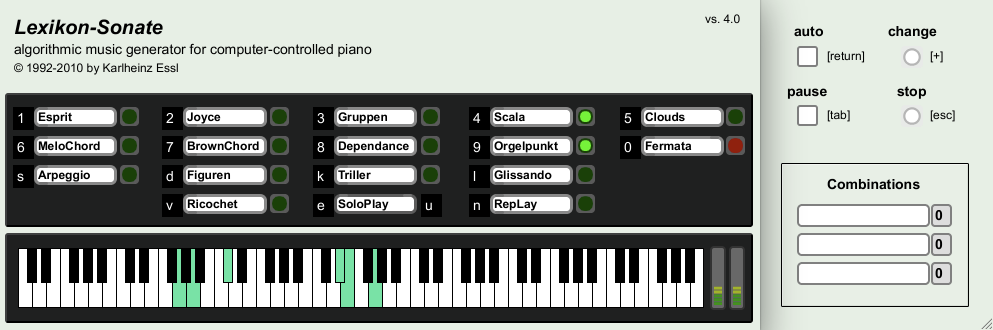
\includegraphics[width=\textwidth]{images/lexson.png}
\caption{\footnotesize Interface graphique de la \emph{Lexikon-Sonate}. Photo \copyright~Karlheinz Essl.}
\label{lsinterface}
\end{center}
\end{figure}

La \emph{Lexikon-Sonate} n'est pas un morceau au sens traditionnel du terme, mais un programme informatique qui génère de la musique. Reposant sur la \emph{RTC-lib}, elle utilise en temps réel des algorithmes de composition algorithmique pour générer de la musique au format MIDI, qui est alors ou bien directement convertie en son de piano de synthèse par l'ordinateur sur lequel le programme est exécuté, ou bien jouée par un piano mécanisé comme le \emph{Yamaha Disklavier}. Du fait de l'utilisation du hasard à plus ou moins grande échelle par les algorithmes implémentés en MAX par Essl, cette musique n'est ni prédéterminée ni prévisible, et se renouvelle donc sans cesse. Le programme génère donc à chaque exécution un morceau qui pourrait être sans fin, et se crée au fur et à mesure qu'il est joué sans jamais se répéter.

Comme on peut le voir sur la figure \ref{lsinterface}, la \emph{Lexikon-Sonate} utilise 17 \guill{modules}\footnote{Il en existe en réalité 24 en tout. Mais la figure montre la version libre de la \emph{Lexikon-Sonate} ; les 24 modules ne sont disponibles que dans une version plus complète qu'Essl réserve pour ses propres performances et celles d'artistes qui lui en font la demande.} (intitulés \module{Esprit}, \module{Joyce}, etc.) équivalents. Chaque module est un algorithme, construit en combinant des fonctions de la \emph{RTC-lib}. Ce sont ce qu'Essl nomme des \emph{Strukturgeneratoren} : le produit de chaque module respecte une forme, une structure préétablies. Les dites structures recouvrent une large variété de fonctions et de complexités musicales. \texttt{\textsc{Glissandi}}, qui génère des \emph{glissandi}, c'est-à-dire une série ascendante ou descendante de notes \guill{consécutives} (séparées d'un ton ou d'un demi-ton)\footnote{Il s'agit de la définition de la structure de \emph{glissando} telle qu'elle apparaît dans la structure de ce module, et non de la définition générale, plus large et recouvrant des réalités différentes selon les instruments. Dans le cas de la \emph{RTC-lib}, le format MIDI, essentiel dans MAX, impose au \emph{glissando} d'être discret, comme s'il était exécuté sur un piano. À l'inverse, le \emph{glissando} peut être envisagé comme \emph{continuum} de fréquences entre deux notes, comme celui que jouerait un violoniste. Cette approche est par exemple centrale dans la musique de Iannis Xenakis, et par conséquent dans l'environnement de programmation \emph{Iannix}, inspiré de ses travaux.}, est relativement simple à décrire, tandis qu'\texttt{\textsc{Esprit}} génère en théorie une mélodie \emph{expressive} au sens de la musique classique viennoise. Les différentes structures peuvent selon les modules s'apparenter à des mélodies, des accompagnements, des \guill{textures} ou des \guill{figures} ; certains comme \texttt{\textsc{Fermata}} sont même dédiés au silence, permettant à la musique composée de reprendre son souffle et de la segmenter, faisant entendre l'équivalent de parties et de sous-parties. Les programmes de deux de ces modules, \module{Triller} et \module{MeloChord}, sont étudiés en détail dans la partie suivante.

À chaque instant, exactement trois modules sont actifs. Ils génèrent chacun une séquence musicale correspondant à leur structure, de manière indépendante, qui sont jouées simultanément. Un changement des modules sélectionnés peut ensuite s'opérer (voir ci-dessous). La pièce jouée est ainsi la résultante du produit de trois \emph{Strukturgeneratoren} totalement autonomes. Pour conférer une unité auditive à cette superposition, qu'elle ne soit justement pas entendue comme une confrontation absurde de sons mais paraisse véritablement téléologique dans sa construction, les trois modules actifs reçoivent par ailleurs une pondération (\guill{premier plan}, \guill{second plan}, \guill{arrière-plan}), qui influence les paramètres réglant la gestion aléatoire du volume et de la proportion de silence. Essl affirme que les structures définies par les modules présentent des similarités avec des langages musicaux de l'histoire du piano, des \emph{topo\"i} de cet instrument, \guill{de Johann Sebastian Bach, Mozart, Beethoven, Schönberg, Webern, Boulez, [et] Stockhausen [à] Cecil Taylor}. Bien qu'il n'existe aucune citation directe des pièces pour clavier historiques, le programme est conçu de manière à ce que des formes musicales proches de celles-ci apparaissent au gré du hasard.

Il existe différentes manières de faire jouer le programme, autrement dit différents \emph{modes de jeu}. À l'origine, la \emph{Lexikon-Sonate} avait été imaginée comme une œuvre du type installation, avec une interactivité très limitée. La seule intervention possible de l'utilisateur était de provoquer le changement des modules actifs, qui s'opérait par remplacement du module présent depuis le plus longtemps, en suivant un principe sériel (après avoir été actif, un module donné ne sera plus réactivé tant que tous les autres modules n'auront pas été utilisés). Il s'agit d'une \guill{super-série}, puisque de nombreux modules utilisent aussi le principe sériel sur un niveau inférieur, et parce que son emploi pour combiner les modules n'a pas de conséquences facilement identifiables à l'écoute. Dans l'association originale avec le \emph{Lexikon-Roman}, c'est cette commande de changement des modules actifs qui permet de calquer les variations de la musique sur le rythme de lecture. Un mode de jeu alternatif, sans interactivité, est également implémenté, dans lequel les remplacements de modules s'opèrent à des moments déterminés de manière aléatoire.\\
Plus tard, Essl élargit le champ des possibles du programme et en fait un méta-instrument, en permettant à l'utilisateur de choisir lui-même quel module est activé et à quel moment. Cette version est distribuée librement en ligne ; dans une version plus élaborée réservée aux performances, le programme peut être relié à un contrôleur MIDI grâce auquel des paramètres globaux comme la \guill{densité} du son (proportion statistique de moments de silence) peuvent être réglés par l'interprète-performeur.\\
Ces différents modes de jeu sont autant d'approches de la nature combinatoire\footnote{Les propriétés combinatoires sont au cœur de nombreuses œuvres du \XXe~siècle, par exemple en littérature les \emph{Cent mille milliards de poèmes} (1961) de Raymond Queneau, recueil de cent quarante-vers pouvant être recombinés pour créer jusqu'à cent mille milliards de sonnets différents.} de l'œuvre. La grande variété du produit musical de la \emph{Lexikon-Sonate} repose en effet à la fois sur la variabilité à l'intérieur de chaque module et sur les très nombreuses possibilités d'association de ces modules (2024 agencements de trois modules distincts sont possibles, 12144 en prenant en compte les trois plans sonores).

Le choix du piano pour cette pièce n'est pas anodin. Essl parle d'une revanche envers un instrument qu'il n'avait pas aimé apprendre lorsqu'il était enfant
\footnote{\guill{L'un des points de départ est ma relation entre amour et haine avec cet instrument, le piano. À sept ans, j'ai été obligé d'apprendre le piano ; je voulais jouer de la flûte à bec. Je ne suis cependant jamais devenu bon pianiste. C'était toujours très frustrant de voir que j'étais incapable de mettre adéquatement en œuvre sur les touches ce que j'avais dans la tête. Bien sûr, mes premières recherches de compositions furent cependant des pièces pour piano, mais depuis je n'ai écrit aucun autre morceau pour le piano, et j'envisage difficilement d'en écrire à nouveau. Tout ce que je pouvais faire pour le piano, c'était une pièce qui obéisse à des critères absurdes.} \cicite{Ehrler,~1999}.} ; c'est d'ailleurs un instrument pour lequel il a relativement peu écrit\footnote{Outre la \emph{Lexikon-Sonate}, on recense seulement cinq pièces pour piano : \emph{Con una certa espressione parlante} (1985), \emph{Take the C Train} (2009), \emph{juncTions} (2011/2012), \emph{Gold.Berg.Werk} (2010-2014) et \emph{STERN} (2013). Et \emph{Take the C Train} est la seule autre œuvre pour piano solo (dans la mesure où l'on peut désigner ainsi la \emph{Lexikon-Sonate}).}. On peut dégager trois motivations à ce choix. D'abord, le projet d'associer la pièce au \emph{Lexikon-Roman} invite à adopter une démarche artistique proche de celle qu'il emploie. Or celui-ci est imaginé comme un pied de nez à la littérature classique, puisque le \emph{Lexikon-Roman}, c'est-à-dire le roman-dictionnaire n'est pas un roman mais bien un dictionnaire, qui contient cependant des références aux formes classiques. Le choix du piano permet d'évoquer l'histoire et le répertoire extrêmement riches de cet instrument ; le titre, \emph{Lexikon-Sonate}, ou sonate-dictionnaire, fait elle aussi allusion à la forme extrêmement classique de la sonate mais n'a évidemment aucun rapport avec elle dans sa construction. Elle ressemble de fait plus à un dictionnaire, avec cette banque de modules, qui permettent en outre à Essl de mettre l'idée de \emph{Strukturgenerator} à l'épreuve au travers de cette recherche de \emph{topoï} historiques. La deuxième raison est la justification du principe de superposition de trois modules simultanés. Comme le piano, ou plus généralement tout clavier, est l'instrument polyphonique traditionnel par excellence, sur lequel par exemple on \guill{réduit} les œuvres orchestrales lorsqu'un instrumentiste seul veut en faire entendre la teneur musicale, il est plus aisé d'écouter la rencontre de structures potentiellement contradictoires lorsqu'elle s'opère avec le timbre de cet instrument. Enfin, le piano est aussi l'instrument dont les modèles automatisés comme le \emph{Yamaha Disklavier} sont le plus répandus. Il s'agit par conséquent d'un choix naturel dans la conception d'une œuvre sous forme de programme contrôlant un instrument.

\subsubsection{Étude de deux modules : \textnormal{\module{Triller}} et \textnormal{\module{MeloChord}}}
\label{lsmodules}

Cette partie propose, comme ci-dessus pour la \emph{Realtime Composition Library}, une étude détaillée du programme de la \emph{Lexikon-Sonate}. Plus précisément, c'est \module{Triller}, l'un des \guill{modules} ou \emph{Strukturgeneratoren} qui composent la pièce, qui fait l'objet d'une analyse complète. Un autre module intitulé \module{MeloChord} est ensuite décrit de manière moins approfondie mais de façon à dégager les points communs avec \module{Triller}.

\textbf{Module~~\textnormal{\module{Triller}}} \\
Le module \module{Triller} est un générateur de \emph{trilles}. Traditionnellement, un trille est un ornement musical réalisé en alternant rapidement deux notes consécutives (séparées d'un ton ou d'un demi-ton). Cette définition est ici élargie : il s'agit d'un alternance rapide des notes d'un ensemble de 2 à 7 éléments, couvrant au plus une octave.

La figure \ref{trillermain} montre les deux parties principales du générateur de trilles\footnote{Les figures sont tirées des fonctions programmées par Essl en MAX/MSP. Précisons pour le lecteur qui souhaiterait les comprendre plus en détail que certaines liaisons sont masquées pour plus de visibilité. En outre, les \emph{patches} dont le nom commence par la lettre \texttt{s} (\emph{send}) ou \texttt{r} (\emph{receive}) font de même office de liaison : la valeur reçue par \patch{s label} est transmise à \patch{r label}. Enfin, les noms de \emph{patches} commençant pas \texttt{p} sont locaux : ceux-ci masquent un circuit complexe, mais le même nom utilisé à l'intérieur d'une fonction différente ne correspondra pas au même circuit. Par exemple, les deux \emph{patches} nommés \patch{p rhythm} dans les deux images de la figure \ref{trillermain} correspondent à des circuits différents. Ils sont seulement nommés ainsi pour indiquer que les circuits qu'ils représentent traitent tous deux d'aspects rythmiques.}. Il faut d'abord déterminer aléatoirement les différents paramètres du trille (quelles notes, à quel volume, etc.), et ensuite celui-ci peut être généré en temps réel. Il y a ainsi en quelque sorte un étape \guill{hors du temps}, la détermination des paramètres globaux, et une partie véritablement au fil du \guill{temps réel}, la génération de chaque note.

\begin{figure}[!h]
\begin{center}
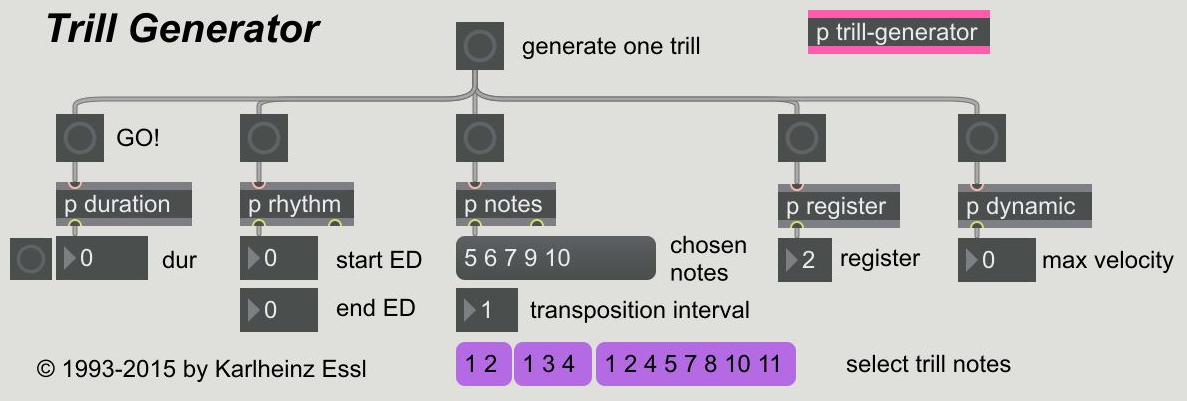
\includegraphics[height=4cm]{images/triller1.jpg} \\ \bigskip 
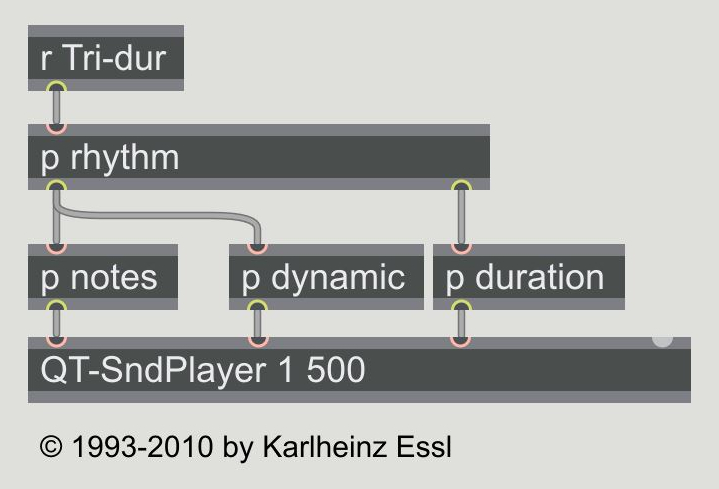
\includegraphics[height=5cm]{images/triller2.jpg}
\caption{\footnotesize Les deux parties principales du programme du module \module{Triller}. L'image du bas correspond à la génération des notes du trille en temps réel ; celle du haut regroupe les paramètres qui commandent celle-ci. Le circuit du haut est masqué par le \emph{patch} rose \patch{p trill-generator} de celui du bas.}
\label{trillermain}
\end{center}
\end{figure}

Comme on le voit sur la deuxième partie de la figure \ref{trillermain}, la génération des notes du trille est commandée en premier lieu par le rythme. La fonction \patch{p rythm} émet un signal à chaque moment où une note doit être jouée, qui active les fonctions \patch{p notes}, \patch{p dynamic} et \patch{p duration}, lesquelles déterminent chacune un paramètre (respectivement la hauteur, le volume et la durée) de cette note. 	Le synthétiseur \patch{QT-SndPlayer} reçoit ces informations et exécute la note correspondante. La subordination au rythme des autres paramètres du son dans l'ordre de détermination a d'importantes conséquences sur le processus de composition. Il est en effet plus compliqué ainsi de construire une ligne mélodique et de lui attribuer ensuite un rythme, par exemple de ralentir à la fin\footnote{Cela est plus compliqué ou moins évident, mais reste possible. Il faudrait placer le générateur mélodique en amont, qui fournisse son produit à la fois à une liste et au générateur de rythme. Les signaux émis par celui-ci commanderaient alors l'envoi progressif des notes de la liste au synthétiseur.}. Cette remarque montre que, bien que permettant en théorie de créer toutes sortes d'algorithmes (ne seraient-ce que tous ceux réalisables par un compositeur humain, sans ordinateur), les environnements de CAO sont des outils comme les autres, dont les contraintes orientent les parti-pris de leur utilisateur.

En tout, sept paramètres globaux régissent l'ensemble du trille produit, visibles en bas du premier circuit de la figure \ref{trillermain} : \emph{dur}, \emph{start ED}, \emph{end ED}, etc. Ici, ils sont déterminés lorsque le bouton central est activé, et dans la \emph{Lexikon-Sonate}, à chaque fois que le module est appelé. La durée totale du trille (\emph{dur}), les durées minimale et maximale entre deux notes successives (\emph{start ED} et \emph{end ED}, décidées par la fonction visible à gauche de la figure \ref{trillerf}), le volume maximum (\emph{max velocity}), l'intervalle de transposition (\emph{transposition interval}) et le registre (\emph{register}) suivent une loi de probabilité uniforme parmi l'ensemble de leurs valeurs possibles ; c'est la fonction \patch{between} de la \emph{RTC-lib} qui opère la sélection. Pour les trois premières, comme on peut le voir sur la figure \ref{trillerf}, les valeurs possibles sont réparties sur une échelle logarithmique entre les deux valeurs extrêmes, calculée par la fonction \patch{trans-log}. La détermination du matériel harmonique est plus élaborée, présentée à droite de la même figure. L'ensemble des notes de la gamme chromatique, représentée par les entiers de 1 à 12, est d'abord mélangé aléatoirement par la fonction \patch{scramble}. La fonction \patch{between} sélectionne uniformément le nombre de notes à conserver entre 2 et 6, et le transmet à la fonction \patch{slice} qui scinde adéquatement la liste mélangée. Le résultat est enfin trié par \patch{sort}. Cet algorithme permet effectivement de construire un ensemble aléatoire avec une probabilité uniforme (tous les produits possibles ont une probabilité identique). D'autres manières de parvenir au même résultat, y compris avec des fonctions de la \emph{RTC-lib}, étaient possibles, par exemple en choisissant des notes parmi les douze possibles selon le principe sériel. La méthode employée par Essl témoigne à nouveau d'une pensée fonctionnelle plutôt qu'impérative.

\begin{figure}[!h]
\begin{center}
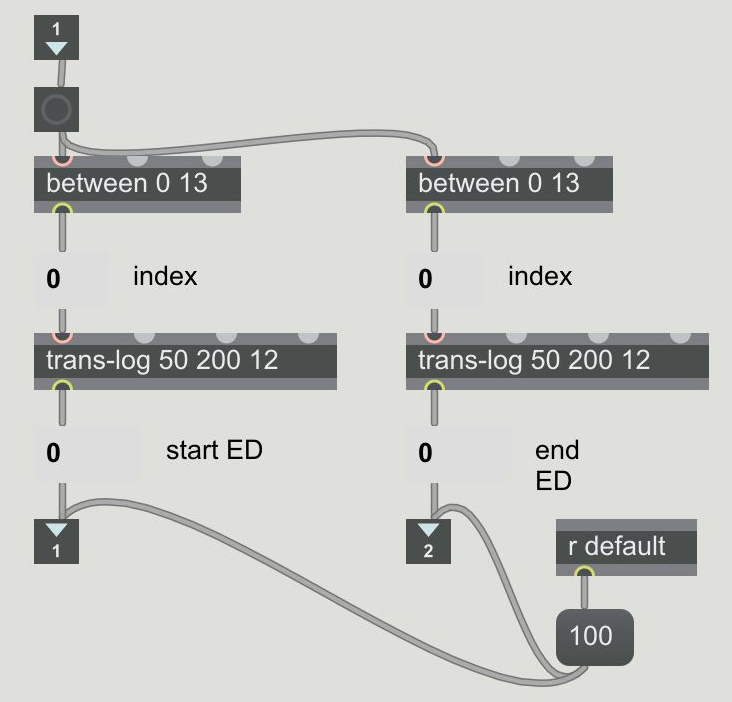
\includegraphics[height=6cm]{images/trillerED.jpg}~~~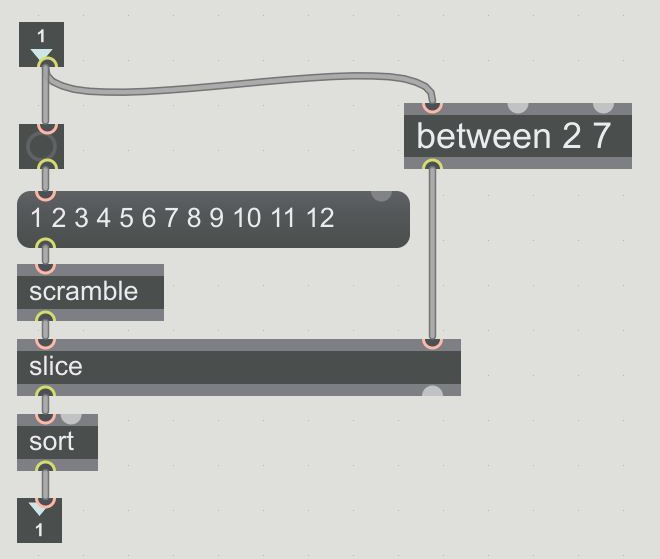
\includegraphics[height=6cm]{images/trillernotes.jpg}
\caption{\footnotesize Deux sous-circuits du module \module{Triller} utilisés pour la génération aléatoire des paramètres globaux. À gauche, on voit que les \emph{entry delays} (ED) minimal et maximal sont sélectionnés à l'intérieur d'une échelle logarithmique de 12 pas entre 50 et 200 millisecondes. À droite, c'est la sélection des notes du trille qui est opérée : mélange des entiers de 1 à 12 (qui représentent les douze notes de la gamme chromatique), récupération des 2 à 6 premiers, et enfin tri.}
\label{trillerf}
\end{center}
\end{figure}

Ces paramètres sont fixés pour tout le trille ; c'est à partir d'eux qu'est calculée chaque note. Certains des dits calculs utilisent des générateurs aléatoires. Le hasard intervient ainsi à deux échelles différentes dans le programme. Le rythme suit, à nouveau, une échelle logarithmique, ce dont il résulte un effet global de ralentissement. Cette échelle est calculée par la fonction \patch{ED-trans} de la \emph{RTC-lib}, afin que les durées entre chaque note varient de \emph{start ED} à \emph{end ED}, sur une durée totale de \emph{dur} millisecondes. À chaque signal rythmique, une note est générée. L'une des hauteurs pré-sélectionnées est choisie au hasard avec interdiction de répétition par la fonction \patch{permutate}. Elle est ensuite \guill{additionnée} aux deux paramètres \emph{transposition interval} et \emph{register} qui définissent la hauteur absolue de la note la plus basse du trille, et permettent donc à celui-ci d'être exécuté sur potentiellement n'importe quelle partie du clavier. Le calcul du volume sur l'ensemble du trille utilise la seule fonction \patch{schweller}, qui réalise un \emph{crescendo} suivi d'un \emph{decrescendo} entre le silence complet et le paramètre \emph{max velocity}. La durée de chaque note est aussi établie de manière déterministe, comme une fois et demie la durée qui la sépare de la suivante, ce qui donne un effet \guill{lié} au résultat entendu.

\textbf{Module~~\textnormal{\module{MeloChord}}} \\
Le module \module{MeloChord} génère des mélodies dont les notes peuvent éventuellement être enrichies par un accord. La figure \ref{melochordmain} montre que le principe d'organisation est identique à celui rencontré dans \module{Triller}. Un premier circuit génère les paramètres globaux de la mélodie, et un second crée celle-ci note par note, sous l'impulsion d'un générateur rythmique.

Ce module est visiblement plus complexe que le précédent, régi par douze paramètres différents. Il s'agit cependant d'une complexité \emph{horizontale}. Chaque génération de note implique plus de valeurs en entrée mais la profondeur du circuit est du même ordre de grandeur, et dans les deux cas il n'y a pas de boucle, comme dans la \emph{RTC-lib}.

À nouveau, les paramètres généraux sont majoritairement sélectionnés à partir de distributions uniformes, souvent parmi des échelles logarithmiques. Les hauteurs de notes utilisent des intervalles calculés par l'une des fonctions purement musicales de la \emph{RTC-lib}, \patch{choose intervals}, qui garantit des propriétés sonores du matériau généré (la somme de deux intervalles ne peut être une octave, on ne peut pas construire d'accord diminué d'après ces intervalles, etc.). Pour les paramètres de distances entre les notes (ED), de registre, et de durée (de chaque note cette fois, et non plus de la structure totale), on remarque la présence d'une option nommée \guill{périodicité}. Elle correspond à la probabilité pour chaque nouvelle note de conserver les valeurs de la précédente plutôt que de faire un nouvel appel au générateur aléatoire, afin d'obtenir par moments des unités sonores. Sur la figure \ref{melochordmain}, la \guill{périodicité} est élevée pour les notes courtes ($0.91$) et nulle pour les notes longues. Ainsi, lorsqu'une note courte est créée, il est probable qu'elle commence une phrase enchaînant des notes de même durée. D'une manière générale, le produit de ce module devant être plus varié que celui de \module{Triller}, il fait appel à plus de fonctions complexes de la \emph{RTC-lib}. La génération du volume fait ainsi appel à un mouvement brownien. Quant au générateur de rythme, il utilise la fonction \patch{repchord-rhythm}, qui dépend de six paramètres : les valeurs minimales et maximales d'ED, le nombre de pas pour l'échelle logarithmique calculée entre ces extrêmes, deux valeurs de \guill{périodicité} qui varie sur cette échelle, et la taille maximale des accords générés (autrement dit le nombre de notes qui peuvent être générées simultanément).

\begin{figure}[!h]
\begin{center}
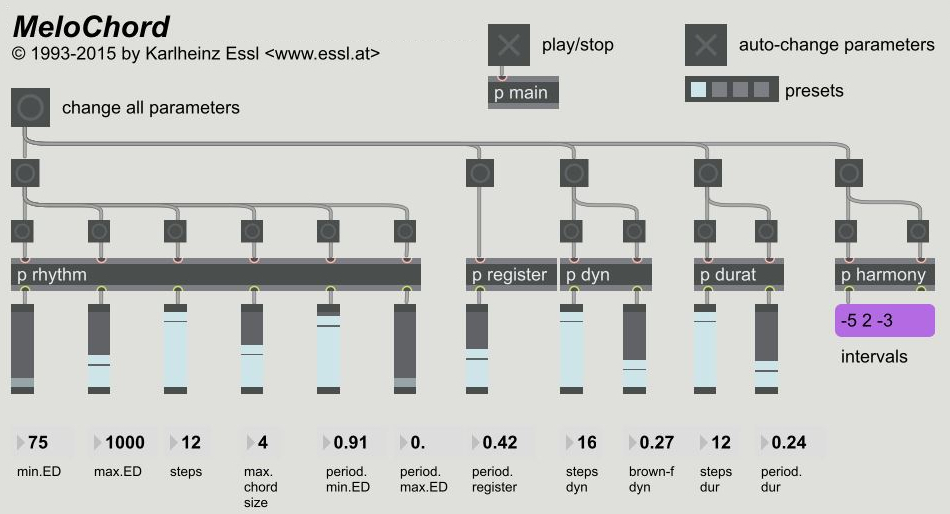
\includegraphics[width=12cm]{images/melochord1.jpg}~~~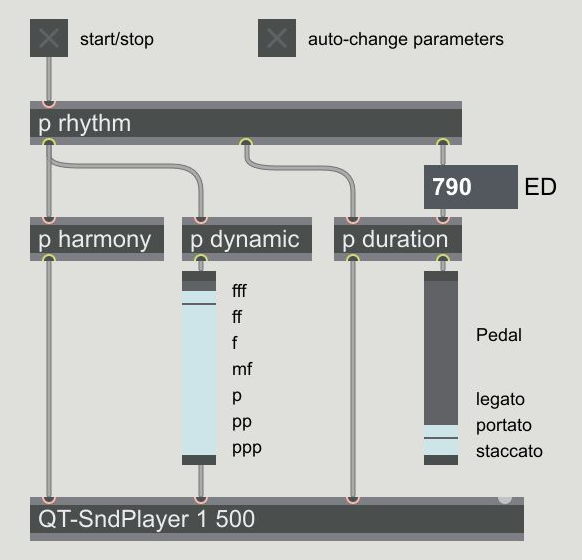
\includegraphics[width=5cm]{images/melochord2.jpg}
\caption{\footnotesize Les deux parties principales du programme du module \module{MeloChord}. L'image de droite correspond à la génération des notes en temps réel ; celle de gauche regroupe les paramètres qui commandent celle-ci. Le circuit de droite est masqué par le \emph{patch} \patch{p main} de celui de gauche.}
\label{melochordmain}
\end{center}
\end{figure}


\textbf{Conclusion} \\
Les principaux enseignements que l'on tire de l'étude de ces deux modules sont leurs similitudes dans la manière de programmer avec les fonctions de la \emph{RTC-lib}, la façon dont cette bibliothèque est utilisée selon une méthode généralisable, et l'importance accordée au hasard dans le langage musical.

Ainsi les conclusions formulées sur la \emph{RTC-lib} peuvent aussi s'appliquer à ces deux programmes de niveau supérieur. Les fonctions sont codées de manière directe, sans boucles sources de complexité, et commentées avec clarté. La pensée est principalement fonctionnelle, et traite le matériau musical avec des structures de listes. Bien que les deux modules soient relativement simples dans l'architecture de leur code, ils sont fortement paramétrables, ce qui permet de générer des résultats musicaux complexes et variés. La stratégie de genèse de ces modules n'est pas de suivre la logique du langage pour concevoir des structures mathématiques mais de faire obéir le code à des objectifs musicaux. On a de plus vu apparaître les contraintes inhérentes à l'environnement MAX/MSP qui ont incité Essl à subordonner au rythme les autres paramètres musicaux, montrant que, malgré les nombreuses nouvelles perspectives qu'elle ouvre et sa vocation universelle, la programmation possède comme tout outil technique des contraintes internes.

L'utilisation des fonctions de la \emph{RTC-lib} est effectivement un projet d'ordre combinatoire, et les générateurs aléatoires de la rubrique \emph{Chance} de la bibliothèque jouent un rôle fondamental. Chaque module repose sur un agencement de ces fonctions, dont l'intérêt ergonomique est exploité. Ils permettent en effet de donner un aspect intelligible à ces programmes, qui combinent les fonctions de la \emph{RTC-lib} comme celles-ci les fonctions élémentaires du langage. On remarque aussi que dans ces deux modules, les fonctions compositionnelles les plus complexes (en terme de variété des résultats) sont rares, mais que le processus de génération est organisé autour d'elles. Les fonctions plus simples comme le générateur uniforme \patch{between}, présent à de multiples reprises, les complètent, avec un impact moindre sur la complexité sonore de la musique créée.

Enfin, l'omniprésence du hasard montre que l'élément aléatoire est un lieu commun du langage musical d'Essl. Ce n'est plus une curiosité comme dans les jeux de dés musicaux, ni un enjeu comme dans la musique de Cage ou de Xenakis, mais un accessoire supplémentaire parmi les outils musicaux du compositeur. Le hasard est ainsi présent sur deux niveaux dans chaque module : d'abord pour sélectionner les paramètres globaux, ensuite pour la génération de chaque note. Une fois que les dits paramètres globaux sont fixés, le module répond à la définition de \emph{Strukturgenerator} puisque son produit respecte une certaine structure mais n'est pas prévisible ; pour le module complet, on pourrait donc même parler de \emph{Strukturgenerator} généralisé.

\subsubsection{Analyse}
\label{lsanalyse}

À nouveau, l'objectif de cette partie n'est pas de proposer une analyse esthétique approfondie de la pièce, mais de déterminer les spécificités d'une telle œuvre, en particulier dues à l'utilisation, d'une manière inédite lors de la création de la \emph{Lexikon-Sonate}, de l'outil informatique.

Essl explique\footnote{Voir entretien en annexe.} que la \emph{Lexikon-Sonate} est de par sa forme une sorte de métaphore de la vie humaine. Comme elle, elle est en perpétuelle évolution. Comme dans la vie humaine, des échos du passé y font régulièrement surface. Et de la même manière que l'être humain donne spontanément du sens aux nombreux événements et coïncidences qui se produisent en permanence, le principe de la pièce repose sur trois voix indépendantes mais dont la superposition doit faire croire à un réseau de sens. Naturellement, une telle métaphore est elle-même signifiante de la représentation du monde d'Essl\footnote{Il n'est pas anodin que cette \emph{Weltanschauung} à une époque où la science est dominée par la physique quantique, les lois du chaos et les systèmes complexes, soit gouvernée par des processus aléatoires, alors qu'à la période classique, où le monde était décrit comme régi par un Dieu omniscient et omnipotent, la musique obéissait à des contraintes formelles et thématiques très strictes. Ce parallèle est n'est toutefois qu'une ébauche dans la comparaison des représentations du monde historiques apportées par la science et l'art. On trouvera par exemple des remarques plus approfondies sur l'influence de la description scientifique du monde sur le champ artistique dans la première partie de \cicite{Eco,~1962}. Eco écrit par exemple : \guill{La propagation de certaines notions dans son milieu culturel [influence l'] artiste, au point que son art veut et doit être considéré comme la réponse de l'imagination à la vision du monde répandue par la science : \emph{l'art est une métaphore structurale de cette vision}} (p. 21).}.

La première caractéristique évidente de la \emph{Lexikon-Sonate} est qu'il s'agit d'une \emph{œuvre ouverte}. Cette notion assez large qualifie une œuvre dont certaines facettes ne sont volontairement pas maîtrisées ou arrêtées par l'auteur, mais laissées à celui qui la reçoit ou à des agents extérieurs --- en particulier, il s'agit généralement d'œuvres qui abandonnent l'idée d'un \guill{message} à transmettre au profit d'un champ d'interprétations possibles. La pièce \emph{4'33''} (1952) de John Cage est ainsi un exemple minimal et éloquent d'œuvre ouverte : elle consiste en quatre minutes et trente-trois secondes de silence de la part de l'interprète, tout en affirmant que chaque son produit dans la salle de concert pendant l'exécution de la pièce fait partie de celle-ci ; l'auteur est alors entièrement dépossédé de son œuvre qu'il soumet à la contingence des conditions de sa réalisation. Le concept est développé par Umberto Eco dans \emph{L'Œuvre ouverte}. Eco y fait remarquer que la définition peut être appliquée à n'importe quelle œuvre d'art, puisque la représentation mentale qu'elle induit chez celui qui la consomme varie d'un individu à l'autre, étant nécessairement soumise à l'interprétation. Mais nombre d'œuvres du \XXe~siècle se caractérisent par la mise en exergue de cette aspect intrinsèque de l'œuvre d'art. \\
Pour montrer que la \emph{Lexikon-Sonate} s'inscrit effectivement dans une problématique d'œuvre ouverte, nous allons mettre en avant trois caractéristiques essentielles d'une œuvre ouverte, que cette pièce possède effectivement : l'indétermination, la mise en retrait de l'auteur, et la remise en question de la notion même d'œuvre d'art. \\
L'indétermination, la place laissée à la contingence, est essentielle dans l'idée d'œuvre ouverte. Elle s'oppose en cela aux œuvres \guill{fermées} produites par les siècles précédents, c'est-à-dire les œuvres univoques, que critique par exemple Wittgenstein : \guill{Il me vient à l'esprit que dans les discours sur les objets esthétiques, on emploie des expressions telles que : \guilldeux{Il faut voir cela ainsi, c'est pensé ainsi}, \tpp~\guilldeux{Tu dois entendre cette mesure comme une introduction}, [etc.] (cela vaut aussi bien à propos de l'écoute que du jeu).} \cicite{Wittgenstein,~1953,~II,~xi}. Eco décrit la réponse suivante des artistes à cette critique : \guill{Aujourd'hui, l'accent est mis sur le processus, sur la possibilité de saisir \emph{plusieurs ordres}. Dans la réception d'un message structuré de façon ouverte, l'\emph{attente} implique moins une \emph{prévision de l'attendu} qu'une \emph{attente de l'imprévu}.} \cicite{Eco,~1962,~p.~105}. Il est clair que l'omniprésence de l'élément aléatoire, rendue possible seulement par l'ordinateur et une pièce sous forme de programme informatique, crée cet imprévu en permanence. \\
La mise en retrait de l'auteur, de l'artiste, qui renonce en quelque sorte à sa position de démiurge pour partager la paternité de sa production (typiquement avec le récepteur de l'œuvre, soit par l'interactivité, soit par l'interprétation dans une perspective proche du constructivisme radical cher à Essl), est un autre aspect important de l'œuvre ouverte. On pourrait la confondre avec l'indétermination ou du moins penser qu'elle est impliquée par elle, mais il n'en est rien. Si Essl avait construit sa pièce comme un unique \emph{Strukturgenerator}, sa position de créateur aurait été plus affirmée : certes le hasard déterminerait certaines modalités, mais l'auteur serait en mesure de décrire la structure de n'importe quelle exécution. Dans la \emph{Lexikon-Sonate}, le retrait est véritablement opéré par l'intrication des trois modules indépendants. À travers ce choix, Essl accepte l'impossibilité de prévoir même l'effet général produit par la pièce, et d'être lui-même surpris. Cette caractéristique, à la différence des deux autres étudiées ici, relève d'un parti-pris artistique et non de l'exploitation des nouvelles voies ouvertes par l'outil informatique. \\
Enfin, les propriétés de l'œuvre ouverte font qu'elle interroge la définition même de ce qu'est une œuvre. Adorno écrit ainsi : \guill{Contrainte par la logique de ses propres faits, la musique, en un mouvement critique, a dissous l'idée d'œuvre achevée et rompu avec le public. [\dots] Les seules œuvres qui comptent aujourd'hui sont celles qui ne sont plus des \guilldeux{œuvres}.} \cicite{Adorno,~1949,~p.~41-42}. Bien que ce ne soit pas si extrême dans le cas de la \emph{Lexikon-Sonate}, le fait qu'un programme informatique soit présenté comme un morceau de musique, renforcé par la référence à la forme historique de la sonate, questionne effectivement les délimitations traditionnelles de l'art. Elle affirme --- comme beaucoup d'autres créations contemporaines --- la possibilité de nouvelles acceptions de l'œuvre qui enrichissent la tradition artistique plutôt que de nécessairement rompre avec elle. \\

Une autre spécificité de la \emph{Lexikon-Sonate} découlant de sa forme informatique est l'absence de partition. L'enjeu de la notation a traversé toute l'histoire de la musique et trouve dans cette pièce un écho inédit. La partition classique, à l'origine très simple et conçue comme un simple aide-mémoire, a été sans cesse enrichie à travers les siècles, avec la volonté permanente d'une part de décrire de plus en plus précisément les paramètres d'interprétation, d'autre part de s'affranchir de ses contraintes (la notation du rythme sous formes de noires, croches, etc., est par exemple très contraignante). C'est pourquoi de nombreux compositeurs du \XXe~siècle ont élaboré de nouveaux systèmes de notation, comme Stockhausen qui en créait un spécifiquement pour chaque nouvelle pièce. La figure \ref{graphicalscore} propose quelques exemples de \emph{partitions graphiques} contemporaines.
Renoncer à la partition présente l'avantage de pouvoir explorer la musique sous un nouvel angle (typiquement pouvoir manipuler d'autres hauteurs de son que les seules douze notes de la gamme chromatique), mais revient aussi à renoncer à décrire l'œuvre ainsi créée d'une manière intelligible par n'importe quel musicien. Les conditions d'exécution sont alors beaucoup plus difficiles à réunir. Ce n'est pas le cas avec la \emph{Lexikon-Sonate}, dont la notation est le programme lui-même, qui présente l'avantage d'être un système simple et dépourvu d'ambiguïté pour son \guill{interprète} : l'ordinateur.

\begin{figure}[!h]
\begin{center}
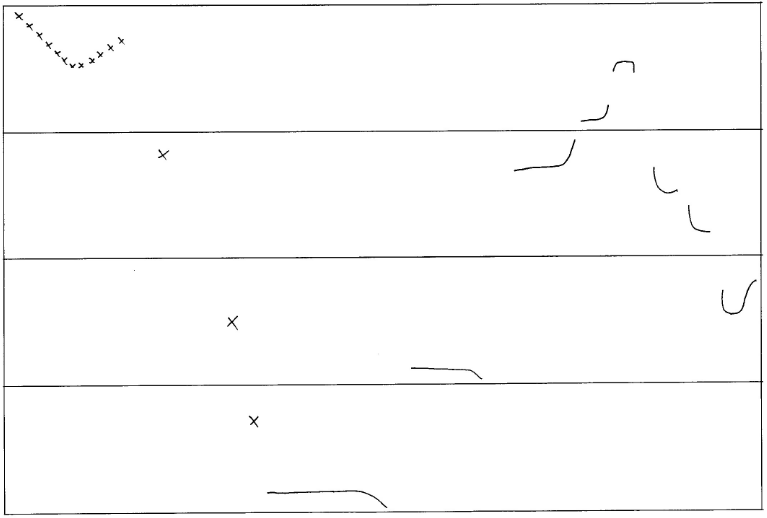
\includegraphics[width=5cm]{images/laonikos1.png}~~
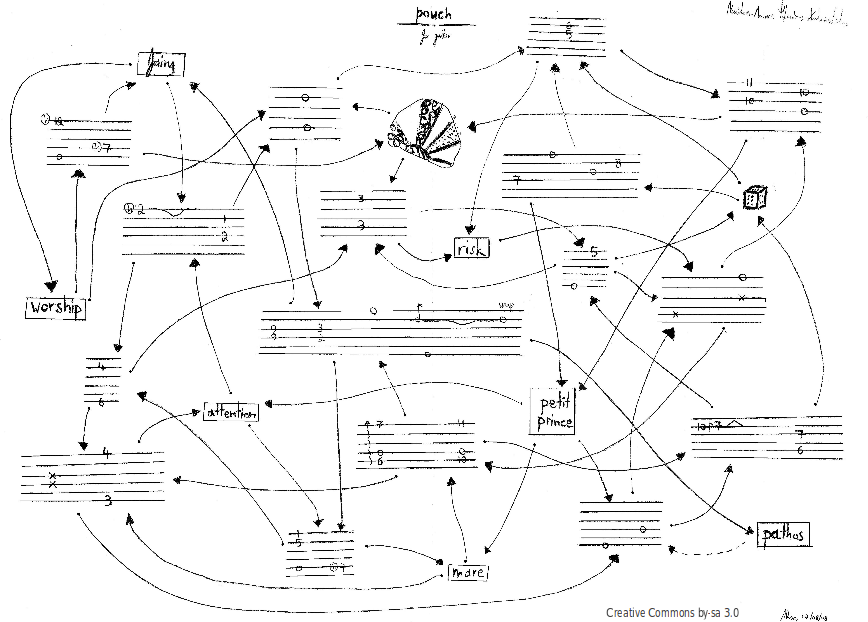
\includegraphics[width=5cm]{images/laonikos2.png}~~
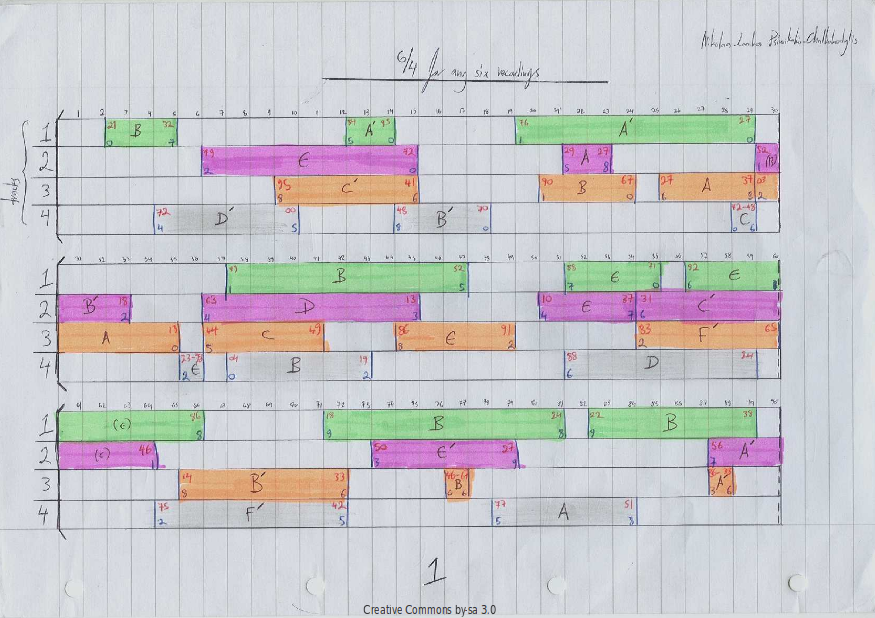
\includegraphics[width=5cm]{images/laonikos3.png}
\caption{\footnotesize Trois exemples de partitions graphiques, tirées des travaux du compositeur contemporain grec Psimikakis-Chalkokondylis (1989-), respectivement des extraits de \emph{Find the Sound} (2010), \emph{Pouch} (2008) et \emph{6-4} (2009). Ces partitions illustrent les nombreuses recherches des compositeurs à partir du \XXe~siècle de nouvelles façons de noter la musique. \copyright~Nikolaos-Laonikos Psimikakis-Chalkokondylis.}
\label{graphicalscore}
\end{center}
\end{figure}

Le fait que la \emph{Lexikon-Sonate} se passe d'interprète à d'autres conséquences. En particulier, la composition étant affranchie des contraintes de l'instrument, une nouvelle \guill{virtuosité} est possible. Par exemple, un pianiste humain ne peut jouer de \emph{glissando} que sur les seules touches blanches ou les seules touches noires. Dans la \emph{Lexikon-Sonate}, le module \texttt{\textsc{Glissandi}} généralise complètement cette définition en générant n'importe quelle suite monotone de notes séparées d'au plus un ton. De même, la figure \ref{partitionls} montre un extrait de la musique générée par le programme telle qu'elle pourrait être reportée sur une partition traditionnelle. Dans les deux cas, le résultat n'est pourtant pas complexe à l'audition ; simplement, la musique peut être déterminée grâce à des modèles qui n'ont plus à tenir compte des limitations physiques de l'instrument et de l'interprète. Cette liberté dans la composition n'est bien sûr pas spécifique à cette pièce ni nouvelle. Elle est permise par la machine mais ne nécessite pas le temps réel. La nouveauté que l'on trouve ici est à nouveau la synthèse opérée par la composition en temps réel : la composition algorithmique permet de prendre une partie de la responsabilité du compositeur, l'automatisation (de même que tous les procédés d'enregistrement) permet de se passer d'interprète, et dans l'exécution de la \emph{Lexikon-Sonate}, tous deux sont absents. En outre, cela permet de rendre infini ce qui ne pouvait être auparavant que fini. Lorsque la composition nécessitait plus de temps que l'exécution, les pièces devaient être délimitées dans le temps. Ici, composition et exécution sont simultanées : c'est grâce à cela ---~et bien sûr au fait que l'exécution est confiée à une machine, qui \guill{ne se fatigue jamais}\footnote{\guill{Un ordinateur ne se fatigue jamais. Avec l'ordinateur, on peut mettre en scène une musique qui ne s'arrête jamais. Cela n'est évidemment pas possible avec des musiciens.} \cicite{Essl~et~Pagano,~2009}.} --- que la musique peut se renouveler perpétuellement.

\begin{figure}[!h]
\begin{center}
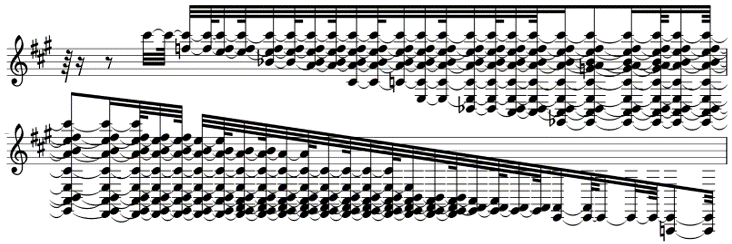
\includegraphics[width=12cm]{images/partitionls.png}
\caption{\footnotesize Environ deux secondes de musique jouée par la \emph{Lexikon-Sonate} transcrites sur une partition traditionnelle. Le son produit est simple (un arpège descendant avec les notes tenues), mais la partition paraît extrêmement compliquée. Cela est simplement dû à la liberté rythmique qui ne trouve pas d'équivalent dans ce système de notation.}
\label{partitionls}
\end{center}
\end{figure}

Enfin, cette redéfinition du schéma classique compositeur-interprète-auditeur a pour conséquence une nouvelle forme de sociabilisation\footnote{D'autres remarques sur les aspects sociaux du projet d'Essl, notamment à travers sa communication sur le réseau Internet, font l'objet de la section \ref{internet}.} autour de l'œuvre d'art. D'abord, grâce au caractère d'ouverture de la \emph{Lexikon-Sonate}, la hiérarchie entre l'artiste est son audience est en partie effacée. Essl écrit ainsi : \guill{Je veux mettre l'auditeur au défi de ne pas simplement consommer la pièce, mais tout en l'écoutant de devenir une sorte de co-créateur, un partenaire du compositeur et de la composition elle-même} \cicite{Essl~et~King,~1997}. Cette vision idéalise les faits : l'autorité du compositeur reste importante, mais l'auditeur est effectivement invité à approcher la pièce de manière plus active et ludique en tirant profit de l'interactivité (limitée) du programme. Cette interactivité oriente en outre vers une écoute \guill{savante}, ou du moins limite la possibilité d'une écoute véritablement naïve, puisque l'utilisation des appels de modules entraîne nécessairement une connaissance de base du fonctionnement de la pièce. Par ailleurs, l'absence d'interprète permet, comme la musique enregistrée, de diffuser plus facilement la \emph{Lexikon-Sonate}, et donc de toucher un public potentiellement plus large, d'autant plus que la pièce est proposée en téléchargement gratuit. Mais les différents auditeurs-utilisateurs auront chacun une expérience inévitablement différente, ce qui fait qu'ils auront moins en commun que s'ils avaient écouté la même musique fixée.

En conclusion, l'analyse de la \emph{Lexikon-Sonate} permet d'illustrer une application de la composition en temps réel, et ses conséquences : problématique d'œuvre ouverte, remplacement de la partition par le programme, libertés compositionnelles supplémentaires, nouvelle relation à l'auditeur. Les modules étudiés dépeignent la manière de programmer d'Essl, en combinant quelques fonctions de la \emph{RTC-lib} qui grâce au recours permanent au hasard deviennent des \emph{Strukturgeneratoren}, avec une recherche fondée davantage sur le résultat musical que sur la complexité des algorithmes.


\subsection{Aspects matériels du \guill{hasard} et du \guill{temps réel}}
\label{aspectsmateriels}

Cette partie aborde dans leur dimension technologique deux notions centrales dans les œuvres d'Essl : le hasard et le temps réel. Nous y expliquons comment l'informatique et \emph{a fortiori} l'œuvre d'Essl fait une approximation de ces deux phénomènes, suffisante pour ses besoins artistiques, et discutons les conditions historiques de l'apparition de la \guill{composition en temps réel}.

\subsubsection{Le \guill{hasard}}
\label{hasard}

Le hasard a comme on l'a vu une longue histoire dans le monde musical, bien que l'explosion de son utilisation n'ait eu lieu qu'au \XXe~siècle. Pour Essl, il s'agit par conséquent d'un élément déjà étudié et exploité par ses prédécesseurs, qu'il utilise donc comme une possibilité connue du langage musical plus que comme une nouveauté ou une curiosité.

La raison pour laquelle le hasard a pris une telle importance dans l'art de \XXe~siècle doit évidemment beaucoup à l'ordinateur\footnote{Mais pas seulement, John Cage ayant par exemple utilisé dans ses compositions de nombreuses opérations aléatoires manuelles.}, qui permet d'automatiser les processus aléatoires. Il n'est plus nécessaire de lancer des pièces ou des dés, il suffit de demander à l'ordinateur de générer un nombre aléatoire. Cette génération n'est cependant pas réellement aléatoire, car l'ordinateur n'incorpore aucun élément imprévisible comme le dé : il est entièrement déterministe. C'est pourquoi on utilise des générateurs dits \emph{pseudo-aléatoires}, dont l'histoire est aussi longue que celle des ordinateurs du fait des applications en cryptologie ; le premier de ces générateurs est ainsi mis au point par John Von Neumann (1903-1957), l'un des pionniers de l'informatique, l'année même de la mise en service de l'ENIAC, en 1946\footnote{Voir à ce sujet \cicite{Von Neumann,~1951}.}. Les générateurs pseudo-aléatoires sont des algorithmes qui génèrent des suites de nombres à partir d'une valeur initiale donnée, la \emph{graine}, qui paraissent être le fruit du hasard, ou possèdent des propriétés statistiques communes avec des expériences aléatoires. Le prochain nombre pseudo-aléatoire fourni par un générateur est imprévisible \emph{a priori} pour ses utilisateurs, mais qui a la connaissance de l'algorithme et de la graine peut le calculer, autrement dit le prédire avec certitude. Aux débuts de l'informatique, la génération \guill{rapide} de nombres pseudo-aléatoires était un véritable enjeu, mais que l'augmentation de la puissance des machines à calculer a très rapidement permis de dépasser en ce qui concerne leur utilisation dans le champ artistique.

La simulation du hasard est l'un des principaux attraits de l'informatique pour les compositeurs pionniers de l'informatique musicale, à partir de la fin des années 1950. Par exemple Koenig, qui utilisait déjà des processus aléatoires manuels dans ses compositions, les automatise pour construire les séries qui servent de matériau dans \emph{Projekt 1} (1964). Les générateurs aléatoires programmés par Essl sont les descendants des fonctions écrites par Koenig. On peut aussi prendre l'exemple de l'\emph{ILLIAC Suite}, représentant de la \emph{musique stochastique}. La musique stochastique, initiée et développée par Xenakis, repose sur la structure de chaîne de Markov. Le principe est de pré-établir une liste d'éléments musicaux, ainsi que la probabilité d'enchaîner deux éléments donnés. On fait ensuite appel au hasard --- manuel ou automatisé --- pour générer un cheminement entre les différents éléments qui obéit aux probabilités données. La figure \ref{markovexemple} montre un exemple simple de chaîne de Markov\footnote{Pour une description détaillée de la musique stochastique, voir \cicite{Xenakis,~1981}.}.

\begin{figure}[!h]
\begin{center}
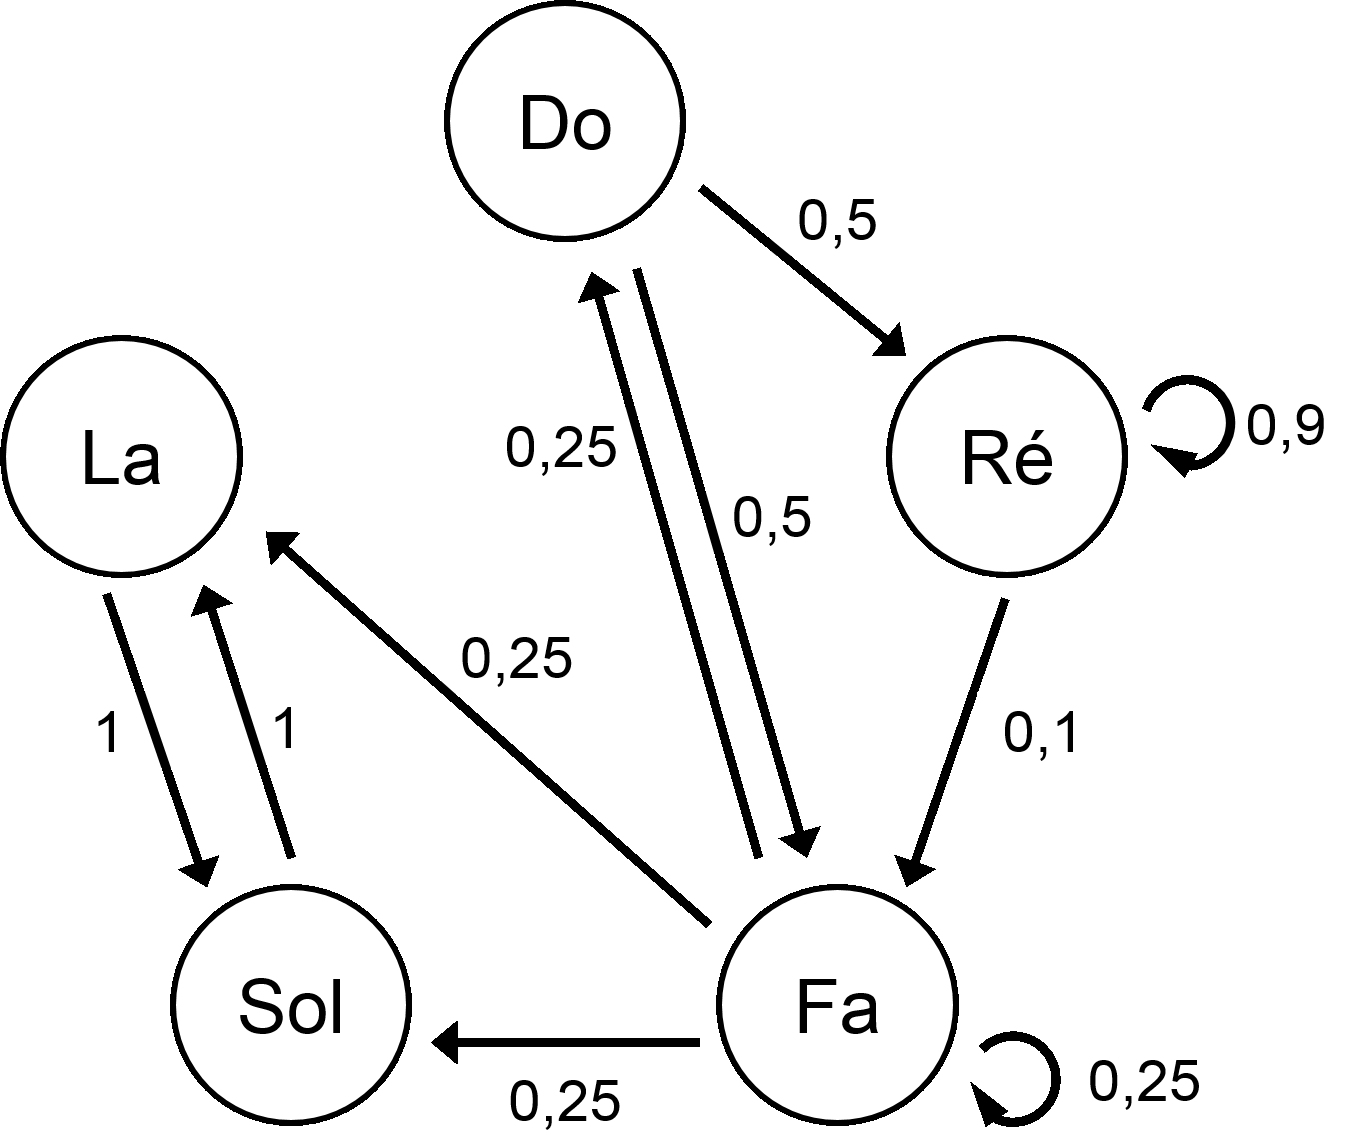
\includegraphics[width=7cm]{images/markov.png}~~~~~~~~~
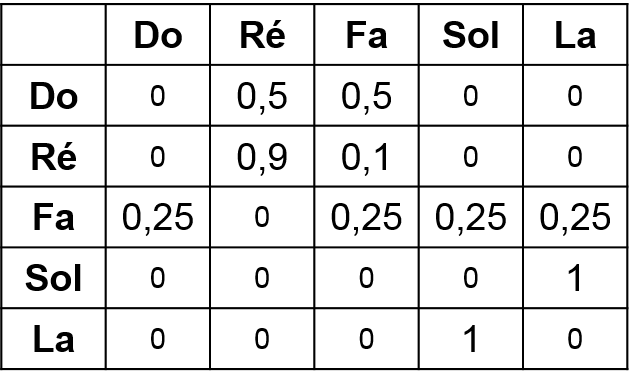
\includegraphics[width=6cm]{images/markov2.png}
\caption{\footnotesize Un exemple simplifié de chaîne de Markov telle qu'utilisée dans la musique stochastique, représentée sous forme de graphe et de tableau (les probabilités sont données entre 0 et 1, sur le graphe les transitions de probabilité nulle ne sont pas dessinées). Le matériau représenté consiste simplement en cinq notes d'une gamme pentatonique (do-ré-fa-sol-la). Il y a une chance sur deux pour que la note suivant un do soit un ré et une chance sur deux pour que ce soit un fa. La note suivant un ré est un autre ré avec probabilité 0.9, et un fa sinon. Après un fa, on peut avoir un autre fa, un do, un sol ou un la de manière équiprobable. La seule note pouvant suivre un sol est un la et réciproquement. La structure étant définie, on peut parcourir le graphe en utilisant des processus aléatoires, afin d'obtenir une suite de notes (par exemple, en partant d'un do : do-ré-ré-ré-ré-fa-do-fa-la-sol-la-sol-la-\dots). Ce sont des mécanismes similaires qui régissent la musique stochastique comme l'\emph{Illiac Suite} ou de nombreuses pièces de Xenakis.}
\label{markovexemple}
\end{center}
\end{figure}

Entre les jeux de dés musicaux et les opérations informatiques pseudo-aléatoires, il y a donc une régression qualitative dans l'utilisation du hasard. L'élément aléatoire est seulement simulé. Cela montre qu'Essl, comme la plupart des artistes, ne s'intéresse pas au hasard de manière ontologique, scientifique, ou métaphysique, mais qu'il exploite ses propriétés esthétiques dans ses compositions. Ce qui lui importe, c'est que les phénomènes sonores soient imprévisibles par l'auditeur, un hasard \emph{sensible} et non théorique. L'atout de l'ordinateur qui prend le pas est sa capacité à simuler le hasard très rapidement. À partir de l'exemple de la figure \ref{markovexemple}, on pourrait écrire des pièces en jetant des dés ; mais un ordinateur permettrait de le faire \emph{en temps réel}, ou encore de générer un grand nombre de séquences différentes. La présence dans la \emph{RTC-lib} d'un générateur de graines pour les fonctions aléatoires, \patch{RandomSeeder} (qui utilise la date et l'heure), atteste de la maîtrise de ce pseudo-hasard par Essl.

Le chercheur en informatique Philippe Codognet distingue deux utilisations du hasard à des fins esthétiques : le \emph{hasard interne}, ou recours au hasard pendant la composition de l'œuvre, et le \emph{hasard externe}, qui correspond aux éléments imprévisibles lors de son exécution \cicite{Assayag~et~al.,~2009,~p.~160} ; la meilleure illustration de hasard externe est à cet égard la pièce \emph{4'43''} de John Cage. Comme la composition en temps réel fait coïncider composition et interprétation, on pourrait attendre une rencontre de ces deux hasards. Mais le hasard externe n'apparaît qu'au travers de certaines possibilités interactives, généralement limitées, des pièces composées par Essl, ou dans les performances improvisées qu'il donne. C'est bien le hasard interne qui est prépondérant dans les fonctions de la \emph{RTC-lib} et des pièces comme la \emph{Lexikon-Sonate}.

\subsubsection{Le \guill{temps réel}}
\label{tempsreel}

La \guill{composition en temps réel} étant la notion la plus remarquable de l'œuvre d'Essl reposant sur le progrès technologique, il est intéressant d'étudier précisément les conditions historiques qui ont permis son apparition.

Il convient d'abord de préciser que, comme pour le hasard, il n'y a pas de \guill{temps réel} au sens d'une immédiateté dans l'interaction entre l'homme et la machine. Comme le rappelle le compositeur Philippe Manoury (1952-) : \guill{C'est en fait une illusion. Le temps réel n'existe jamais dans la réalité technologique parce qu'une machine met toujours un certain temps, même si celui-ci est extrêmement bref, pour effectuer ses calculs. \tpp~En musique, on parle de temps réel à partir du moment où le laps de temps entre le début du calcul et la livraison du résultat d'une opération informatique est suffisamment bref pour ne pas être perçu.} \cicite{Manoury~et~al.,~2012,~p.~41-42}. Ainsi, l'accent est à nouveau mis sur les perceptions de l'auditeur : ce qui est suffisamment bref pour sembler sans durée est appelé temps réel.

C'est en 1991 qu'Essl découvre la possibilité du temps réel, grâce à la Station d'informatique musicale de l'IRCAM. Cette \guill{station} est simplement un ordinateur central ou \emph{mainframe}, construit à partir d'ordinateurs NeXT et d'une carte son spécialisée. L'interaction en temps réel est une nouveauté considérable pour Essl par rapport à ce qu'il connaît sur son Atari ST personnel : \guill{En LOGO, il fallait de longues heures pour calculer une liste de données que je devais ensuite transformer en notation musicale pour pouvoir l'analyser--- une procédure qui prenait un temps considérable.} \cicite{Essl,~2010}. La figure \ref{tableaumips}\footnote{D'après \href{http://doornbusch.net/}{http://doornbusch.net/} et  \href{https://en.wikipedia.org/wiki/Instruœctions\_per\_second\#MIPS}{https://en.wikipedia.org/wiki/Instructions\_per\_second\#MIPS} (consultés le \today).} montre que la puissance de la Sim était effectivement bien supérieure à celle de l'Atari ST\footnote{Plus précisément, il s'agit des puissances des processeurs utilisés par ces ordinateurs, respectivement trois cartes avec deux Intel i860 de 1991 pour la Sim et le Motorola 68000 de 1982 pour l'Atari ST}. À cette époque, la génération de musique ou le traitement du son en temps réel étaient donc possibles sur des ordinateurs de type \emph{mainframe} mais pas sur les micro-ordinateurs : il s'agit du moment précis où le progrès technologique, incrémental, a permis leur réalisation, véritable progrès qualitatif.

\begin{figure}[!h]
\begin{center}
\begin{tabular}{|c|c|c|c|}
\hline
\textbf{Année} & \textbf{MIPS} & \textbf{Modèle} & \textbf{Type} \\
\hline
1954 & 0,000640 & IBM 704 & \emph{Mainframe} \\
\hline
1969 & 3,3 & IBM 360/85 & \emph{Mainframe} \\
\hline
1973 & 0,065500 & DEC PDP 11/45 & Micro \\
\hline
1977 & 0,230 & Apple II & Micro \\
\hline
\textbf{1985} & \textbf{2,188} & \textbf{Atari ST} & \textbf{Micro} \\
\hline
\textbf{1988} & \textbf{6$\times$50} & \textbf{Sim (IRCAM)} & \textbf{\emph{Mainframe}} \\
\hline
\textbf{1997} & \textbf{525} & \textbf{PowerBook G3} & \textbf{Micro} \\
\hline
2003 & 3100 & iMac G5 & Micro \\
\hline
2008 & 50000 & Apple Mac Pro & Micro \\
\hline
\end{tabular}
\caption{\footnotesize Tableau indiquant la puissance de quelques modèles d'ordinateurs, en millions d'instructions par seconde (MIPS) exécutables par le processeur. Il est précisé pour chacun s'il s'agit d'un \emph{mainframe} (ou \emph{ordinateur central}, machine centralisée de grande taille) ou d'un micro-ordinateur. Les modèles en gras correspondent à ceux utilisés par Essl dont il est question dans cette partie, les autres sont donnés à titre indicatif.}
\label{tableaumips}
\end{center}
\end{figure}

La différence entre les calculs de plusieurs heures d'Essl et le temps réel à l'IRCAM s'explique par deux facteurs supplémentaires. D'abord, Essl programmait avec le langage LOGO, et même avec une version interprétée de ce langage, nommée xLOGO, ce qui signifie que l'exécution des codes qu'il écrivait nécessitait une étape de \guill{traduction} vers un langage informatique plus simple. Ce langage offrait aussi une bien meilleure expressivité et des fonctionnalités plus étendues que, par exemple, le BASIC ; en contre-partie, des codes simples peuvent correspondre à un nombre important d'instructions machine élémentaires. La Sim, en revanche, utilisait le langage MAX, développé expressément pour elle et optimisé pour les tâches de musique algorithmique. En outre, même avec un langage plus performant et un ordinateur plus puissant, Essl aurait dû traduire les résultats de ses programmes en notation musicale. Le progrès matériel que représente la Sim réside dans l'association d'un ordinateur puissant avec une \emph{carte son}, c'est-à-dire un composant électronique dédié à l'interface entre l'unité de calcul et des périphériques audio comme des hauts-parleurs. Celle-ci peut prendre en charge une grande partie des calculs spécifiques au traitement du signal, grâce à quoi la conversion en son pouvait avoir lieu en \guill{temps réel}. De l'analyse de la \emph{RTC-lib} (section \ref{rtclib}), concluant que la plupart des fonctions étaient d'une complexité algorithmique faible, on déduit que l'aspect compositionnel de la \guill{composition en temps réel} n'exploitait même pas toutes les capacités de la Sim (et nécessite une puissance de calcul très en-deçà de celle des ordinateurs standards actuels). L'avancée déterminante pour permettre l'existence de cette notion se situait dans le traitement sonore \emph{via} la carte son, et non dans la puissance de calcul brute.

La figure \ref{tableaumips} montre que, du fait de l'augmentation rapide de la puissance des ordinateurs, l'Apple PowerBook G3 acheté par Essl en 1997 atteint et même dépasse les capacités de la Sim. Cette croissance est exponentielle : elle suit approximativement la loi empirique de Moore\footnote{Décrite dans \cicite{Moore,~2000}.}, qui affirme que le nombre de transistors sur un micro-processeur pouvant être fabriqué à un coût donné double tous les ans environ. C'est pourquoi de nombreux progrès ont lieu sur de très courtes échelles de temps. En ce qui concerne le \guill{temps réel} musical, il apparaît donc que les prototypes comme la Sim l'ont concrétisé dès qu'il a été technologiquement possible, de même qu'Essl dans un second temps, lorsqu'il a été accessible aux micro-ordinateurs.

\subsection{Un compositeur de l'ère numérique}
\label{internet}

Cette dernière partie traite d'un aspect peu abordé jusqu'ici du rôle de l'ordinateur dans le travail d'Essl, l'utilisation qu'il fait du réseau Internet. Les enjeux en sont moins technologiques que sociaux. La façon dont ce réseau mondial, qui est l'un des piliers de l'informatique au sens large et le principal moteur de la culture numérique, bouleverse l'activité du compositeur, mérite d'être étudiée. Internet ouvre de nouvelles perspective à la fois dans le rapport de l'artiste à l'œuvre, au public, et à ses homologues. Chez Essl, la redéfinition du rapport à l'œuvre passe avant tout par la question de l'auctorialité. Celle du rapport au public réside dans l'utilisation d'Internet comme medium de masse, moyen de diffusion efficace au service d'une volonté de démocratisation. Enfin, la communication joue un rôle important pour Essl en particulier parce qu'elle lui permet d'entrer en contact et de collaborer avec d'autres artistes.

De même que l'apparition des micro-ordinateurs et leur démocratisation, Essl a vécu leur mise en réseau qui a conduit à l'avènement d'Internet. L'origine de cette \guill{Toile} permettant de relier n'importe quels ordinateurs à l'échelle mondiale remonte aux années 1960. Arpanet, lancé en 1969, premier réseau à grande échelle reposant sur le principe de \emph{transfert par paquets}, est considéré comme son premier ancêtre. Les techniques d'échange de données entre ordinateurs évoluent rapidement et les réseaux se succèdent, en particulier Bitnet à partir de 1981, qu'Essl a connu pendant ses études \cicite{Ehrler,~1999}, et Internet depuis 1989. Ces réseaux permettent aux ordinateurs de servir d'interface pour l'échange de données à grande distance, symbolisé par le courrier électronique, inventé dès 1965.

La vitesse des communications et l'effacement des barrières géographiques qu'elle entraîne modifient radicalement les perspectives traditionnelles de circulation des informations. Ils font par exemple apparaître le problème de la surveillance et de la protection de la vie privée, ou celui du téléchargement illégal. Dans le cas d'Essl, comme de tout artiste, c'est justement la question du statut auctorial et de la distribution de ses œuvres ---~partitions, enregistrements, programmes --- qui est posée par le monde numérique. Sa position est intéressante. D'un côté, il cède une grande partie des privilèges traditionnels de l'auteur. Ainsi distribue-t-il la plupart de ses programmes\footnote{Seuls le \emph{REplay PLAYer} et \emph{fLOW} sont des \emph{sharewares}, c'est-à-dire qu'il en existe deux versions, l'une gratuite mais aux fonctionnalités limitées, l'autre complète mais payante.} sous licence libre, comme nous l'avons vu dans le cas de la \emph{Lexikon-Sonate} et dans celui de la \emph{RTC-lib}, qui sont pourtant respectivement son œuvre au plus grand succès et le socle logiciel de tout son travail algorithmique de composition. De même, Essl rend ses partitions disponibles et gratuites. Il met à disposition sur son site personnel de nombreux enregistrements de ses pièces, ainsi que sur sa chaîne YouTube où il rend publiques des performances, des entretiens et des cours (plus de 300 séquences vidéo à ce jour). Ce parti-pris s'explique grandement par le contexte historique. Comme cela a été mis en avant dans la partie \ref{parcoursalgo}, Essl fait partie de la génération qui a connu la généralisation des micro-ordinateurs et l'idéal de liberté à laquelle elle s'associe. À la même époque, dans le courant des années 1980, apparaît en outre le courant du logiciel libre\footnote{Plus précisément, ce sont les logiciels propriétaires qui apparaissent, le logiciel étant auparavant considéré comme un objet scientifique et circulait comme tel dans le milieu universitaire. Pour plus de détails sur l'histoire du logiciel libre, voir \cicite{Paloque-Berges~et~Masutti,~2013}.}, qui promeut le partage des ressources logicielles de tous vers tous et gratuitement, auquel Essl s'associe donc dans la distribution de ses travaux que nous venons d'évoquer. Chacun de ses programmes téléchargeables inclut ainsi une licence délimitant précisément les usages que peut en faire l'utilisateur, ce qui montre la préoccupation du compositeur sur cette question. Toutefois, il affirme dans le même temps son statut auctorial ainsi que sa propriété intellectuelle. Il ne s'oppose pas à ce que certaines exécutions de ses œuvres soient payantes, touchant des droits sur les concerts ou CD dans lesquels d'autres musiciens jouent ses compositions. Il lui arrive aussi, comme nous l'avons vu dans le cas de la \emph{Lexikon-Sonate}, de conserver une version améliorée de ses programmes exclusivement pour ses propres performances ; dans le cas de son instrument \maze, il n'existe même pas de version publique. Un événement dans le développement de la \emph{Lexikon-Sonate} est révélateur de l'intérêt porté par Essl à la question auctoriale : à l'origine, le programme possédait une sortie MIDI, mais Essl a découvert que \guill{des personnes l'ont utilisé pour générer des partitions. Comme si c'était un programme générateur de partitions. Et ils ont ainsi créé des morceaux qu'ils ont vendu comme leurs propres morceaux}\footnote{Entretien en annexe.}. Essl a donc désactivé la sortie MIDI de la version publique, consolidant ainsi sa position d'auteur.

L'une des spécificités du réseau Internet est qu'il \guill{met en jeu un type de liaison multimodale entre les utilisateurs sans précédent : la liaison de \emph{tous vers tous} [où] chaque internaute est à la fois récepteur et émetteur} \cicite{Couchot~et~Hillaire,~2003,~p.~63}. Remarquons avant tout qu'Essl n'exploite cependant pas tout ce potentiel : si, comme nous allons le voir, il tire profit de la liaison de \emph{un vers tous} pour la diffusion de son œuvre, il a peu recours à celle de \emph{tous vers un}, c'est-à-dire les possibilités d'interactivité. En ce sens, son utilisation du réseau mondial est la même que celle des media de masse (radio, télévision, cinéma), dont les propriétés sont simplement amplifiées par Internet. Cette limitation de l'interactivité est d'ailleurs une caractéristique générale de l'œuvre d'Essl. Contrairement à beaucoup d'autres compositeurs, il n'en fait pas un enjeu esthétique important ; ses programmes et installations permettent une interaction mais l'utilisateur a des possibilités restreintes plutôt qu'une liberté totale. Même son instrument \maze~n'est pas interactif au sens large : bien que certaines de ses fonctionnalités aient recours au hasard, celles-ci reposent toujours sur l'idée de \emph{Strukturgenerator}, et produisent donc une réponse imprévisible mais jamais imprévue aux stimuli qu'il reçoit.

On peut identifier dans la démarche d'Essl une véritable tentative de démocratisation de son travail, de le rendre accessible à la fois en termes intellectuels et logistiques. Dans sa démarche esthétique, ce pas vers le public passe par le refus d'une musique trop abstraite\footnote{\guill{Je ne fais pas de la musique abstraite qu'on ne peut comprendre que si l'on a une formation spéciale, ou des connaissances particulières, ou beaucoup d'expérience. Ce qui m'intéresse, c'est avant tout ce qu'il y a d'immédiat, d'extatique, qui se révèle à celui qui est prêt à s'abandonner.} \cicite{Essl~et~Kühnelt,~2006/2007} ; voir aussi \cicite{Essl~et~Günther,~1998}.}, l'utilisation de matériaux musicaux connus de tous\footnote{\guill{Je voulais délibérément utiliser un matériau très succinct, qui soit de plus facile à identifier. \tpp~Il existe ainsi certaines musiques très caractéristiques, comme aussi la \emph{Cinquième} de Beethoven ; \tpp~il suffit de les jouer et chacun sait immédiatement de quoi il s'agit.} \cicite{Essl~et~Huber,~2014}.}, ou d'une manière générale l'attachement au son et à l'effet qu'il produit à l'intérieur de la démarche algorithmique\footnote{\guill{Je crois que l'algorithme ne doit jamais devenir un fétiche se suffisant à lui même, à la logique duquel il faudrait faire appel pour dire : cette structure est si belle, si mathématique à tous points de vue, si cohérente. Cela doit toujours passer à l'épreuve de la réalité et de notre expérience d'auditeurs.} \cicite{Förster,~2011}.}. Sur le plan pratique, il s'incarne dans la recherche de lieux de concerts non-traditionnels comme les musées, en particulier le Essl Museum, et naturellement dans l'utilisation d'Internet pour diffuser son œuvre. Les aspects de \guill{liberté} déjà évoqués dans la diffusion d'enregistrements et de programmes y participe. De plus, Essl multiplie les lieux virtuels de sa présence sur Internet : les réseaux sociaux Twitter et Facebook, les plate-formes de distribution audio et vidéo SoundCloud et YouTube, ainsi que sa page personnelle\footnote{\href{http://www.essl.at}{http://www.essl.at} (consultée le \today) sur laquelle on trouvera quelques remarques dans \cicite{Ehrler,~1999}.}. Celle-ci fait office à la fois de vitrine \cicite{Essl~et~Pagano,~2009} et de musée --- \guill{L'Internet apparaît \tpp~comme le lieu de [la] mémoire à venir, comme musée virtuel global.} \cicite{Couchot~et~Hillaire,~2003,~p.~231}. Essl y propose, outre des liens pour télécharger ses programmes ou consulter ses séquences vidéos et enregistrements, sa propre actualité (compositions, concerts), de nombreux éléments biographiques, une liste exhaustive de ses écrits, et un recensement des publications à son propos. Cela représente un travail considérable qui lui permet de faire sa propre muséification. On peut cependant se demander si cette démarche n'est pas une condition nécessaire de visibilité donc d'existence dans un monde globalisé, saturé de communication et soumis à une très forte concurrence, y compris dans le domaine artistique. De même, on peut s'interroger sur la portée de la démocratisation qu'elle vise, car comme le soulignent Hillaire et Couchot : \guill{L'ambitieuse volonté d'une communication universelle est contrecarrée par la réalité. Le public attendu, innombrable, multi et transculturel, reste encore un public de spécialistes très liés au monde de l'art et très identifiables socialement. Les \guilldeux{communautés virtuelles} sont en fait des microcosmes assez fermés, avec déjà leurs traditions et leurs orthodoxies.} \cicite{Couchot~et~Hillaire,~2003,~p.79}.

Enfin, la dimension communicationnelle d'Internet joue, d'après Essl\footnote{\guill{D'après mon expérience personnelle, je pense que [l'aspect spécifique d'Internet] le plus important est la communication.} \cicite{Essl~et~Föllmer,~2004}.}, un rôle crucial dans son parcours. Il s'agit en l'occurrence bien d'une liaison \emph{tous vers tous}, qui implique non pas le public mais d'autres artistes. Comme cela a été expliqué dans la partie \ref{liberte}, Essl a donné une orientation nouvelle à sa carrière de compositeur après sa présentation au Festival de Salzbourg de 1997, en ouvrant sa pratique, et en particulier en collaborant avec d'autre musiciens\footnote{\guill{À travers le contact avec des pairs partageant mes goûts, qui avait d'abord lieu principalement grâce à des \emph{mailing lists}, j'ai mûri de nouvelles idées. \tpp~Le caractère non-hiérarchique d'Internet, avec sa structure rhizomatique, possède de multiples points communs avec ma propre vision d'une musique comme un réseau de communication dont on peut faire l'expérience sensible} \cicite{Essl~et~Föllmer,~2004}.}. Dans cette optique, sa page personnelle peut ainsi être comprise non seulement comme un moyen de visibilité envers le public mais aussi, avec la facilité de contact qu'elle propose, une invitation tacite à la collaboration pour les artistes qui la consulteraient. L'activité soutenue d'enseignement menée par Essl, à l'Académie de musique et des arts du spectacle de Vienne, mais aussi en tant que professeur invité dans des universités du monde entier, et dans les programmes \guill{pédagogiques} \cicite{Klein,~2013} qu'il propose au Essl Museum, souligne aussi l'importance que revêt pour lui la communication. On peut donc dire que l'avènement du réseau Internet a fait d'Essl, comme de tant d'autres, un citoyen global, et qu'il a immédiatement tiré profit des possibilités ouvertes par ce nouveau medium et en a fait un enjeu central de sa pratique artistique, la rendant plus collaborative.

Ces quelques remarques ébauchent la façon dont Essl utilise au compte de sa pratique artistique la révolution Internet. Le réseau est avant tout utilisé comme un medium, c'est-à-dire un outil de diffusion d'information et de communication. Il est mis au service de l'œuvre, en particulier de sa visibilité, mais sans sacrifier l'image de l'auteur. Essl ne s'efface pas derrière ses créations, et affirme au contraire son individualité.

\subsection{Conclusion : Essl et l'ordinateur}

Dans les différentes analyses qui précèdent, le rapport qui se dessine entre Essl et l'ordinateur, et plus généralement le monde numérique, est celui d'un artisan avec son outil. C'est ainsi qu'on a parlé de \guill{boîte à \emph{outils}} à propos de la \emph{RTC-lib} et de la façon dont elle est utilisée dans la \emph{Lexikon-Sonate} ; et on a vu qu'il utilise le réseau Internet avant tout comme un \emph{outil} de diffusion. Comme l'écrit le musicologue Bernhard Günther : \guill{Essl utilise les possibilités techniques actuelles comme un moyen de créer des structures musicales} \cicite{Günther,~1995} : un moyen, et non une fin. L'étude de ses programmes montre bien que c'est l'aspect sensible\footnote{Se ramener exclusivement aux sens, comme l'affirme Essl, est exagéré : il serait plus juste de parler de la tradition musicale historique. Si l'écoute apparaît primordiale, les procédés issus du sérialisme qui en sont déconnectés ont aussi une place conséquente dans l'œuvre d'Essl. On a cependant conservé ce terme de \guill{sensible} pour marquer l'opposition avec l'expérimentation abstraite des possibilités spécifiques de l'ordinateur.} qui a le dernier mot dans le processus de création, qu'Essl cherche à tirer parti de cet outil informatique pour donner vie à des idées musicales, et non à programmer des structures complexes pour leur donner ensuite un sens musical. Ce rapport à l'ordinateur comme outil transparaît aussi dans le modèle qu'utilise Essl : un PowerBook, à la fois moins performant que les appareils standards actuels, et antinomique de sa philosophie du libre. Il le reconnaît lui-même\footnote{Voir entretien en annexe.}, justifiant ce choix par le fait qu'il est \guill{plus productif} avec cet ordinateur auquel il est habitué. En outre, les analyses de la \emph{RTC-lib} et de la \emph{Lexikon-Sonate} ont montré à la fois qu'Essl possédait une véritable maîtrise de cet outil bien qu'il ne soit pas spécifique au domaine musical, et qu'il subissait aussi ses contraintes intrinsèques.

Il en résulte un rapport de force entre la technologie et le compositeur. Essl affirme sa singularité d'artiste et refuse que la technologie prenne le pas sur l'art. La limitation de l'interactivité dans ses créations ou encore le rejet des techniques d'intelligence artificielle pour la composition\footnote{Voir entretien en annexe.} montrent qu'il est musicien avant d'être programmeur. Bien que les algorithmes bénéficient d'un statut de premier plan dans son œuvre, ils ne le sont jamais au détriment des phénomènes sonores.

Il y a cependant une dimension exploratoire dans ce rapport à l'outil informatique, et donc créatif. Essl n'est pas un simple utilisateur, comme ce serait le cas s'il n'exploitait que des logiciels centrés sur un séquenceur, qui définissent nécessairement une orientation esthétique forte\footnote{Comme \emph{ProTools}, \emph{Cubase}, \emph{Ableton Live}\dots}, mais s'est approprié des langages de programmation afin de pouvoir développer plus librement ses propres idées. Il affirme même la programmation comme un impératif du compositeur informatique : \guill{Nous devons programmer l'ordinateur nous-même, autrement dit nous devons formuler nos idées compositionnelles propres, personnelles, individuelles, et nos propres interrogations sous la forme de programmes informatiques} \cicite{Förster,~2011}. On a ainsi exhibé à la fois l'exploitation de l'ordinateur pour mettre en œuvre des idées musicales préexistantes, mais aussi l'élaboration de nouvelles formes et notions, en particulier la composition en temps réelle, qu'Essl a développée dès le moment où elle a été technologiquement possible.

Le travail d'Essl a ainsi réalisé un progrès manifeste. C'est un progrès esthétique\footnote{La notion de \emph{progrès}, en science et dans le domaine des arts, est employée telle qu'elle est discutée dans \cicite{Kuhn,~1972}.}, et non scientifique ou technique --- Essl n'a pas par exemple conçu les machines qu'il utilise ---, mais fondé sur l'exploitation des possibilités des progrès techniques --- dans le cas de la composition en temps réel, l'augmentation de puissance des ordinateurs et dans une moindre mesure le développement du langage MAX. En résumé, il s'agit d'une approche \emph{opportuniste} de la technologie. Essl ne provoque pas les innovations technologiques mais apprend à maîtriser les possibilités disponibles, pour en tirer profit dans son travail artistique.

%\zitat{My formal thinking takes place in a bipolar field of tension, namely that between work and process. (…) For me, the most captivating aspect of composing is the reconciliation of these opposites, though each time in a different way.}
%{Composing in a Changing Society - How does a composition come into existence ?}


\section{Conclusion}

Fasciné comme toute une génération par la démocratisation des micro-ordinateurs et leur mise en réseau à l'échelle mondiale, Karlheinz Essl a pleinement incorporé cette nouvelle technologie dans son art. Musique électronique et synthèse sonore, composition algorithmique puis composition en temps réel, installations, méta-instruments, œuvres collaboratives : il n'a cessé d'explorer les nouvelles formes d'expression musicale permises par l'informatique. Son intérêt permanent pour la musique numérique d'avant-garde lui a permis de développer en pionnier, dès le moment de sa possibilité technique, la notion de composition en temps réel, synthèse des méthodes de composition algorithmique et du traitement du signal sonore en \guill{temps réel}, qui représente un véritable progrès dans l'exploitation de l'informatique par la musique savante.

L'analyse de ses programmes montre cependant qu'Essl s'inscrit dans la continuité de sa discipline, réfléchissant en termes musicaux et de créativité sans être attiré par les possibilités techniques qui lui semblent sans lien avec la tradition artistique ou les perceptions de l'auditeur. L'ordinateur est pour lui un exécutant rapide d'algorithmes de composition, un générateur de hasard, un interprète infatigable, un vecteur de diffusion et un moyen de communication, en somme un moyen pour parvenir à ses fins artistiques, un outil, central dans sa pratique quoique inféodé à l'artiste.

Dans l'histoire de la musique, Essl apparaît comme l'héritier esthétique de Gottfried Michael Koenig et de l'Institut de Sonologie, place forte du développement de la musique algorithmique. Leur tradition est celle d'une musique générative, où le compositeur élabore l'architecture d'ensemble de ses créations, et où les finitions sont confiées au hasard et à l'ordinateur. L'apport d'Essl a été d'explorer les développements de cette démarche à la lumière des progrès matériels et logiciels de l'informatique. Il s'agit naturellement d'une façon parmi d'autres de donner un sens à la technologie dans le champ musical savant. Elle s'oppose notamment aux recherches esthétiques de Xenakis et de son école, à l'origine par exemple de l'environnement de programmation \emph{IanniX}, chez qui la musique algorithmique a recours à des procédés plus abstraits et plus complexes, qui contrôlent la structure générale des morceaux, ont recours à des outils mathématiques extra-musicaux, et travaillent le son avec des méthodes aléatoires continues plutôt que discrètes.

Le rapport qu'entretient Essl à l'ordinateur est emblématique de sa génération, qu'il s'agisse du rôle de l'informatique dans la musique ou dans la société en général. Ses prédécesseurs, comme Koenig ou Stockhausen, ont été les témoins de la naissance de l'informatique moderne. Maîtrisant déjà la musique électronique, ils ont intégré en pionniers cette nouvelle science, objet de curiosité et de fantasmes, à la musique savante. Ses successeurs \footnote{Nommons à titre d'exemple Thor Magnusson (1972-), développeur de l'environnement de \emph{live coding} \emph{ixi lang}, ou Nick Collins (1975-) et Alex McLean (1975-), inventeurs des \emph{algoraves}, événements dansants autour de musique \emph{live coded}.}, qui ont grandi dans un monde numérique, déjà informatisé, font de l'ordinateur et de tout ce qui y a trait un objet commun des représentations. C'est ainsi que la pratique du \emph{live coding} propose au public de voir le code informatique au cours de son élaboration, supposant une familiarité du public suffisante pour apprécier les compétences techniques aussi bien qu'artistiques du performeur. Chez Essl, l'ordinateur reste privé et la programmation, hors du temps ; mais l'informatique n'est plus une composante exceptionnelle de l'œuvre, c'est un outil maîtrisé et omniprésent, un élément essentiel, indispensable sans être banal, de la table de travail du compositeur.

\newpage
{\footnotesize\begin{abstract}\footnotesize\renewcommand{\baselinestretch}{1.2}
L'informatique est omniprésente dans l'œuvre du compositeur contemporain autrichien Karlheinz Essl (1960-), qui produit aussi bien des partitions que des programmes, des installations interactives ou des performances avec ordinateur. L'objet de ce document est d'étudier son cas, dans une approche historique, comme un exemple de l'assimilation de l'informatique par l'art contemporain.

Une première partie fait l'étude historique du parcours d'Essl. Celui-ci est décrit en quatre étapes. D'abord, les années d'études du compositeur (jusqu'en 1984), au cours desquelles se forment ses principales influences qui le prédisposeront à s'intéresser à l'informatique. Ensuite (1984-1991), Essl fait ses premiers pas dans ce domaine suite à l'acquisition d'un premier ordinateur personnel, s'initiant à la programmation et intégrant des aspects algorithmiques à ses compositions. Plus tard (1991-1997), il développe ses travaux algorithmiques en leur associant une exécution en \guill{temps réel} : il crée des morceaux générés par ordinateur et joués au même moment, ce qu'il nomme la \emph{composition en temps réel}. Cette démarche qui était auparavant technologiquement impossible est permise par un ordinateur prototypique dédié à la musique construit à l'IRCAM, qu'Essl découvre lors d'un stage en 1991. Un dernier tournant a lieu en 1997, lorsque Essl décide de devenir \emph{performeur} en plus de compositeur, concevant notamment son propre instrument virtuel qu'il utilise dans des performances improvisées.

La seconde partie étudie l'utilisation de l'informatique par Essl et le rôle qu'elle joue dans son œuvre à partir de l'étude de ses programmes. Ces programmes, en particulier la bibliothèque \emph{RTC-lib} qui fournit des fonctions à la plupart de ses morceaux informatisés, et sa pièce emblématique, la \emph{Lexikon-Sonate}, sont considérés en tant que sources historiques. Leur analyse dégage les différents aspects du rapport d'Essl à l'ordinateur, qu'il utilise comme un outil au service d'idées musicales, privilégiant la programmation de fonctions simples et sensiblement intelligibles. La discussion des notions de \guill{hasard} et de \guill{temps réels} en informatique révèle une approche opportuniste de la technologie : Essl exploite les possibilités permises par le progrès technique sans les provoquer. Enfin il est montré que ces caractéristiques trouvent un écho dans l'utilisation que le compositeur fait du réseau Internet.

\end{abstract}
\bigskip
\textbf{Mots-clefs :}
\begin{itemize}
\item Karlheinz Essl
\item informatique musicale
\item musique algorithmique
\item composition en temps réel
\item code source
\item histoire de l'informatique
\end{itemize}}

\newpage
\nocite{*}
\section{Bibliographie}

\defbibheading{interviews}{\subsubsection*{Interviews}}
\defbibheading{articles}{\subsubsection*{Articles théoriques}}
\defbibheading{oeuvres}{\subsubsection*{Œuvres}}
\defbibheading{secondaires}{\subsection*{Sources secondaires}}
\setlength{\bibitemsep}{0pt}
%\setlength{\bibnamesep}{0pt}
%\setlength{\bibinitsep}{0pt}
\renewcommand{\bibfont}{\small}


\subsection*{Sources primaires}
\printbibliography[heading=interviews,subtype=interview]
\printbibliography[heading=articles,subtype=article]
\printbibliography[heading=oeuvres,subtype=oeuvre]


\printbibliography[heading=secondaires,subtype=secondaire]

\end{document}
